\part{Experimental Apparatus}
\label{Part2}
The \autoref{Part2} of this thesis gives a brief description of the experimental apparatus that provides the physical environment and data collection for analyses described in \autoref{Part3} and \autoref{Part4}. Questions raised in \autoref{sec:Flavor} require the refinement of our knowledge of nature at its smallest scale. The \ac{LHC} is best prepared to help us achieve this goal as it is the most powerful particle physics accelerator in the world, colliding protons at a center-of-mass energy of 13.6 TeV in 2023. The \ac{CMS} detector is one of several detectors that is capable of recording data under the harsh physical environment created by the \ac{LHC}. The \autoref{Part2} is organized as follows. \autoref{chap:LHC} discusses the \ac{LHC} and its surrounding \ac{CERN} accelerator complex. An overview of the \ac{CMS} detector is given in \autoref{chap:CMS}. Details on event reconstruction in \ac{CMS} are given in \autoref{chap:Event}. I personally contributed to the \ac{CMS} operations (taking responsibilities in roles such as the shifter leader, technical shifter, and Tracker \ac{DOC} expert) and Phase-2 Upgrade, which are discussed in \autoref{chap:Ops} and \autoref{chap:Upgrade}, respectively. Materials presented in \autoref{chap:LHC}-\autoref{chap:Event} are borrowed from various publications and public documents, to which I made no direct contributions. Except where noted, materials (i.e. figures and tables) presented in \autoref{chap:Upgrade} are prepared by myself.
\chapter{The Large Hadron Collider}
\label{chap:LHC}

The \ac{LHC}~\cite{Evans:2008zzb} is a circular particle physics accelerator located near Geneva, Switzerland. It collides protons at four interaction points, which correspond to the four major experiments hosted by the \ac{LHC}: the \ac{ALICE}~\cite{ALICE:2008ngc}, \ac{ATLAS}~\cite{ATLAS:2008xda}, \ac{CMS}~\cite{CMS:2008xjf}, and \ac{LHCb}~\cite{LHCb:2008vvz} experiments. Accelerating proton beams to TeV-level requires a chain of acceleration stages before they are energetic enough for the final injection into the \ac{LHC} ring. These stages of acceleration and the whole \ac{CERN} accelerator complex are discussed in \autoref{sec:CERN}. The number of collision events delivered by the \ac{LHC} is measured in units called ``luminosity''. The definition of luminosity is discussed in \autoref{sec:Lumi}. The long term schedule for the \ac{LHC} is discussed in \autoref{sec:Plan}.

\section{The CERN Accelerator Complex}
\label{sec:CERN}

Installed in a 27 km circular tunnel previously used for the \ac{LEP} collider~\cite{203828}, the \ac{LHC} is the largest and most powerful particle accelerator ever existed. The primary objective of the \ac{LHC} is to deliver high intensity and high energy proton collisions, allowing physicists to study the laws of nature at the most fundamental scale. This objective is achieved through a complex system of accelerators, which rapidly accelerates protons to the target energy in a multistage process, maintains the proton energy, focuses, and collides them precisely at the designated locations. The full system is illustrated in Figure~\ref{fig:LHC}.

\begin{figure}[tbh!]
 \begin{center}
 \begin{tabular}{c}
 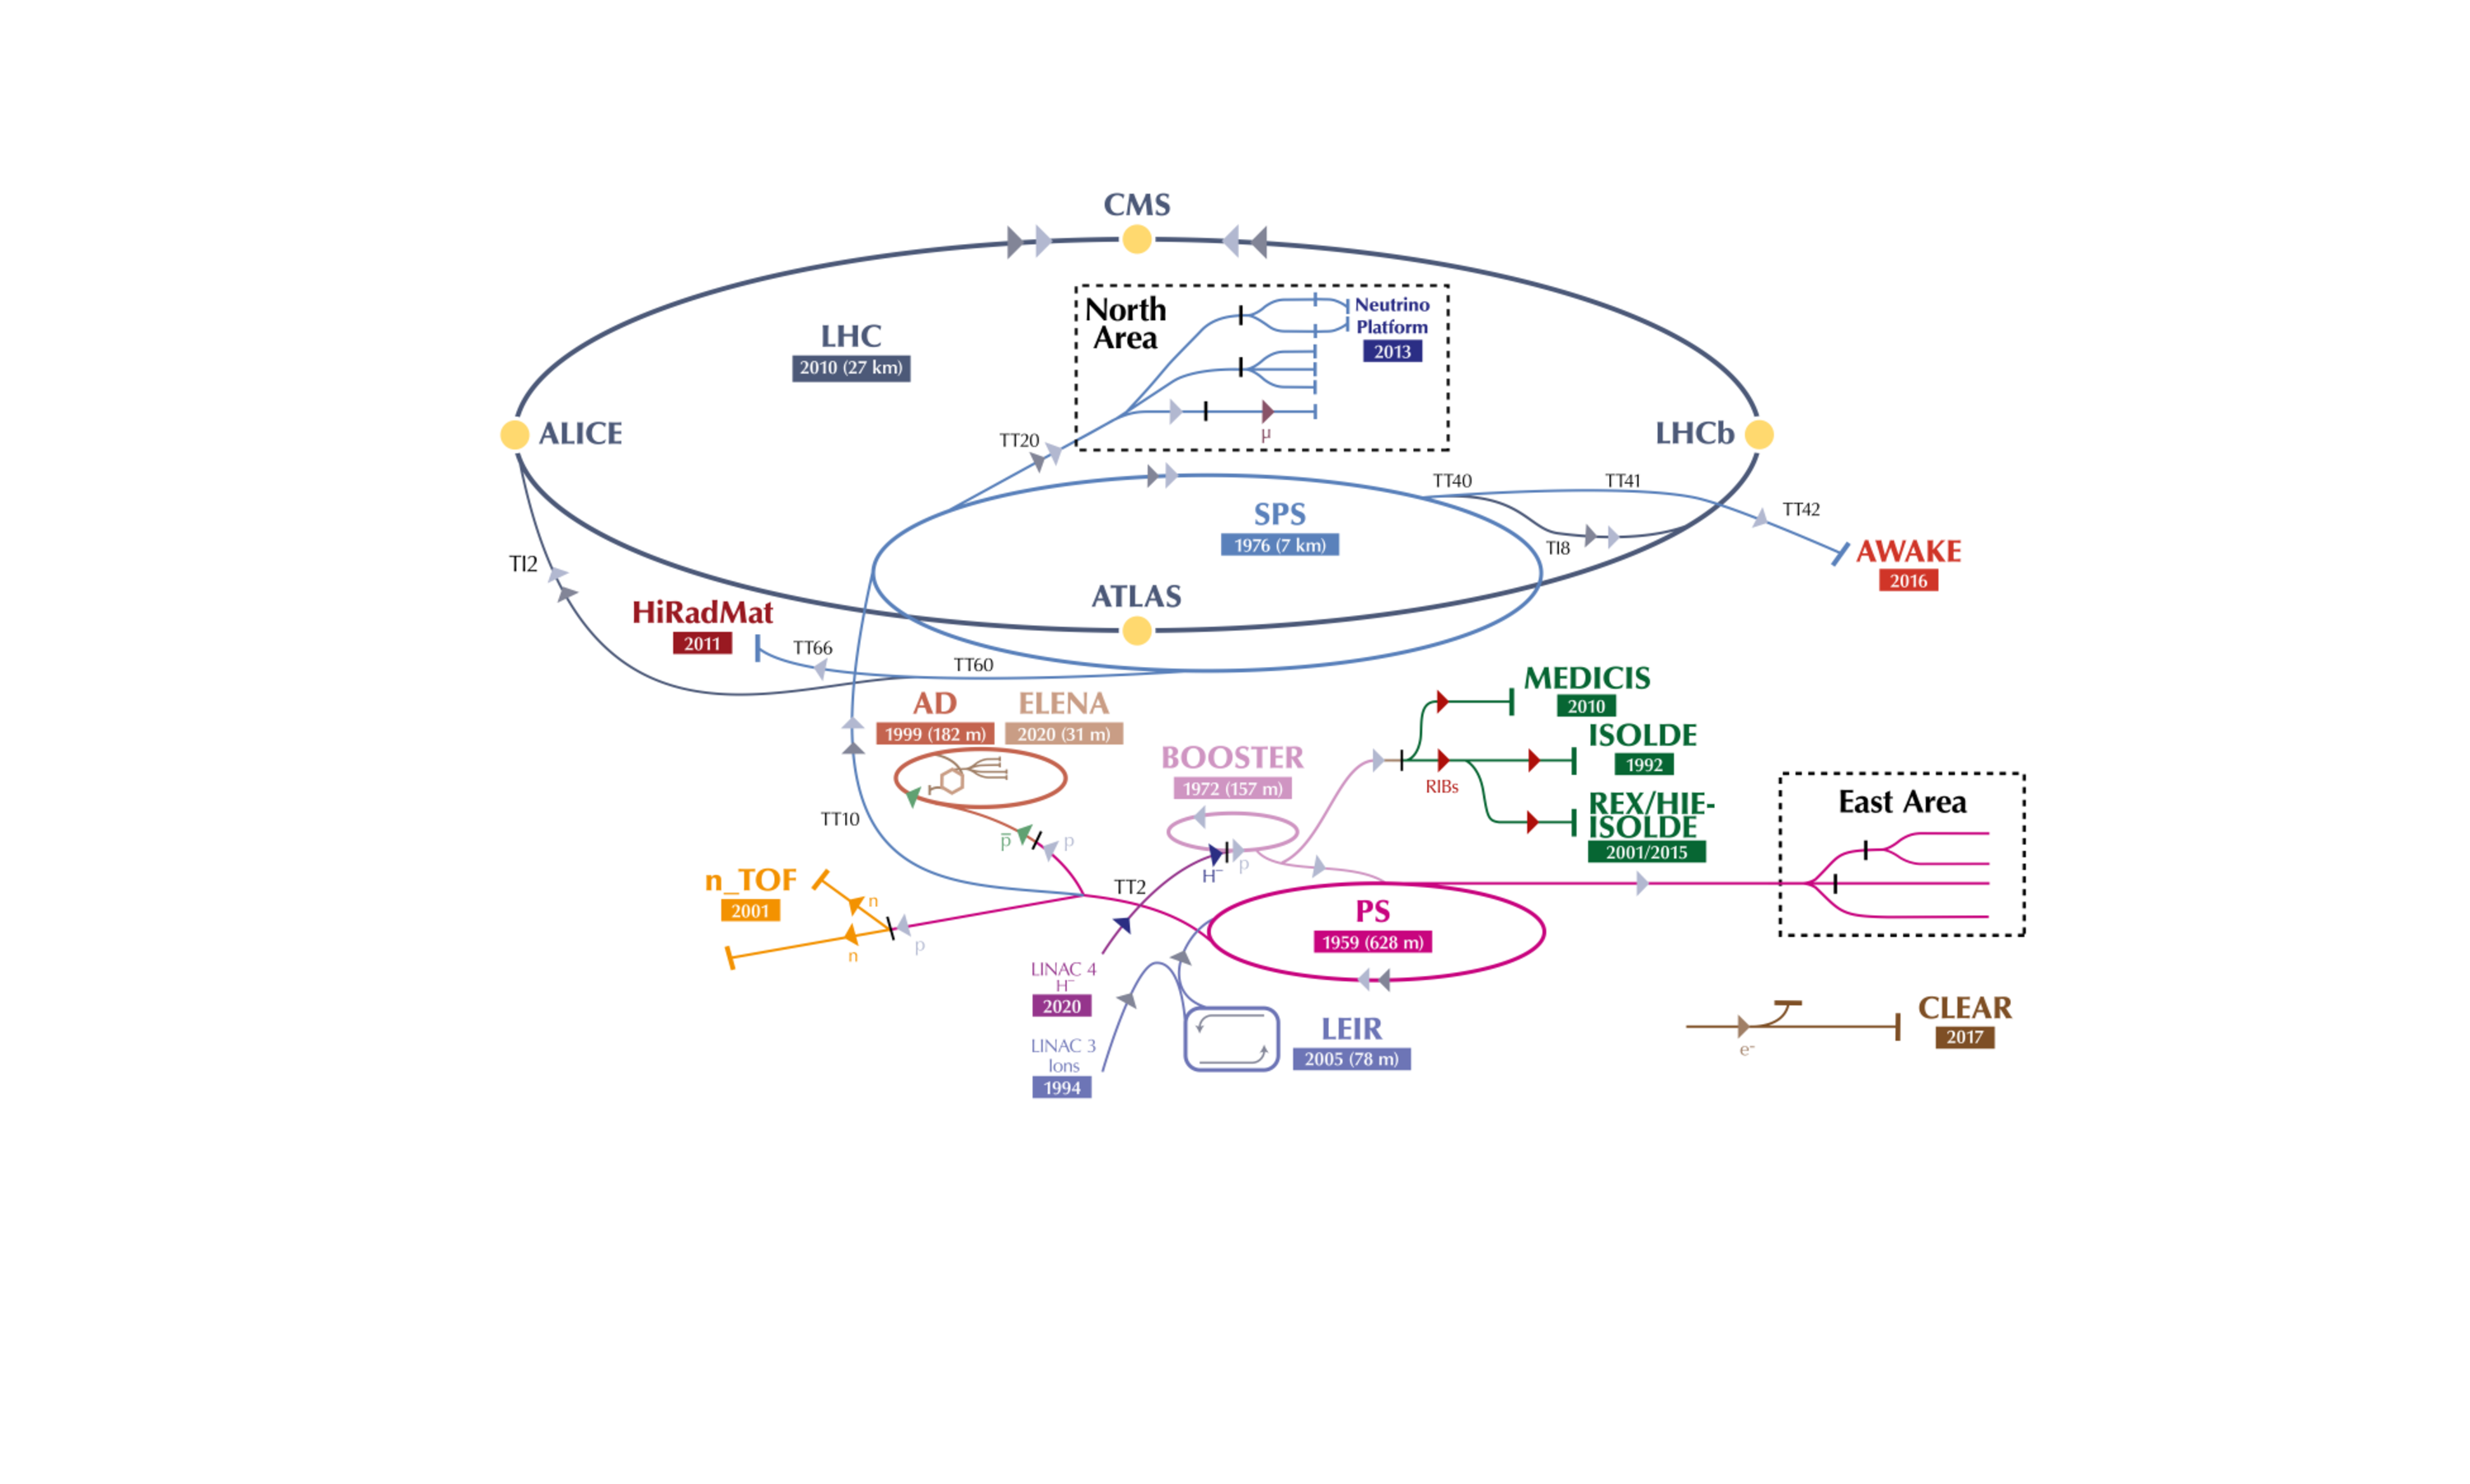
\includegraphics[width=\textwidth]{figures/Part2/LHC/CERN}
 \end{tabular}
 \caption{Layout of the \ac{CERN} accelerator complex, adapted from~\cite{CERN:2022}.}
 \label{fig:LHC}
 \end{center}
\end{figure}

Until 2018, an older linear accelerator (LINAC 2) was used to initially accelerate protons to 50 MeV. After 2018, negative hydrogen ions (H$^{-}$) are accelerated by the Linear accelerator 4 (LINAC 4)~\cite{Vretenar:2020quc} to 160 MeV using cylindrical conductors charged by radiofrequency cavities. Quadrupole magnets are placed along the accelerator to keep the beam focused.  The hydrogen ions are then stripped of their two electrons during injection into the Proton Synchrotron Booster (BOOSTER)~\cite{Reich:1969fw}, which is a circular accelerator that boosts protons to 2 GeV. Protons are then injected into the Proton Synchrotron (PS), which accelerates them to 25 GeV before injecting them into the second largest machine in the accelerator complex called the \ac{SPS}. The \ac{SPS} is a 7 km circular accelerator that uses room-temperature dipole magnets to bend the protons. Protons are accelerated by the \ac{SPS} to an energy of 450 GeV before entering the final accelerator ring -- the \ac{LHC}. The \ac{LHC} uses super-conducting dipole magnets up to 8.4 T to bend protons and ultimately accelerate them to 6.8 TeV during Run-3. Quadrupole magnets are placed at four collision points to focus the proton beams, which eventually collide at the \ac{IP} of each detector. 

\section{Luminosity}
\label{sec:Lumi}

The total number of events of a given process is given by 

\begin{equation}
N=\int\mathcal{L}\sigma dt,
\end{equation}

where $\sigma$ is the cross-section of the process and $\mathcal{L}$ is known as the instantaneous luminosity that can be written in a simplified form

\begin{equation}
\mathcal{L}=\frac{N^2f}{A},
\end{equation}

where $N$ is the total number of protons in each beam, $f$ is the frequency of the beam crossing, and $A$ is the cross-sectional area of the beam crossing.

The \ac{LHC} is designed to deliver an instantaneous luminosity $\mathcal{L}=10^{34}\textsf{cm}^{-2}~\textsf{s}^{-1}$ which corresponds to an event rate of 1 billion collisions per second, assuming the inelastic cross-section $\sigma^{\textsf{pp}}_{\textsf{in}}~=$ 100 mb. The delivered integrated luminosity by year of data taking is shown in Figure~\ref{fig:twikilumi}.

The peak instantaneous luminosity reached $2\times10^{34}~\textsf{cm}^{-2}\textsf{s}^{-1}$ in 2018, which is factor of two larger than the design value of the \ac{LHC}. High instantaneous luminosity means more collision events are delivered by the \ac{LHC}, but it also brings a side effect -- multiple interactions per crossing, also known as \ac{PU} . The average number of \ac{PU} increased from 27 in 2016 to 52 in 2023, creating challenges for data-taking and event reconstruction. The \ac{PU} profile for each year of data taking is shown in \ref{fig:twikilumi}.

\begin{figure}[tbh!]
 \begin{center}
 \begin{tabular}{cc}
 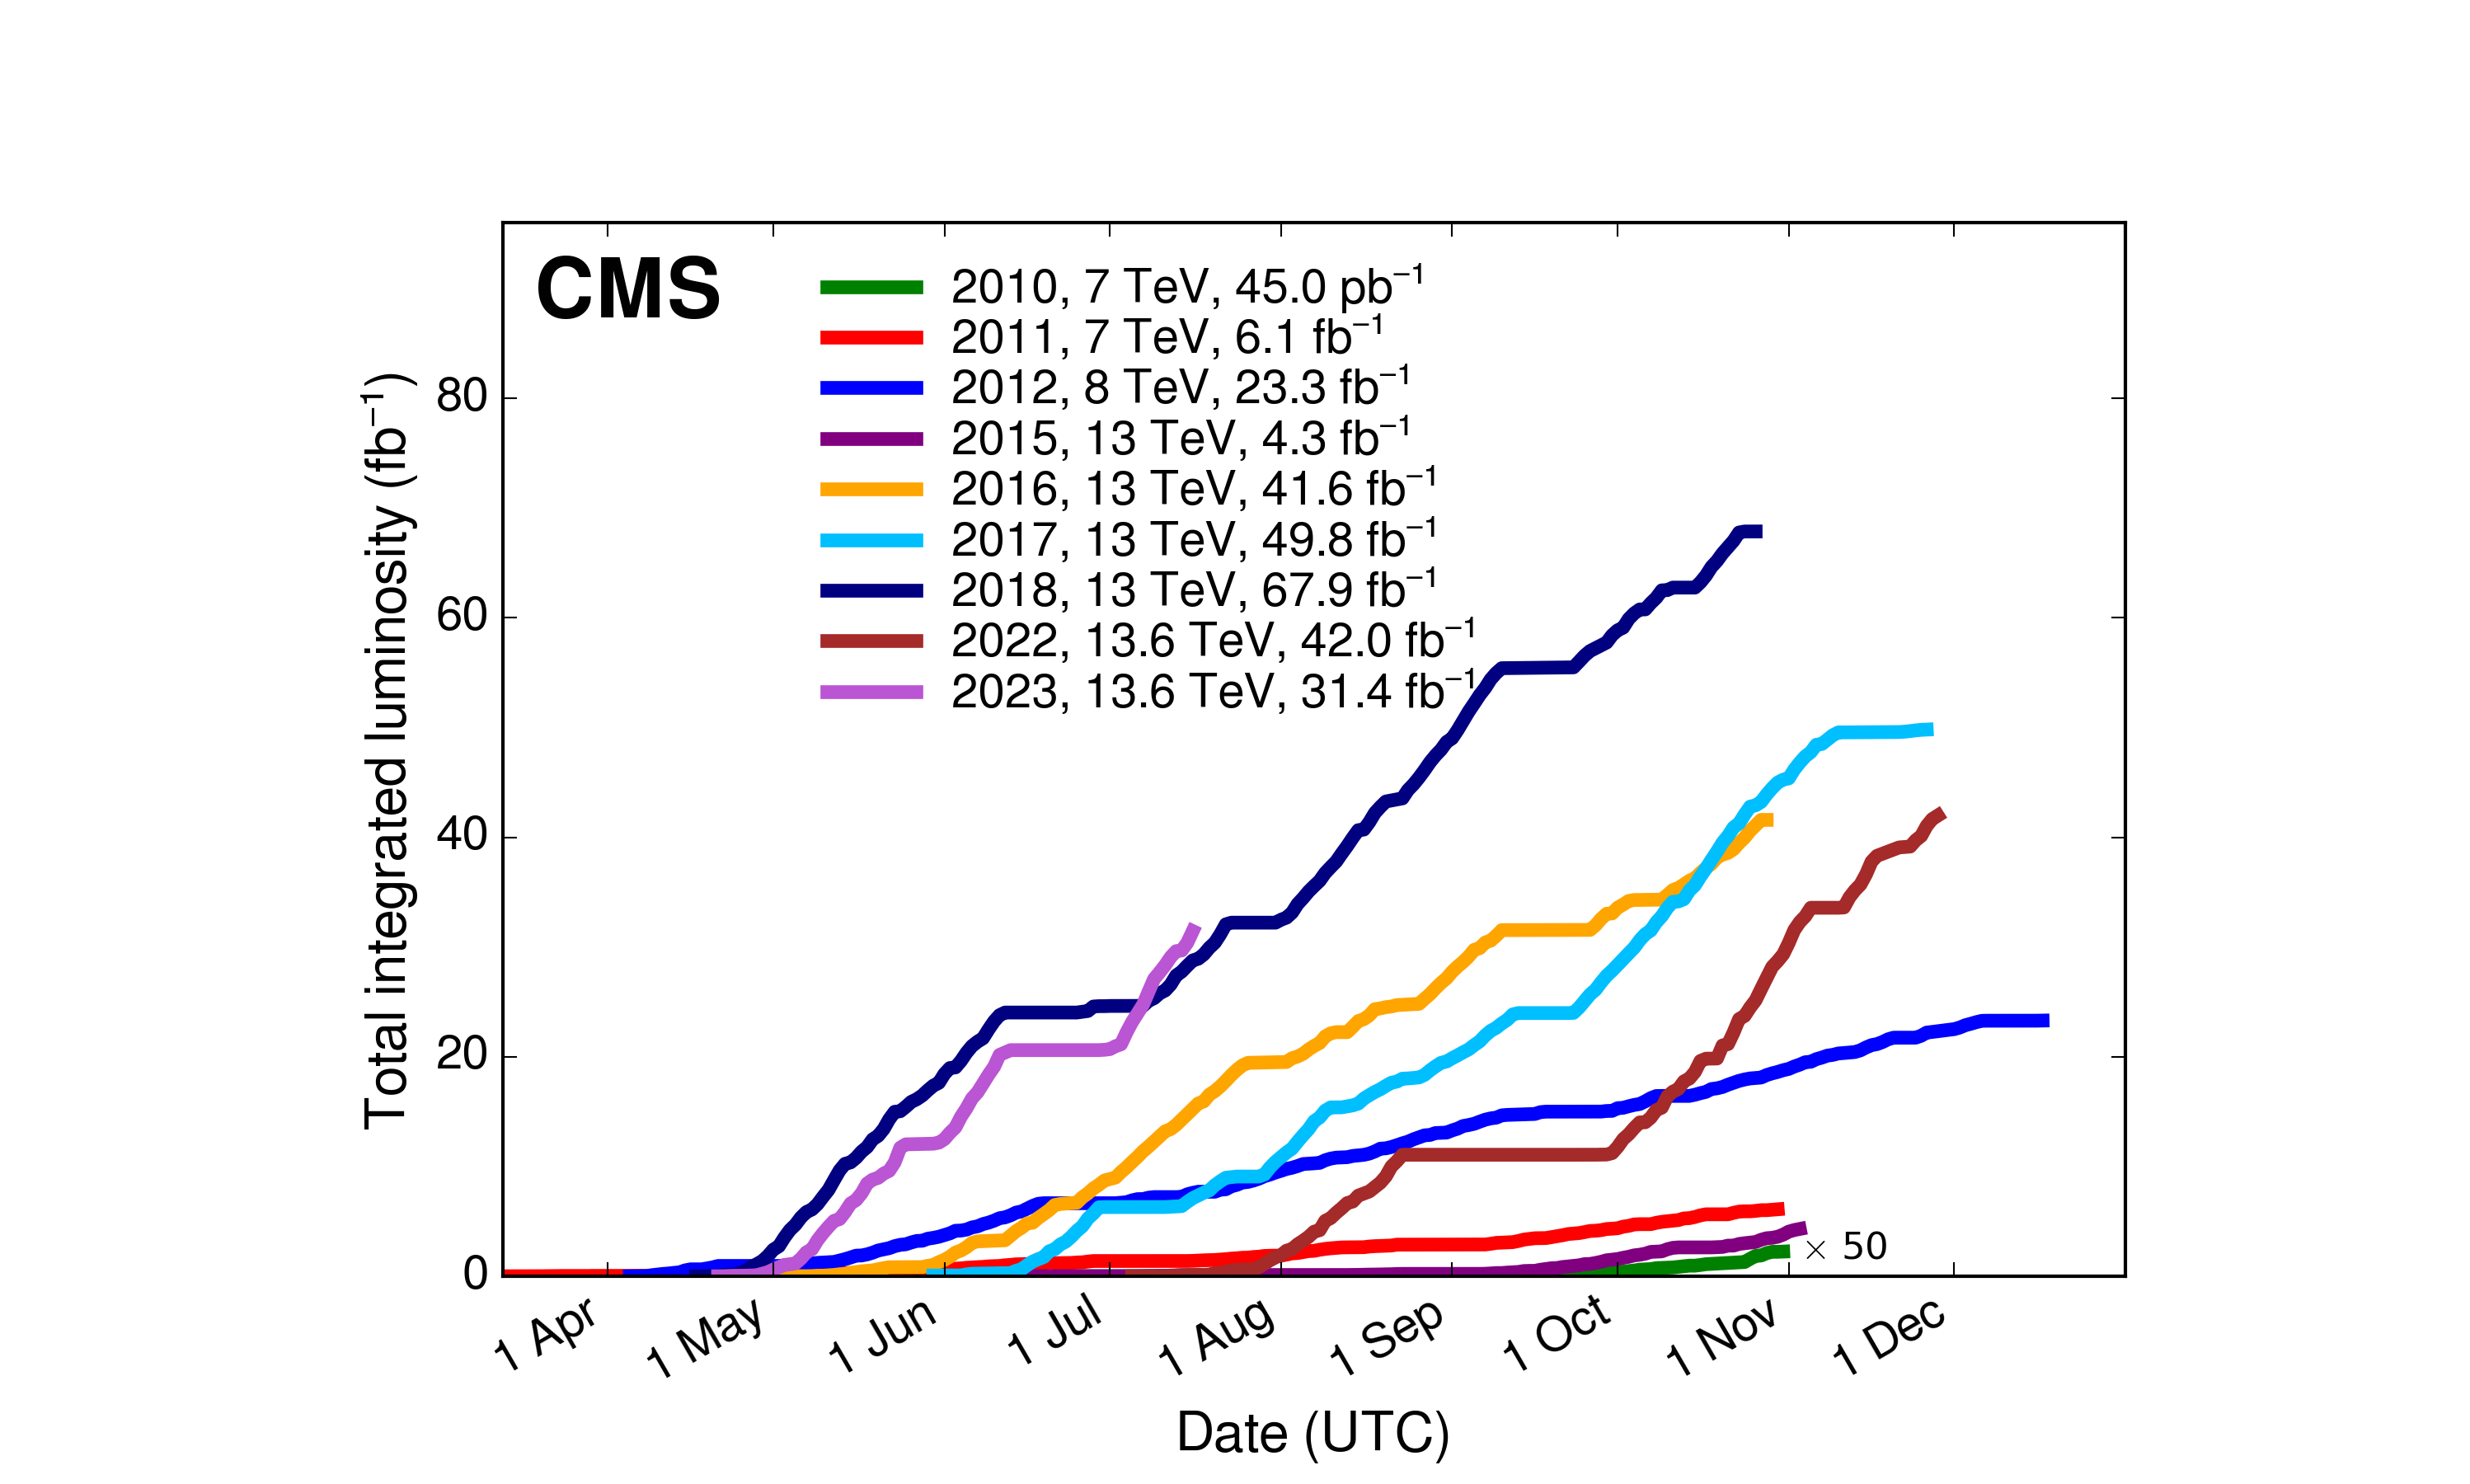
\includegraphics[width=0.48\textwidth]{figures/Part2/LHC/twikilumi}&
 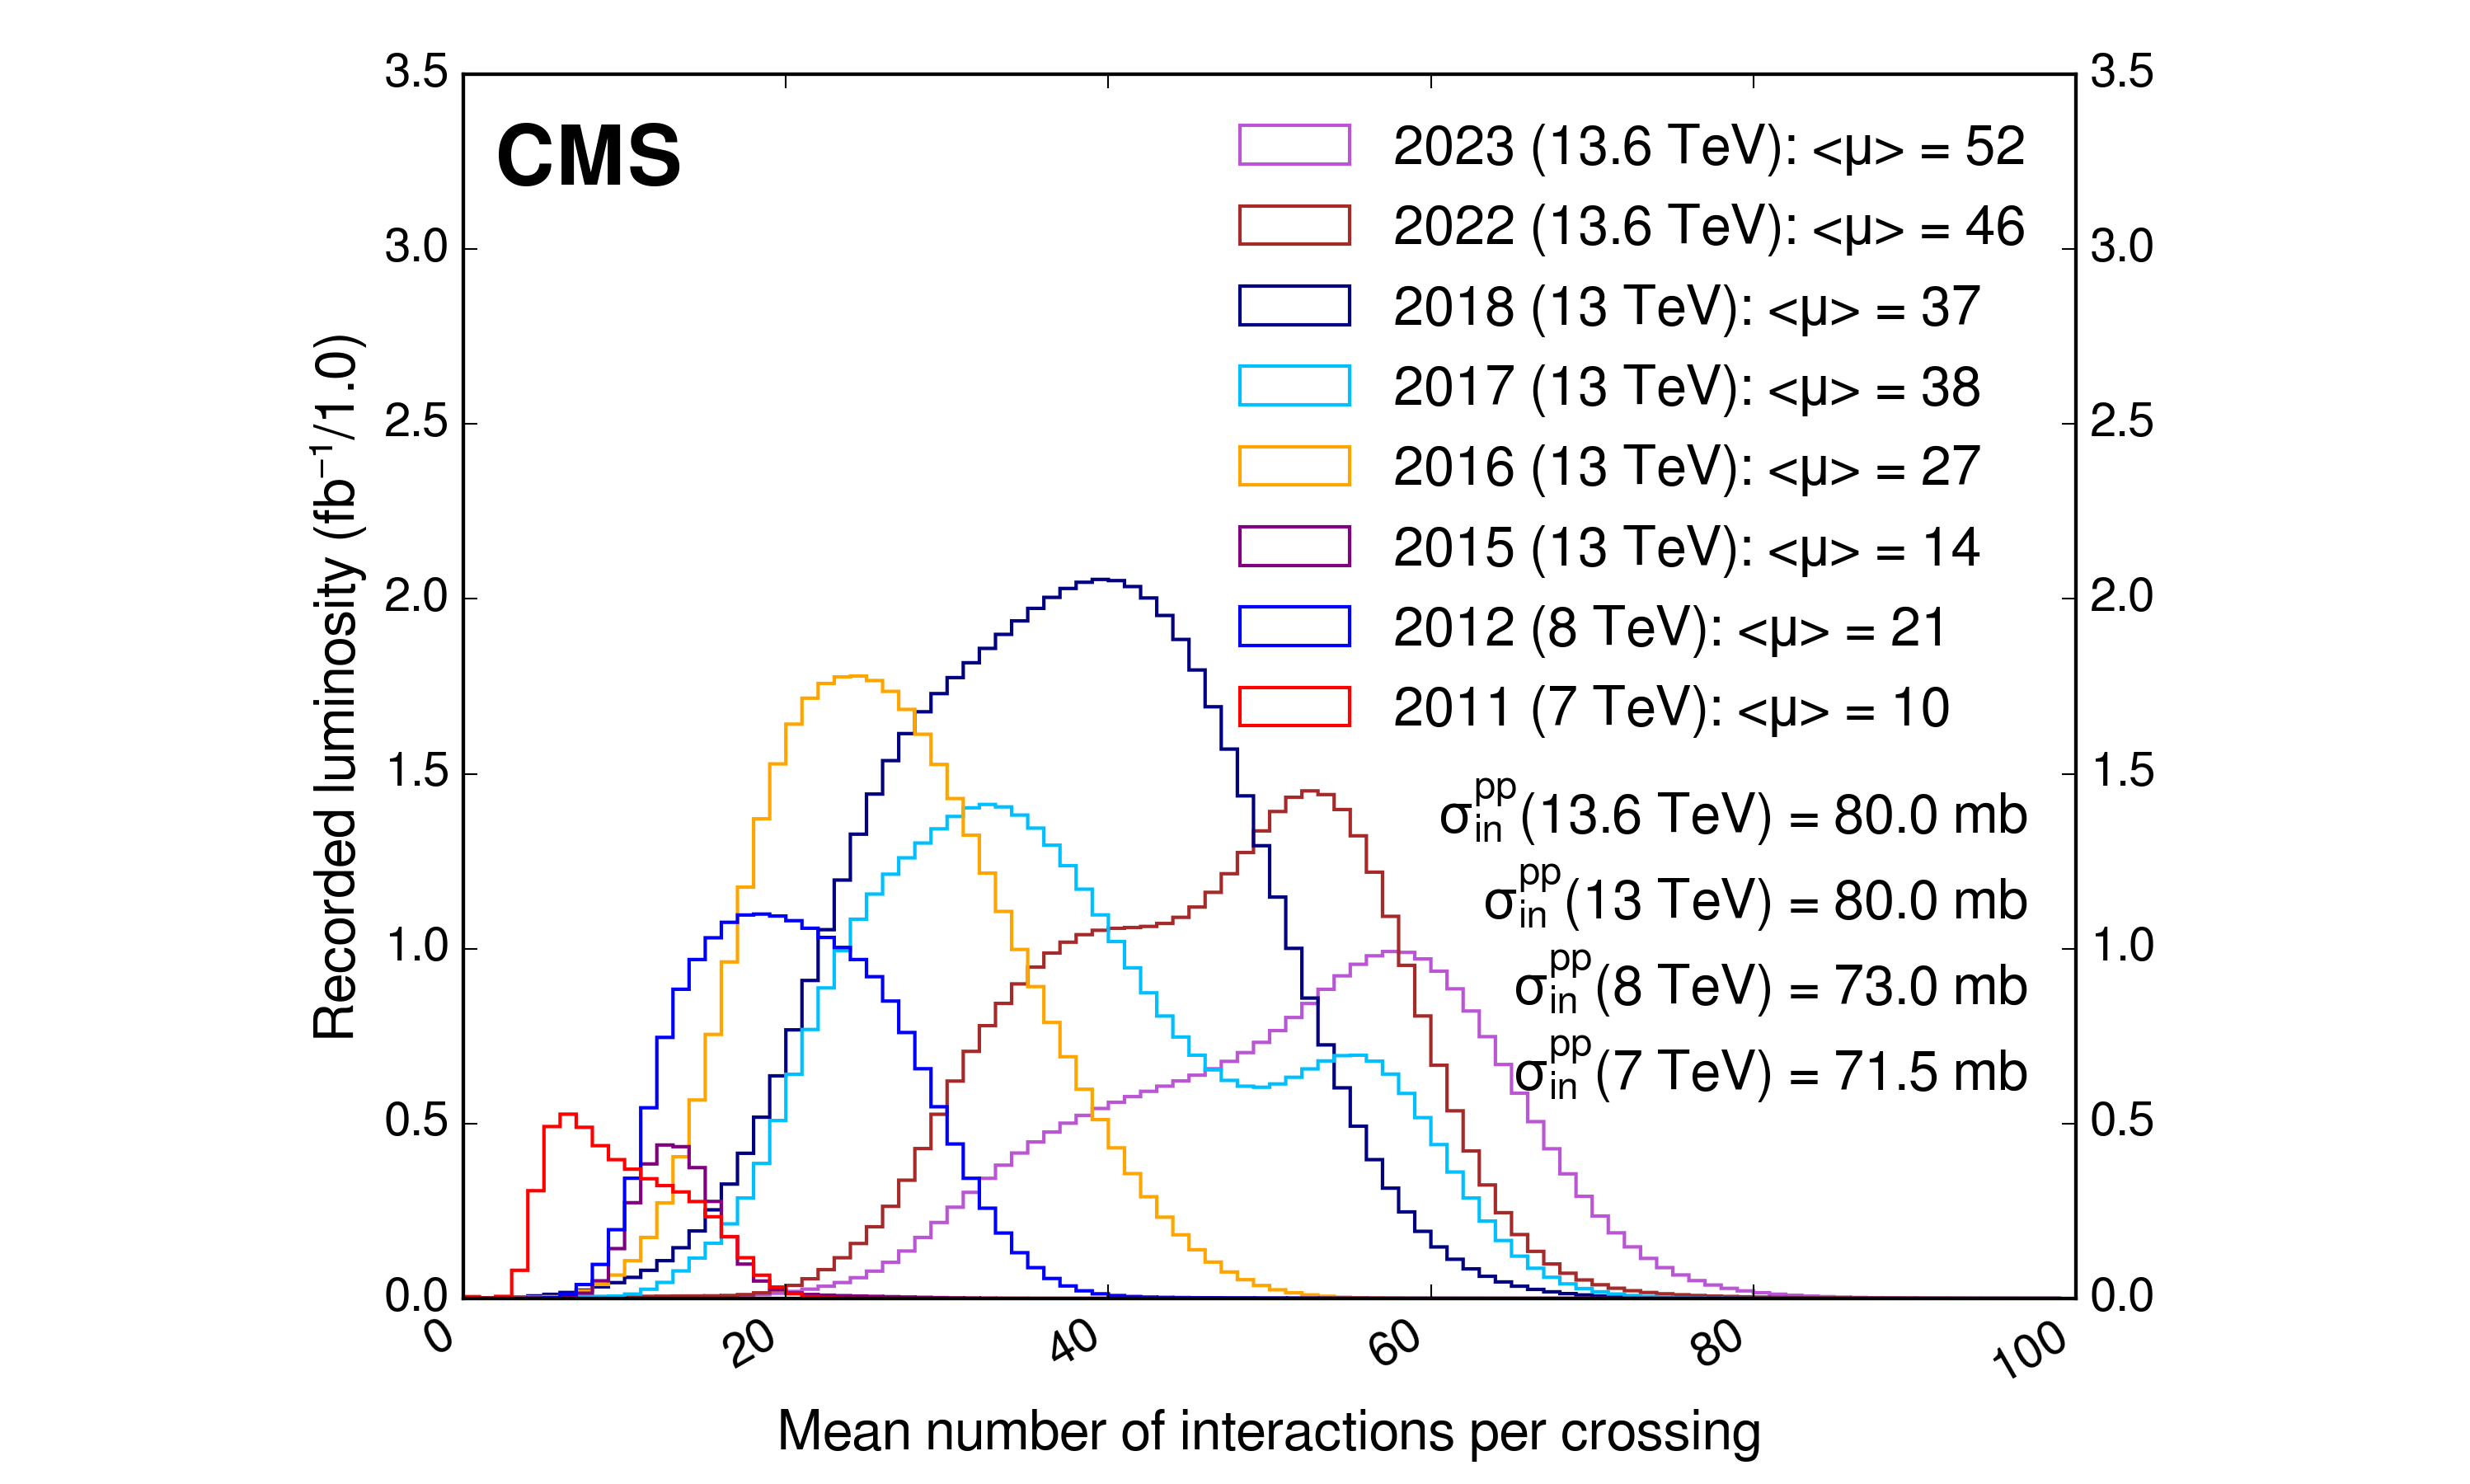
\includegraphics[width=0.48\textwidth]{figures/Part2/LHC/twikipu}\\
 \end{tabular}
 \caption{Delivered integrated luminosity versus time (left) and recorded luminosity versus mean number of interactions per crossing (left), taken from~\cite{twiki:lumi}.}
 \label{fig:twikilumi}
 \end{center}
\end{figure} 

\section{LHC Long Term Schedule}
\label{sec:Plan}

The Long Shutdown 2 (LS2) lasted for over 3 three years until the \ac{LHC} resumed data taking in mid 2022. The on-going run of the \ac{LHC}, known as Run-3, is expected to end in 2025. Between 2026 and 2028 is a period known as the Long Shutdown 3 (LS3), when major upgrades of the \ac{LHC} and the hosted experiments will take place. A new era of the \ac{LHC}, known as the \ac{HL-LHC} will arrive in 2029, when the instantaneous luminosity will gradually increase to up to a factor $7.5$ more than the designed value. The \ac{HL-LHC} is expected to be operational for more than 10 years until the 2040s. A summary of the \ac{LHC} long term schedule is shown in Figure~\ref{fig:Schedule}.

\begin{figure}[tbh!]
 \begin{center}
 \begin{tabular}{c}
 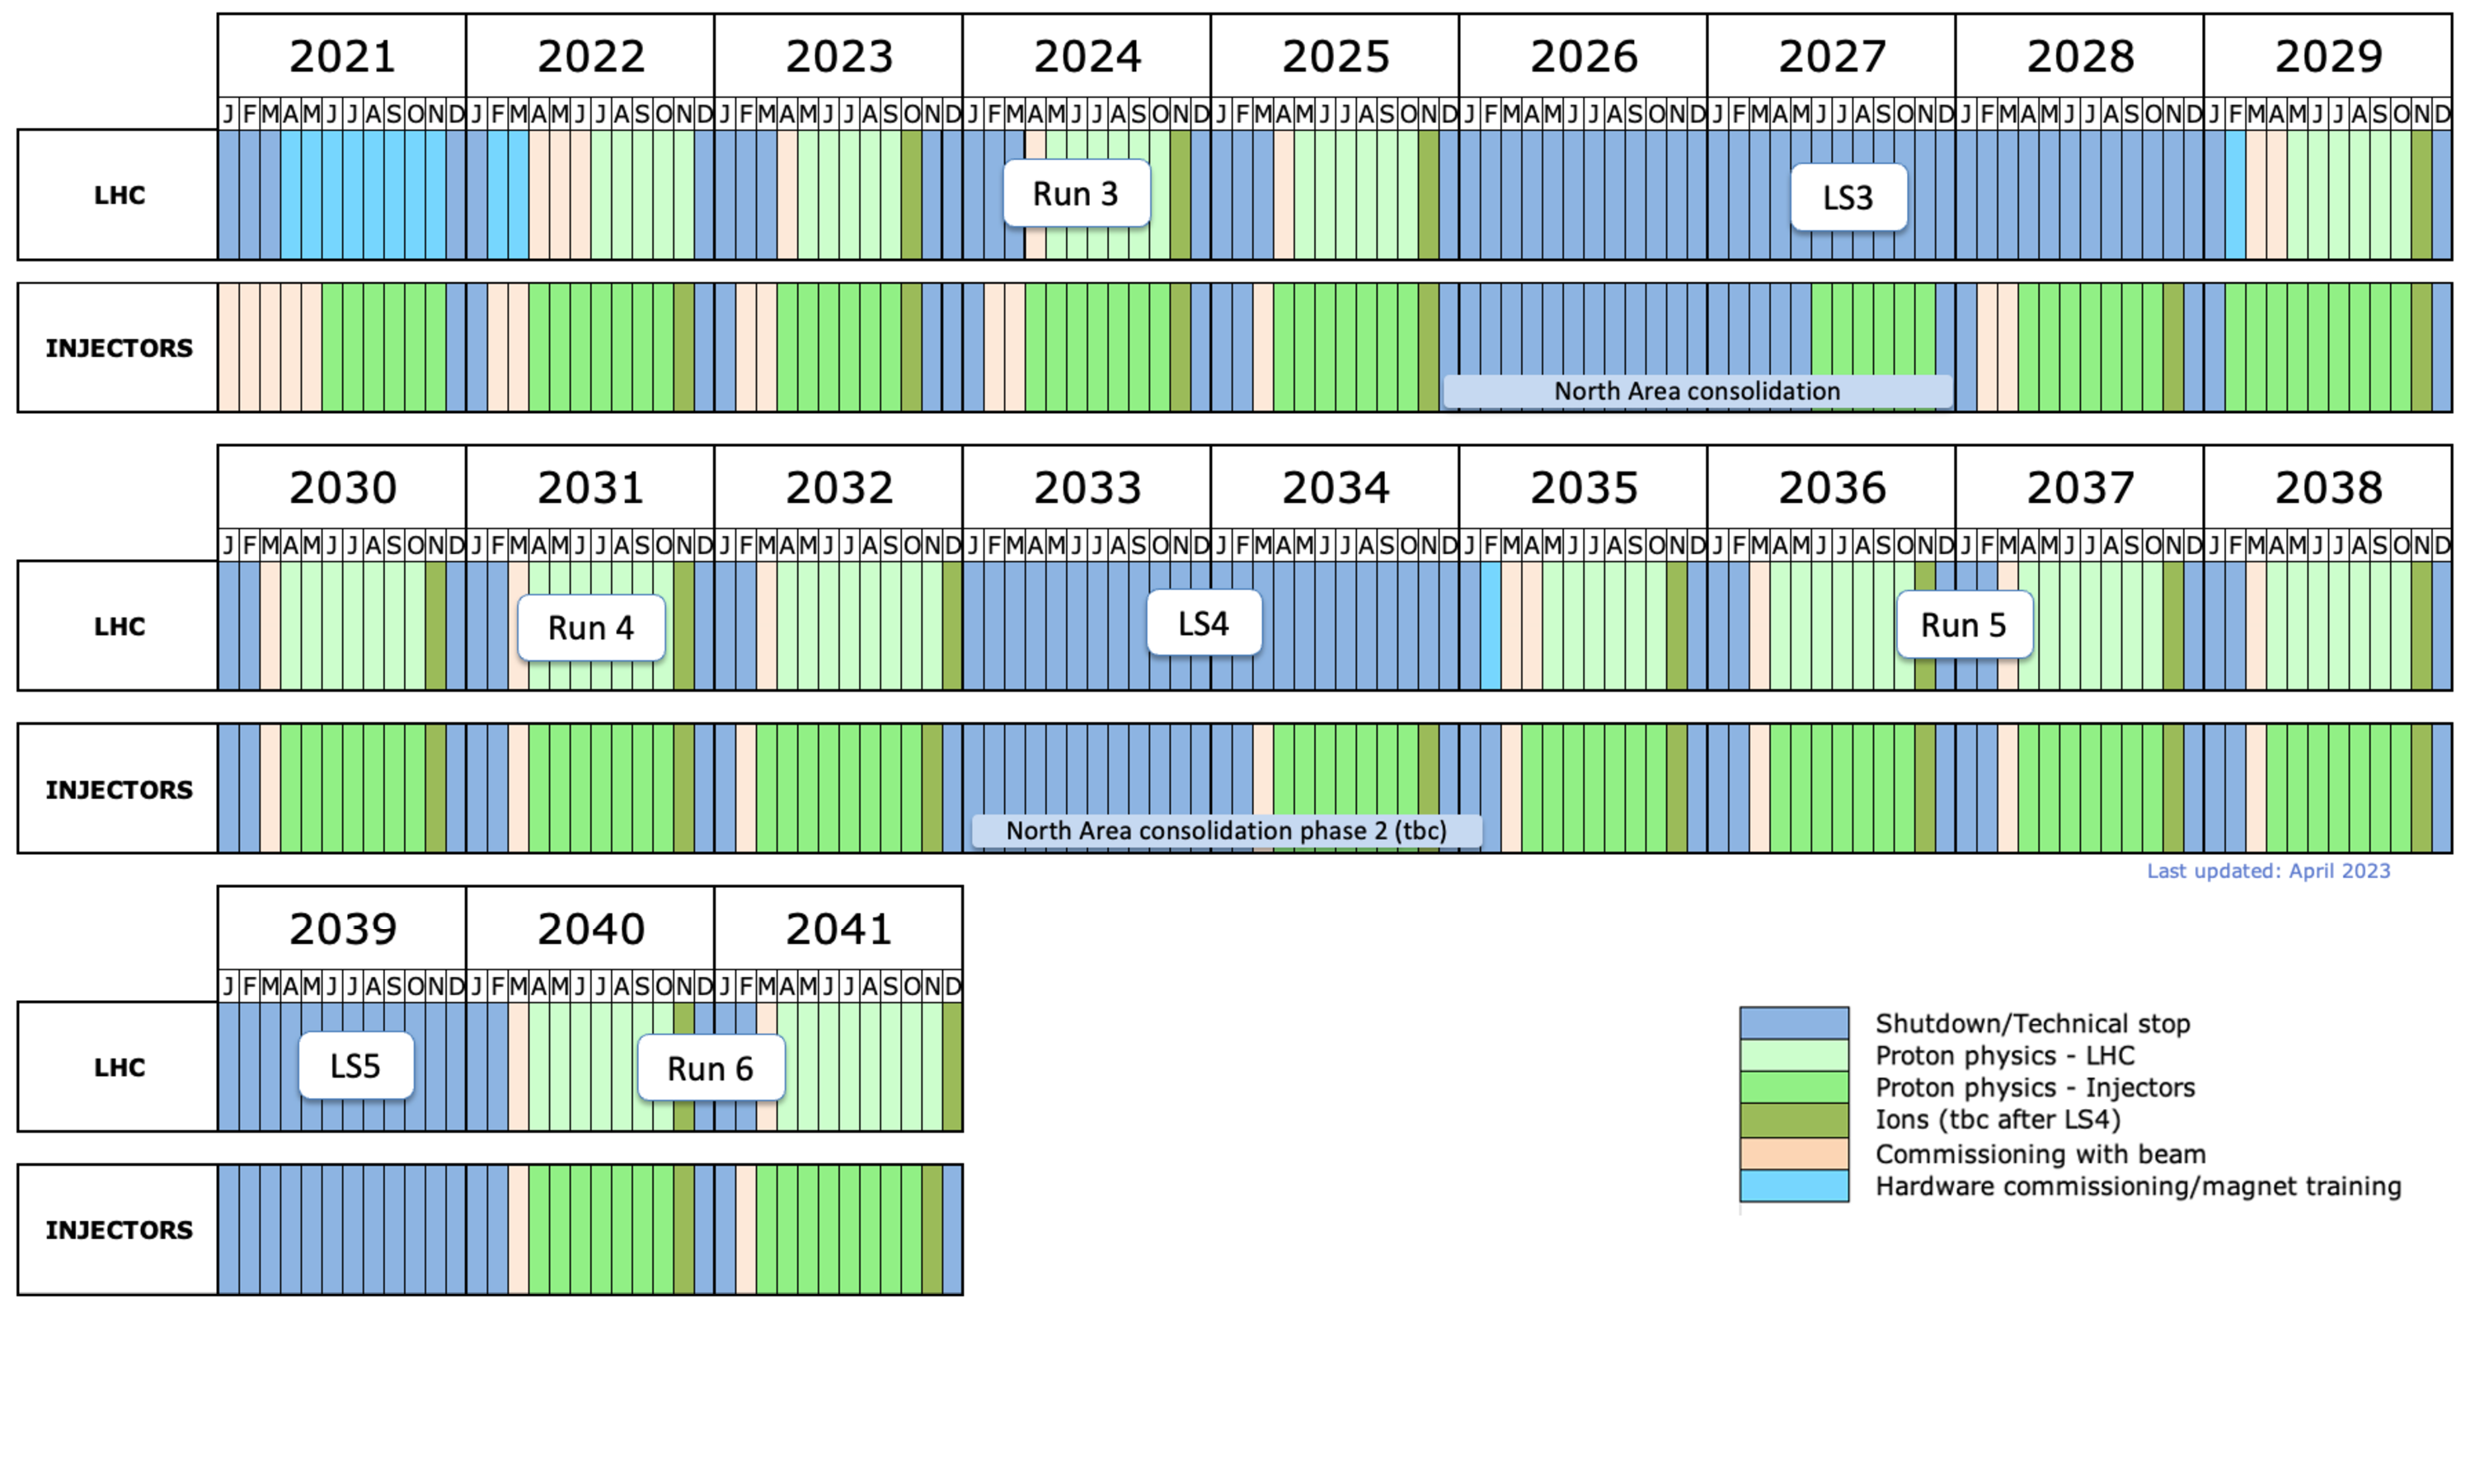
\includegraphics[width=\textwidth]{figures/Part2/LHC/Schedule}
 \end{tabular}
 \caption{The long term schedule of the \ac{LHC}, taken from~\cite{LHC:plan} in November 2023.}
 \label{fig:Schedule}
 \end{center}
\end{figure}
\chapter{The Compact Muon Solenoid Detector}
\label{chap:CMS}

The \ac{CMS} detector~\cite{CMS:2008xjf} is one of the two general-purpose detectors involved in the discovery of the Higgs boson in 2012~\cite{ATLAS:2012yve,CMS:2012qbp}. It is located around 100 meters underground near the French town of Cessy. The full detector weights over 14 thousand tones, and is roughly cylindrically symmetric with a length and diameter of 21 and 15 meters, respectively. It consists of several layers of subsystems, as illustrated in Figure~\ref{fig:CMS}.

\begin{figure}[tbh!]
 \begin{center}
 \begin{tabular}{c}
 \includegraphics[width=0.8\textwidth]{figures/Part2/CMS/cms}
 \end{tabular}
 \caption{A sectional view of the \ac{CMS} detector, adapted from~\cite{Sakuma:2013jqa}.}
 \label{fig:CMS}
 \end{center}
\end{figure}

Brief descriptions of these subsystems are given in \autoref{sec:TK}-\autoref{sec:TrigSys}. The coordinate system adopted by \ac{CMS} is introduced in \autoref{sec:Coord}.

\section{Coordinate System Used in the CMS Detector}
\label{sec:Coord}

As illustrated in Figure~\ref{fig:axis3D}, the coordinate system adopted by \ac{CMS} uses the nominal \ac{IP} as its origin, with the x-axis pointing radially inward towards the center of the \ac{LHC} ring, the y-axis pointing vertically upward towards the sky, and the z-axis pointing along the beam line towards west of the detector.

\begin{figure}[tbh!]
 \begin{center}
 \begin{tabular}{c}
 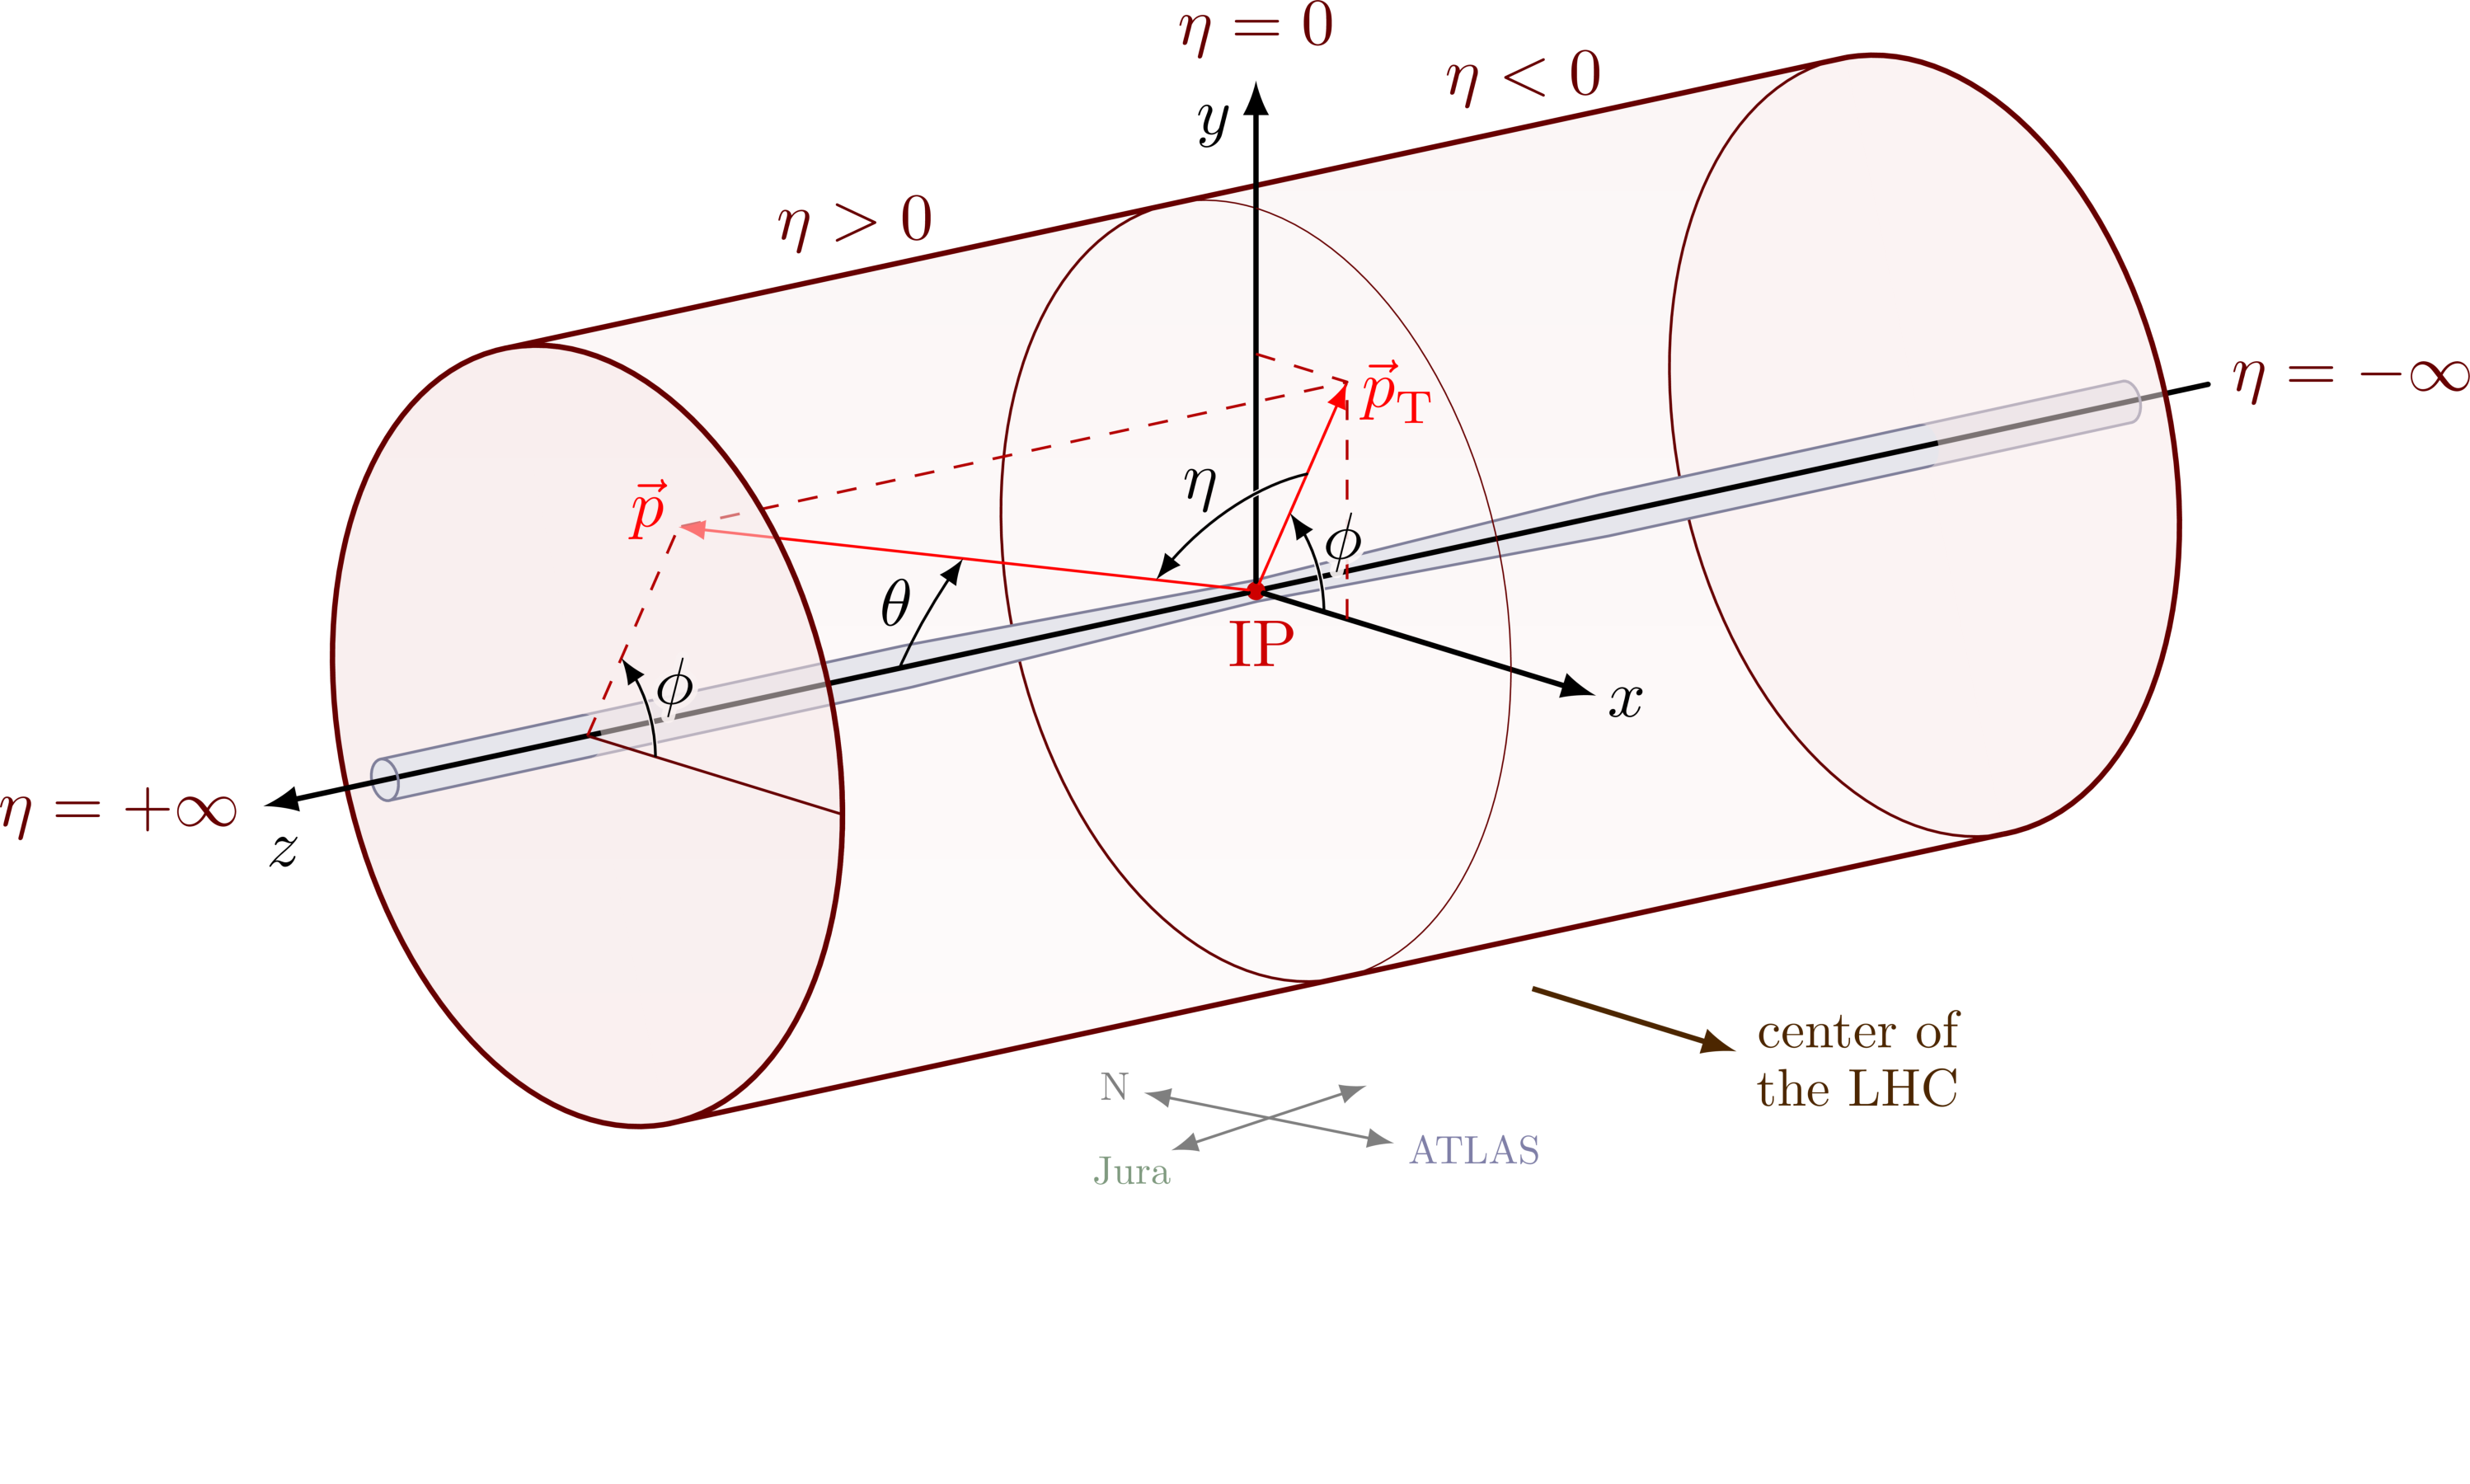
\includegraphics[width=0.8\textwidth]{figures/Part2/CMS/axis3D_CMS-004}
 \end{tabular}
 \caption{A sketch of the coordinate system adopted by \ac{CMS}, adapted from~\cite{tikz:3D}.}
 \label{fig:axis3D}
 \end{center}
\end{figure}

The x- and y-axis form the transverse plane as they are both orthogonal to the beam line (z-axis). The distance from the \ac{IP} in the transverse plane is defined as $r=\sqrt{x^2+y^2}$. Variables defined entirely in the transverse plane, such as $\pt$, \MET, and $\Ht$, are often indicated by a subscripted T. The azimuthal angle $\phi$ is measured from the positive x-axis and the polar angle $\theta$ is measured from the positive z-axis. Another variable $\eta$, known as pseudorapidity, is defined as

\begin{equation}
\eta=-\ln(\frac{\theta}{2}).
\end{equation}

It is preferred over $\theta$ mainly due to: i) particle production rate is roughly uniform in this variable, and ii) a difference in this variables, denoted by $\mathrm{\Delta}\eta$, is invariant under Lorentz boosts. The conversion between $\eta$ and $\theta$ is illustrated in Figure~\ref{fig:axis2D}. The $\mathrm{\Delta}\eta$ and the difference in azimuthal angles, denoted by $\mathrm{\Delta}\phi$, are used to define the distance parameter $\mathrm{\Delta}R$

\begin{equation}
\label{eq:DR}
\mathrm{\Delta}R=\sqrt{\mathrm{\Delta}\eta^2+\mathrm{\Delta}\phi^2}.
\end{equation}

\begin{figure}[tbh!]
 \begin{center}
 \begin{tabular}{c}
 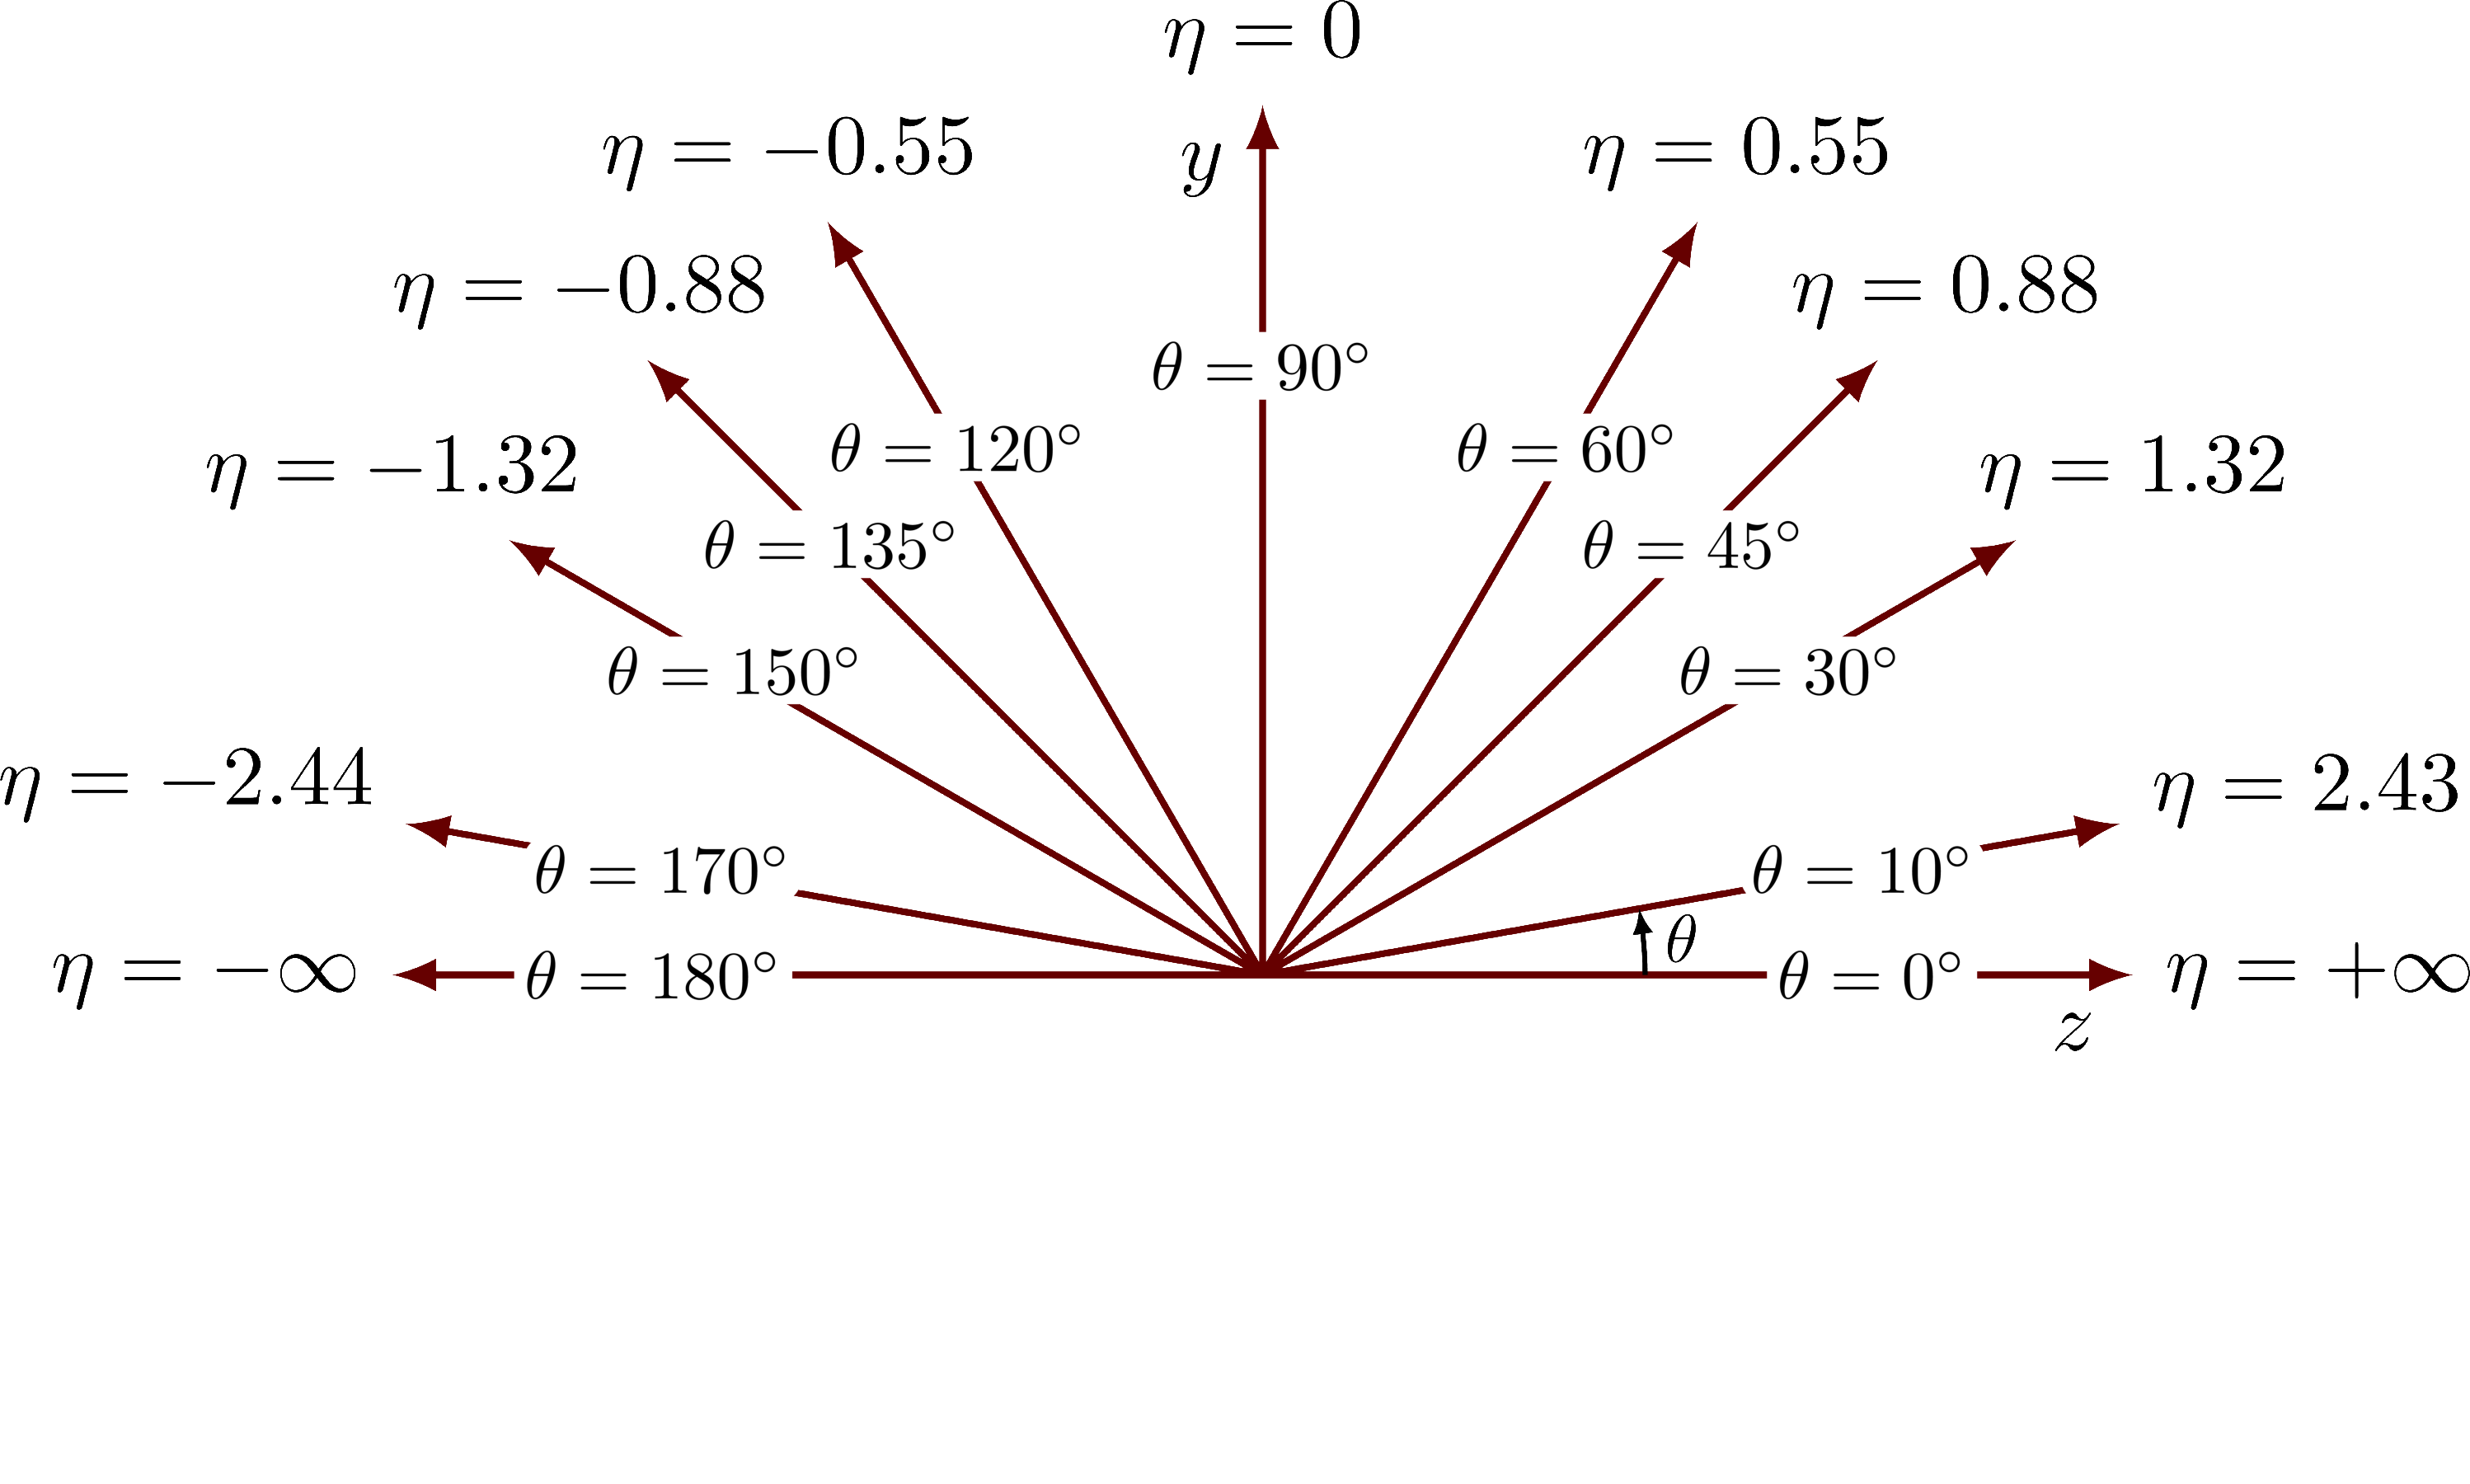
\includegraphics[width=0.8\textwidth]{figures/Part2/CMS/axis2D_pseudorapidity-003}
 \end{tabular}
 \caption{Examples of the conversion between the polar angle $\theta$ and the pseudorapidity $\eta$, adapted from~\cite{tikz:2D}.}
 \label{fig:axis2D}
 \end{center}
\end{figure}

\section{The Tracking System}
\label{sec:TK}

The tracking system is the innermost subsystem of the \ac{CMS} detector where the density of particles from the collisions is the highest. 

\begin{figure}[tbh!]
 \begin{center}
 \begin{tabular}{c}
 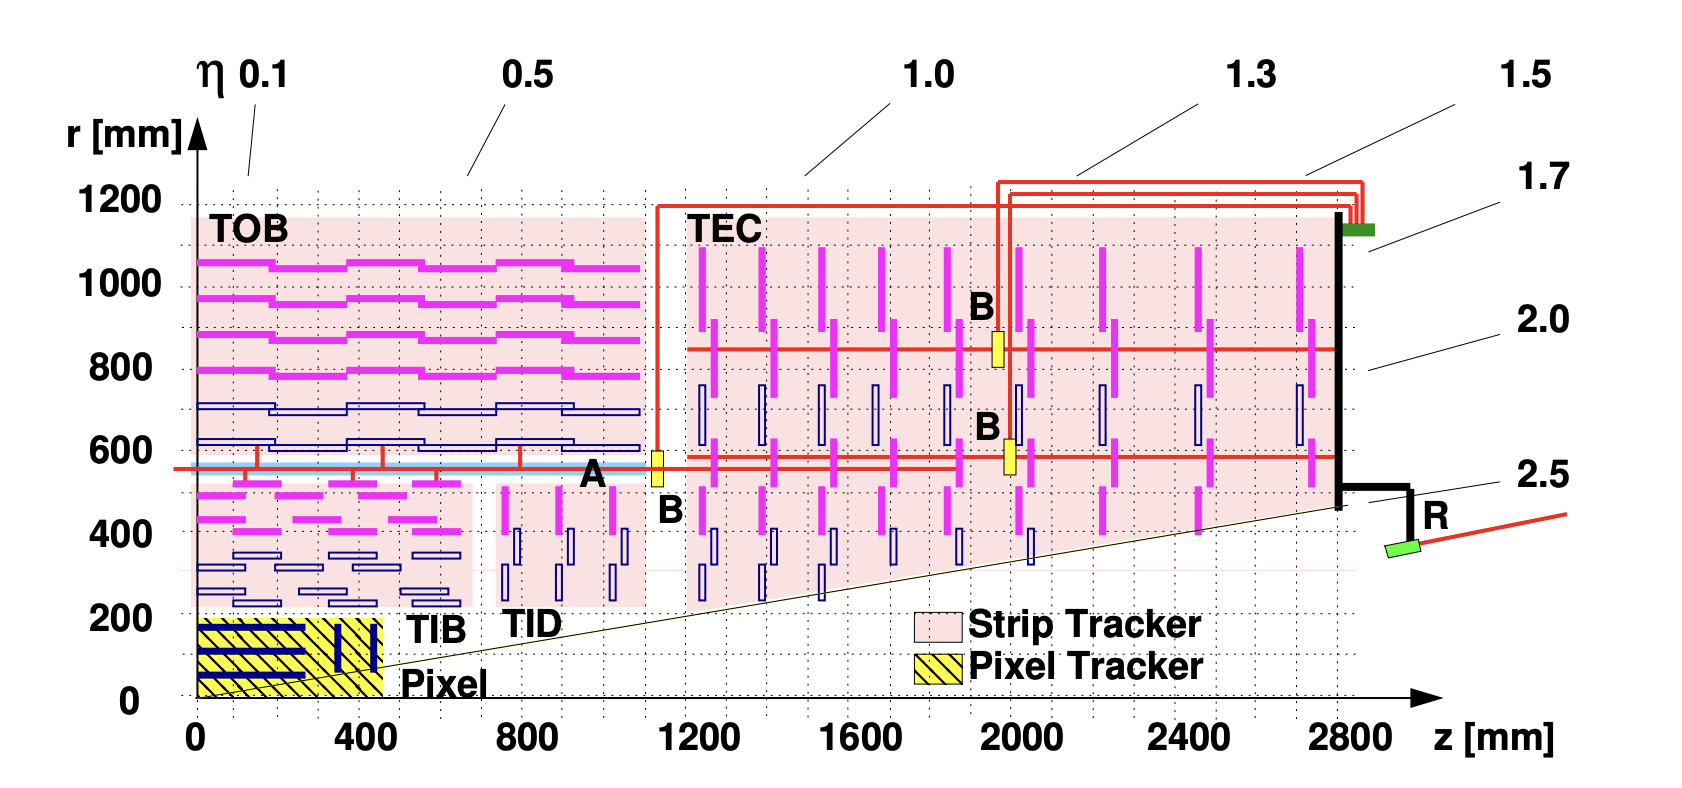
\includegraphics[width=0.8\textwidth]{figures/Part2/CMS/Tracker}
 \end{tabular}
 \caption{A sketch of a quarter of the \ac{CMS} tracker in the $r-z$ plane, adapted from~\cite{CMS:2009dvy}. The strip tracker is shown in pink color, and it is divided into severl parts: the Tracker Inner Barrel (TIB), Tracker Outer Barrel (TOB), Tracker Inner Barrel (TIB), and Tracker Inner Disk (TID). The original pixel detector with three barrel layers is shown in yellow and black colors.}
 \label{fig:Tracker}
 \end{center}
\end{figure}


It uses silicon Pixels and Microstrips to reconstruct the trajectories of charged particles such as electrons and muons, which are then used to determine the momentum as well as the spatial coordinate of these final state particles.

\begin{figure}[tbh!]
 \begin{center}
 \begin{tabular}{c}
 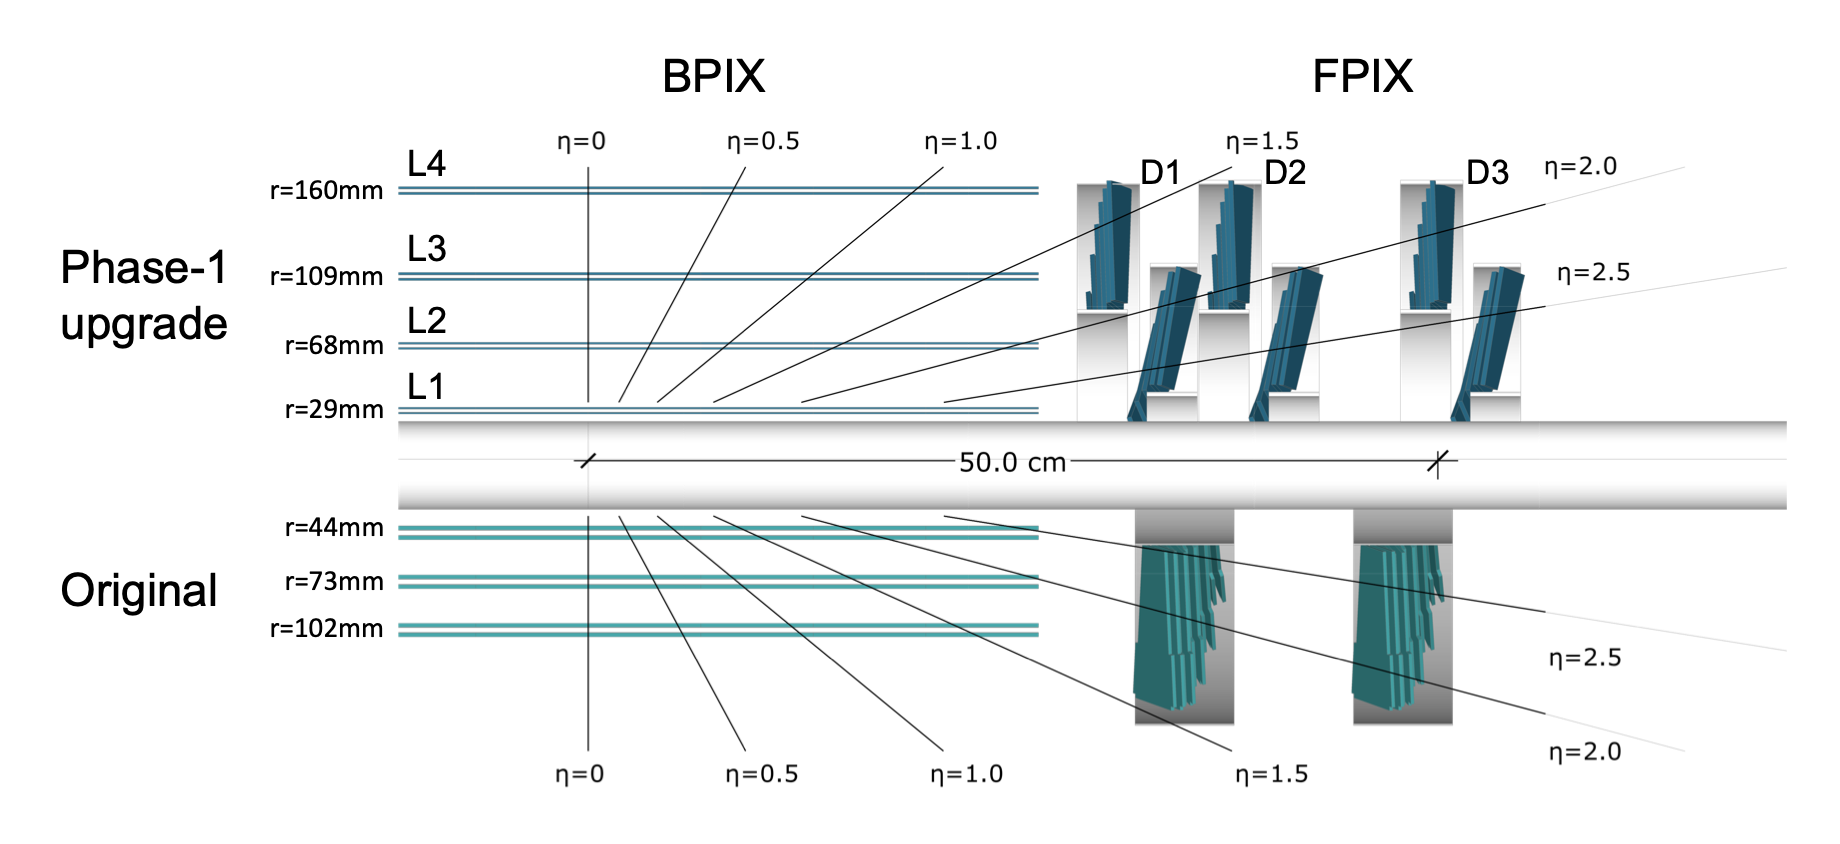
\includegraphics[width=0.8\textwidth]{figures/Part2/CMS/Pixel}
 \end{tabular}
 \caption{A comparison between the original pixel detector and the upgraded pixel detector in the $r-z$ plane, adapted from~\cite{CMSTrackerGroup:2020edz}.}
 \label{fig:Pixel}
 \end{center}
\end{figure}


\section{The Electromagnetic Calorimeter}
\label{sec:ECAL}

The \ac{ECAL} is made of lead tungstate crystals. These dense crystals stop electrons and photons completely and convert their energy into the form of light. The energy of particles can be measured from the intensity of the light.

\section{The Hadronic Calorimeter}
\label{sec:HCAL}

The \ac{HCAL} consists of multiple layers of tiles that form a closed space to ensure high efficiency of missing transverse energy measurement of invisible particles. The tiles stop hadrons completely and transfer the signals to reconstruct the energy and positions of particles.

\section{The Superconducting Magnet}
\label{sec:Magnet}

The superconducting solenoid produces a magnetic field that is close to 4T. The paths of charged particles are curved by this magnetic field in order to identify the charge and momentum of particles. A strong magnetic field is able to curve particles with high energy and provides a good resolution in the high transverse momentum region.

\section{The Muon System}
\label{sec:MuonSys}

The muon detector is the outermost detector of the CMS. The \ac{DT} and \ac{RPC} together make up the barrel region of the muon system, and the end-cap muon system consists of \ac{RPC} and  \ac{CSC}. The \ac{GEM} is the latest addition to the muon system. It complements \ac{CSC} in the forward region. The muon system reconstructs the tracks of muons, and with the strong magnetic field produced by the superconducting solenoid and its iron flux return, the tracks are bent in order to calculate the momentum of muons.

\section{The Trigger System}
\label{sec:TrigSys}

\ac{L1} \ac{HLT} 
\chapter{Event Reconstruction in the CMS detector}
\label{chap:Event}

Events selected by the \ac{CMS} trigger system typically contain signatures of heavy particles, such as the top quark or the Higgs boson. However, the lifetime of these particles is extremely short and they travel a negligible distance before decaying into more stable particles, referred to as the final-state particles. Therefore, the reconstruction of an event produced in the proton-proton collisions requires the identification of all final state particles, which can be then used to infer the presence of heavy particles. Except for weakly interacting neutrinos, all final-state particles leave traces of their signatures in at least one subsystem of the \ac{CMS} detector as illustrated in Figure~\ref{fig:PF}.

\begin{figure}[tbh!]
 \begin{center}
 \begin{tabular}{c}
 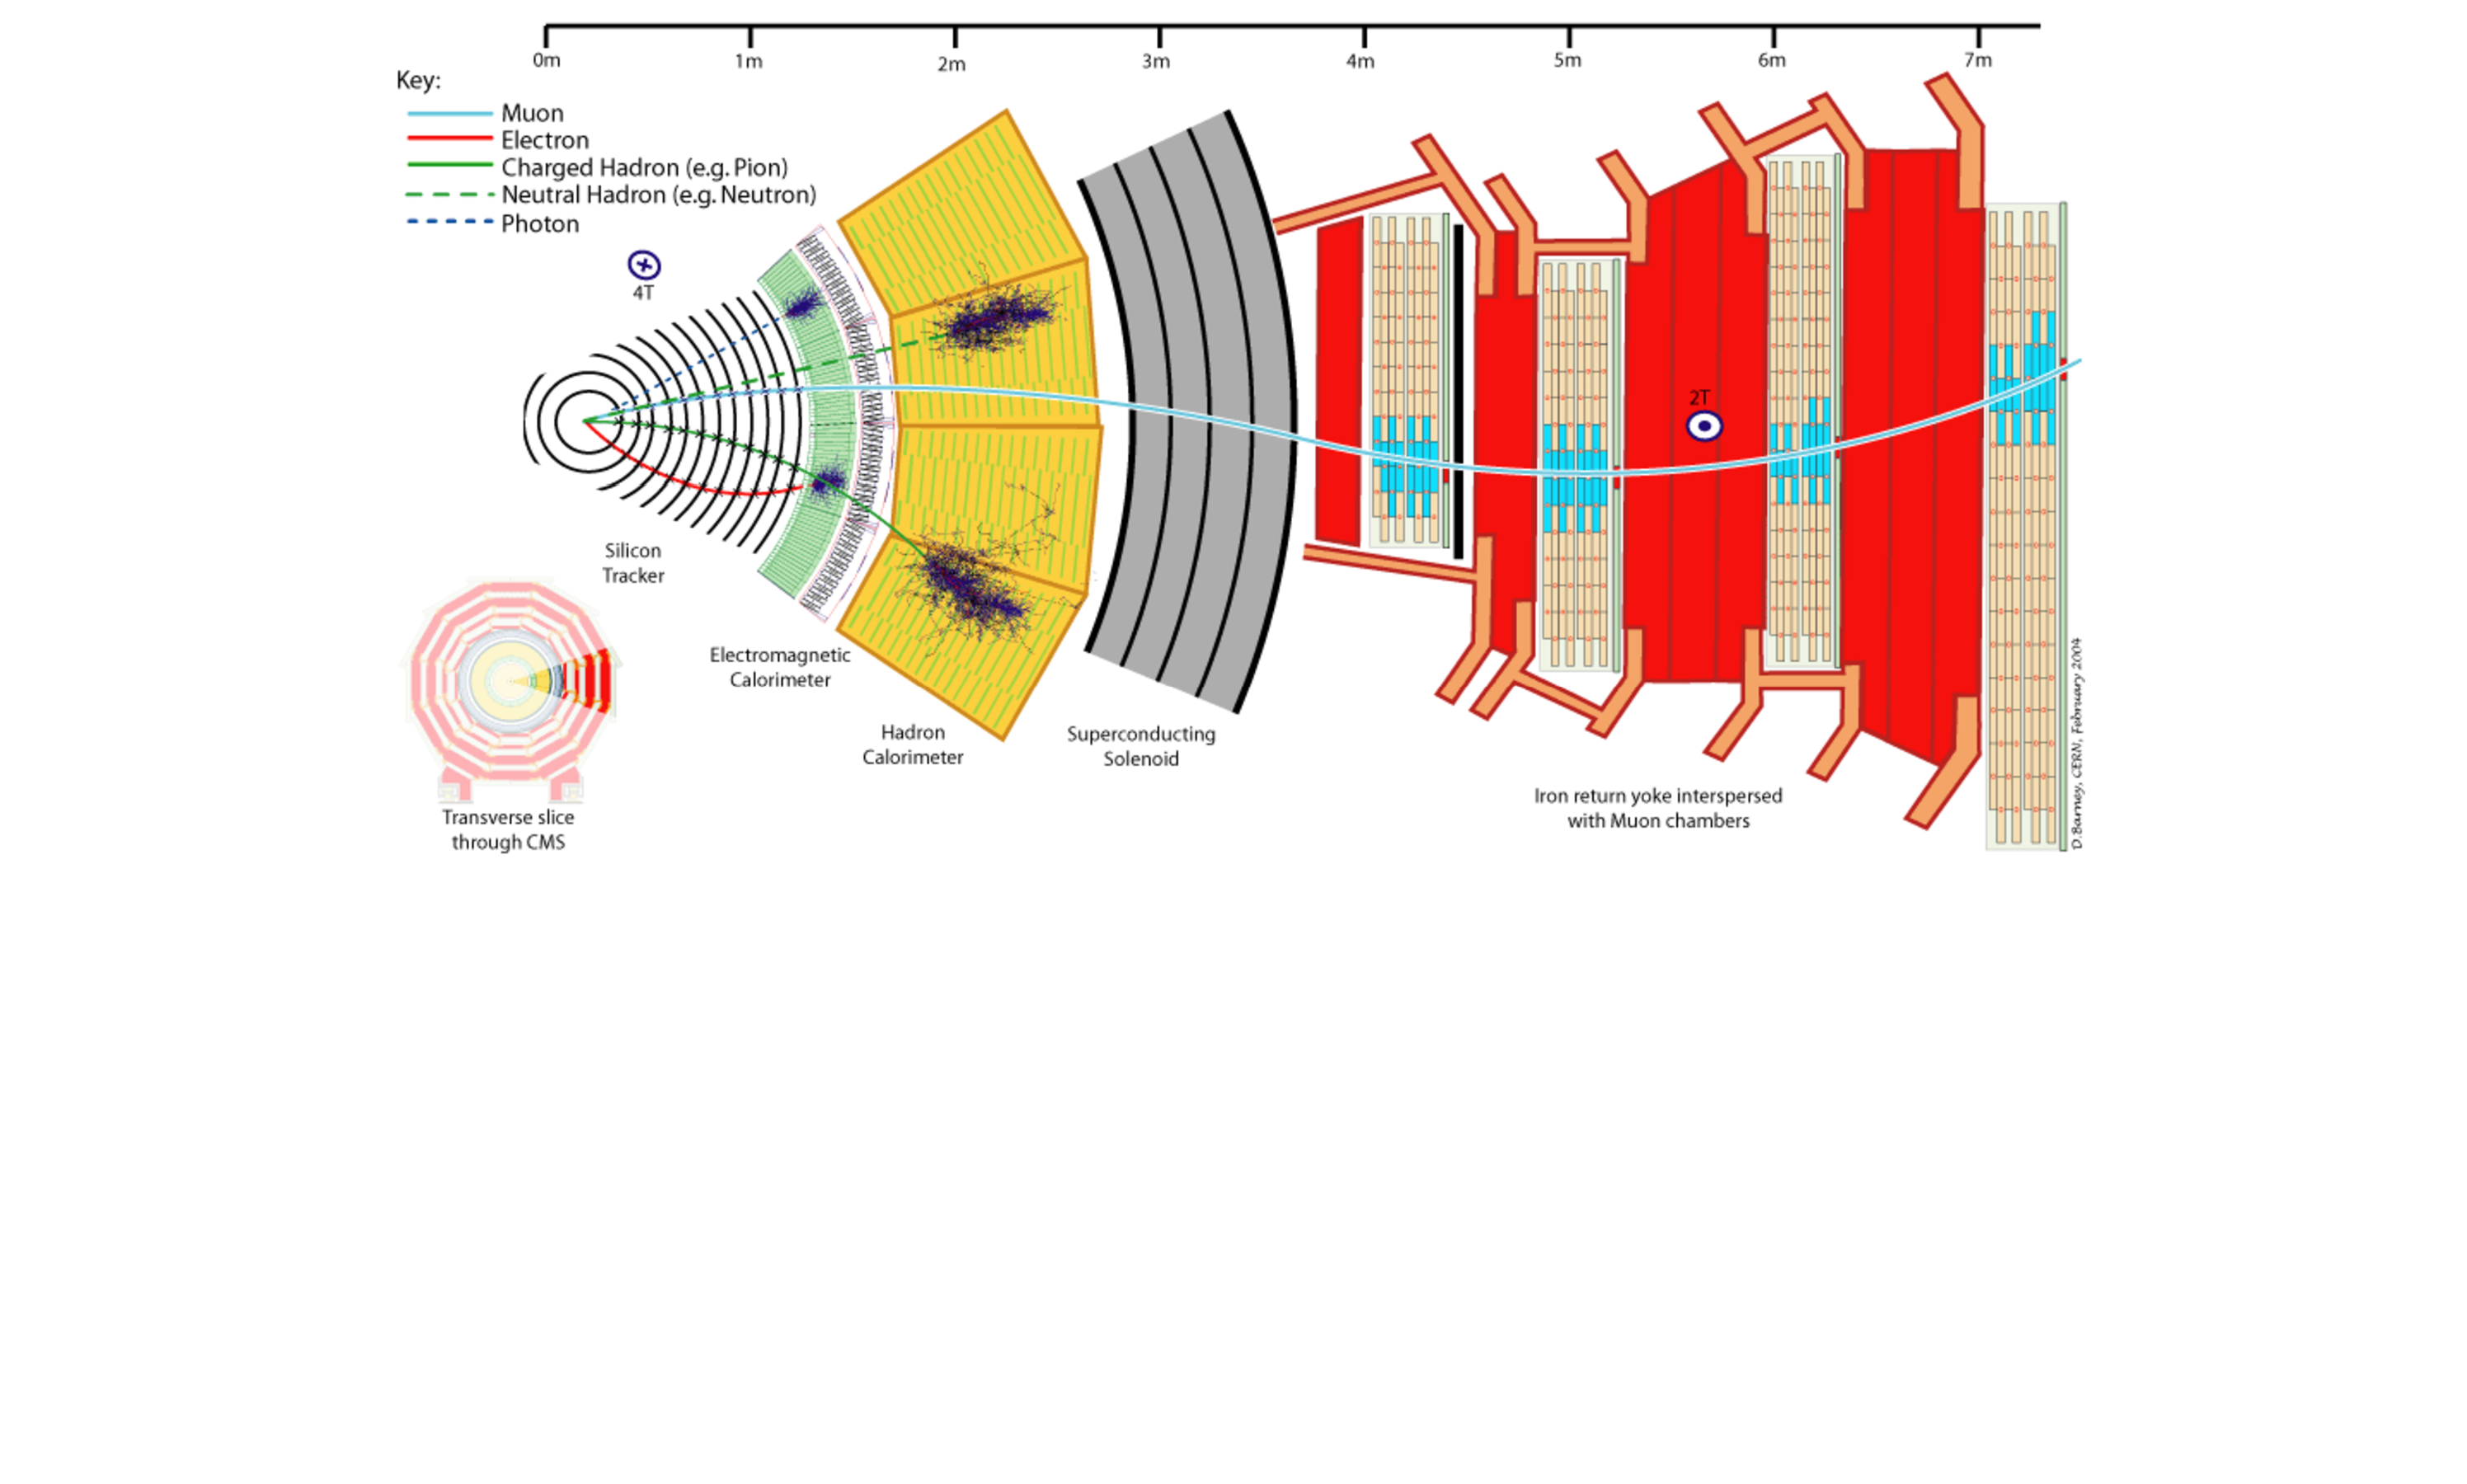
\includegraphics[width=0.9\textwidth]{figures/Part2/Event/PF}
 \end{tabular}
 \caption{A cross-sectional view of a slice of the \ac{CMS} detector in the transverse plane, adapted from~\cite{Barney:2018}. Paths of different particles that interact with various subsystems of the \ac{CMS} detector are highlighted.}
 \label{fig:PF}
 \end{center}
\end{figure}

The \ac{PF} algorithm~\cite{CMS:2017yfk} is used by the \ac{CMS} to combine measurements from all subsystems and provide a global event description. This algorithm consists of two main steps: i) reconstructing the \ac{PF} elements (i.e. tracks and calorimeter clusters) using information from various subsystems and ii) linking these \ac{PF} elements together to form the \ac{PF} candidates. The calorimeter clusters refer to a group of adjacent energy deposits in the calorimeters. The \ac{PF} candidates are labeled as electrons, photons, muons, charged hadrons, or neutral hadrons. Descriptions of the track and vertex reconstruction are given in \autoref{sec:Track}. The reconstruction of \ac{PF} electrons and muons are discussed in \autoref{sec:Electron} and \autoref{sec:Muon}, respectively. The \ac{PF} candidates are also used to reconstruct hadronic jets, taus, and \ac{MET}, which is discussed in \autoref{sec:Jet}, \autoref{sec:Tau}, and \autoref{sec:MET}, respectively.

\section{Track and Vertex}
\label{sec:Track}

Tracks from the inner tracking system and the muon system serve as one of the basic elements of the \ac{PF} algorithm. The standard track reconstruction algorithm at \ac{CMS} is the so-called \ac{CTF}~\cite{Speer:2005dp}, which is an extension of the \ac{KF} algorithm~\cite{Fruhwirth:1987fm} that combines the pattern recognition and parameter fitting. The procedure starts by forming a seed using only two or three hits. The initial estimate of the track parameters and their uncertainties are also made in the seeding stage. A \ac{KF}-based pattern recognition is then used to build track candidates by propagating the trajectory of each seed to its nearby surfaces. If a hit is found in the expected window it is added to the candidate track while the track parameter is updated at the same time. As illustrated in Figure~\ref{fig:CTF}, the improved knowledge of the track parameter as a result of newly added hits allows for a tighter window for the next propagation. 

\begin{figure}[tbh!]
 \begin{center}
 \begin{tabular}{c}
 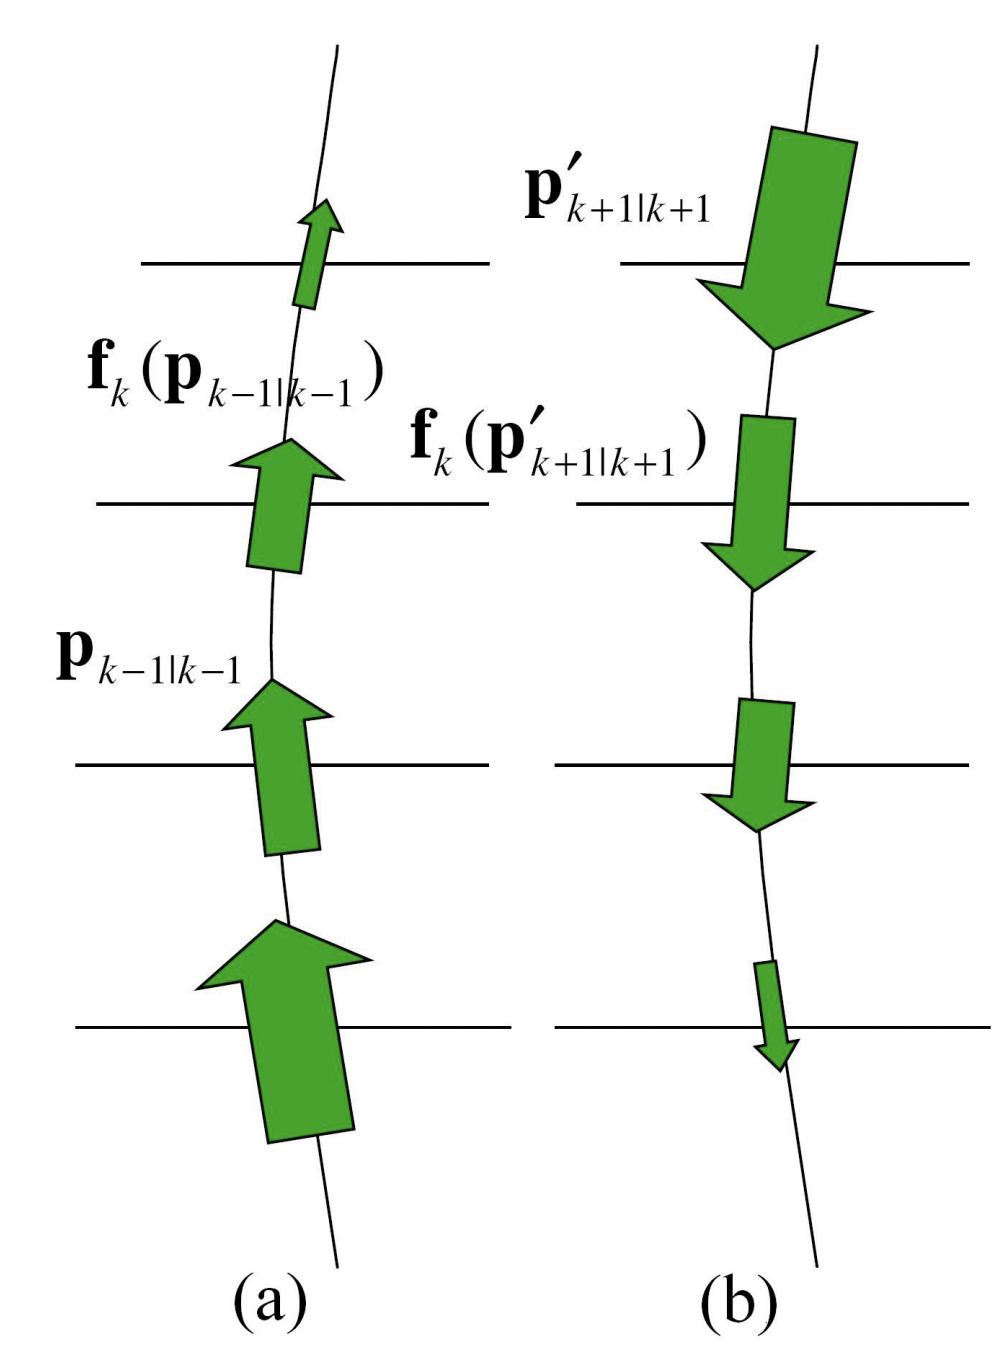
\includegraphics[width=0.4\textwidth]{figures/Part2/Event/CTF}
 \end{tabular}
 \caption{Illustration of the iterative tracking fitting in \ac{CTF}, adapted from~\cite{Lenzi:2008zza}. (a) shows the forward fitting while (b) shows the backward fitting. $\textbf{p}_{k-1|k-1}$ is the \ac{KF} state on surface $k-1$ calculated using the first $k-1$ hits. $\textbf{f}_{k}(\textbf{p}_{k-1|k-1})$ is the predicted \ac{KF} state on surface $k$. The size of the green arrows symbolizes the accuracy of the \ac{KF} state.}
 \label{fig:CTF}
 \end{center}
\end{figure}

The update of the track parameter is done using a \ac{KF} that performs an iterative fit to track parameters as new hits are added. Finally, a set of track quality selection criteria is applied to reduce the number of tracks that can not be associated with any particles, known as fake tracks. 

Reconstructed tracks can also be linked together to form a vertex. Vertices that are associated with inelastic scatterings of a collision event are known as the \ac{PV}. Due to the presence of \ac{PU}, multiple \acp{PV} exist in any given collision event. Three main steps are involved in the reconstruction of the \acp{PV}. Firstly, a set of selection criteria is applied to reconstructed tracks to ensure they are promptly produced in the collisions. Secondly, reconstructed tracks are clustered into a vertex candidate based on their $z$-coordinates using the deterministic annealing algorithm~\cite{Rose:1998dzq}. Finally, candidate vertices with more than one associated track are fitted using adaptive vertex fitter~\cite{Fruhwirth:2007hz}. For each event, the \ac{PV} with the highest $\sum\pt^2$ is often considered to be of the most importance to particle physicists as they carry the largest momentum transfer in an event. It is sometimes referred to as simply the \ac{PV} of an event while other \acp{PV} are considered to originate from \ac{PU}.

\section{Electron}
\label{sec:Electron}

Charged particles may emit photons in a process called the \emph{bremsstrahlung}. The intensity of this effect is inversely proportional to the squared mass of the charged particles. As the lightest charged particles, electrons produced in the hadron collisions are heavily affected by the bremsstrahlung effect, which comes in two different aspects. Firstly, the emission of a photon alters the electron trajectory, which undermines the performance of the standard tracking algorithm. A dedicated algorithm known as the \ac{GSF}~\cite{Adam_2005} is therefore used to fit the electron parameters. Moreover, the bremsstrahlung photons emitted by electrons often cause a more widespread pattern of \ac{ECAL} clusters along the $\phi$ direction. Therefore, multiple adjacent \ac{ECAL} clusters are combined to form the so-called \emph{superclusters}.

The electron reconstruction is fully integrated into the \ac{PF} framework, which associates \ac{GSF} tracks from the inner tracking system to the \ac{ECAL} clusters. The final assignment of the electron energy is based on a weighted combination of the \ac{ECAL} super cluster energy and tracker momentum~\cite{Baffioni:2006cd}. In addition to the electron reconstruction, identification criteria are often applied and optimized for different analyses. For both analyses described in this thesis, the primary objective of the electron identification is to control the contamination of the \emph{nonprompt} leptons. To this end, a \ac{BDT}-based electron identification is deployed, which is discussed in \autoref{sec:Leptons}.

\section{Muon}
\label{sec:Muon}

In \ac{CMS}, three types of muon tracks exist: standalone muons, tracker muons, and global muons~\cite{CMS:2018rym}. The standalone muons refer to the muon tracks reconstructed purely from hits in the muon system. The tracker muons are built ``inside-out'' by propagating tracks from the tracker to the muon system and matching it with at least one hit from either the \ac{CSC} or \ac{DT}. The global muon is reconstructed ``outside-in'' by: i) matching the standalone muons with the inner tracks and ii) performing a combined fit using the \ac{KF} to update the muon parameters. 

Same as the electron, the muon reconstruction is fully integrated into the \ac{PF} algorithm, which applies a set of selection criteria based on quality parameters in the muon reconstruction to the tracker muons and global muons. The so-called Medium muon ID~\cite{CMS:2018rym} is used by analyses described in this thesis. This ID accepts both tracker muons and global muons and adjusts the selection criteria accordingly. The overall efficiency of this ID is estimated to be around 99.5\% for muons from simulated W and Z events.

\section{Jet}
\label{sec:Jet}

The \ac{CMS} uses a sequential recombination algorithm, known as the anti-$k_t$ algorithm~\cite{Cacciari:2008gp}, to cluster \ac{PF} candidates into jets. The word ``$k_t$'' refers to the transverse momentum. This algorithm is designed to be \ac{IRC} safe, meaning the jet properties are invariant under the soft gluon emissions and collinear gluon splitting. The distance variable between two \ac{PF} candidates $i$ and $j$ in this algorithm is defined by 

\begin{equation}
\label{eq:ak}
d_{ij} = \min(\frac{1}{p_{\textsf{T}_i}^2},\frac{1}{p_{\textsf{T}_j}^2})\frac{\mathrm{\Delta}R_{ij}}{R},
\end{equation}

where $p_{\textsf{T}_i}$ and $p_{\textsf{T}_j}$ corresponds to the transverse momentum of \ac{PF} candidate $i$ and $j$ respectively. $\mathrm{\Delta}R_{ij}$ is the angular distance between the two objects defined by

\begin{equation}
\mathrm{\Delta}R_{ij} = \sqrt{\mathrm{\Delta}y_{ij}^2+\mathrm{\Delta}\phi_{ij}^2},
\label{eq:DDR}
\end{equation}

where $y=\frac{1}{2}\ln(\frac{E+p_z}{E-p_z})$, referred to as the rapidity, is not to be confused with the pseudorapidity $\eta$ defined in Equation~\ref{eq:eta}. $R$ in Equation~\ref{eq:DDR} denotes the size of the jet which is typically chosen to be smaller than 1. A second variable that measures the distance between particle $k$ and the beam axis in momentum space is defined as 

\begin{equation}
d_{kB} = \frac{1}{p_{\textsf{T}_k}^2}.
\end{equation}

The recombination procedure begins with calculating all combinations of $d_{ij}$ and concatenating them with every $d_{kB}$ to form the set $\{d_{ij}\}\cup\{d_{kB}\}$. The minimum of the entire set is then determined. If $d_{ij}$ is the minimum, then \ac{PF} candidates $i$ and $j$ are recombined into one candidate which replaces candidate $i$ and $j$ in the list. If $d_{kB}$ is the minimum, then it is labeled as a jet and removed from the list. This process is iterated until no \ac{PF} candidates are left. The name ``anti-$k_t$'' refers to the fact that the distance variable $d_{ij}$ is defined with respect to $k_t$ to the power of -2, which is different from the use of $k_t^2$ in $k_t$ algorithm~\cite{Ellis:1993tq}. 

As indicated in Equation~\ref{eq:ak}, the anti-$k_t$ algorithm is dominated by hard particles. It typically starts with the hardest particle in an event and clusters and walks its way down to softer particles. The final momentum assignment of a jet is determined by the vectorial sum of the momenta of all particles that are clustered into this jet. The softest particles in an event are typically among the last ones to be clustered and they do not affect hard jets. The infrared safety is therefore guaranteed. Moreover, two collinear particles will also be given high priority to be merged because of the small $d_{ij}$ between them. This effectively ensures the collinear safety of the algorithm. Historically, sequential clustering algorithms are favored by theorists because of their \ac{IRC} properties but not favored by experimentalists due to their computational complexity. The introduction of the \textsc{FastJet} program~\cite{Cacciari:2011ma} improves significantly the the running speed of these sequential clustering algorithms, and they eventually become the standard jet clustering algorithm at the \ac{LHC}.

The measured energy of a jet is calibrated by applying a multiplicative factor $\mathcal{C}$ to each of its four-momentum components:

\begin{equation}
p^{\textsf{corr}}_{\mu} = \mathcal{C}\cdot p^{\textsf{raw}}_{\mu},
\end{equation}

where $\mathcal{C}$ is factorized into several components~\cite{CMS:2011shu},

\begin{equation}
\mathcal{C} = \mathcal{C}_{\textsf{offset}}(\pt^{\textsf{raw}})\cdot\mathcal{C}_{\textsf{MC}}(\pt^{\prime},\eta)\cdot\mathcal{C}_{\textsf{rel}}(\eta)\cdot\mathcal{C}_{\textsf{abs}}(\pt^{\prime\prime})
\end{equation}

where $\mathcal{C}_{\textsf{offset}}$ is the \ac{PU} offset correction that removes the energy coming from the \ac{PU} events. $\mathcal{C}_{\textsf{MC}}$ refers to the response correction. It accounts for the momentum difference between the reconstructed jets and particle-level jets. It is derived from simulation and applied to both data and \ac{MC}. The $\mathcal{C}_{\textsf{rel}}$ and $\mathcal{C}_{\textsf{abs}}$ correspond to the relative and absolute residual corrections, respectively. They account for the small differences in jet energy scale between data and \ac{MC} and are only applied to data.

\section{Hadronic Tau}
\label{sec:Tau}

Hadronic tau leptons are reconstructed with the \ac{HPS} algorithm~\cite{CMS:2011eio} in \ac{CMS}. This algorithm consists of several main steps: i) seeding, ii) ``strip'' reconstruction, iii) forming $\uptau_{h}$ candidates, and iv) choosing the final $\uptau_{h}$ object.

The \ac{HPS} algorithm uses \ac{PF} jets as ``seeds'' for the $\uptau_h$ candidates. It is required that \ac{PF} jets are reconstructed with the anti-$k_t$ algorithm with a distance parameter $R$ = 0.4. All \ac{PF} candidates within $\mathrm{\Delta}R~<$ 0.5 of the jets are considered in the following reconstruction steps.

Secondly, \ac{PF} electrons and photons in the seeding area are clustered into one or more rectangular windows (0.05$\times$0.2) in the $\eta-\phi$ plane known as ``strips''. Strips can be considered as proxies for the neutral hadron $\pi^0$, which appears in many decay modes of $\uptau_h$. Strips are narrow in $\phi$ direction but wider in $\phi$ direction to account for the bending of electrons by the magnetic field. $\uptau_h$ candidates typically have 0, 1, or 2 strips. 

Thirdly, charged hadrons with the highest energy (up to six) are combined with the strips to form $\uptau_h$ candidates. It is required that the combinations of strips and charged hadrons are compatible with one of the seven reconstructed decay modes listed in Table~\ref{tab:DM}.

\begin{table}[th]
\sffamily
\centering
\caption{Reconstructed decay modes of $\uptau_h$ expressed in combinations of reconstructed charged hadrons and strips and their targeted decay modes.}
\begin{tabular}{ccc}
\toprule
Reconstructed decay mode & DM & Targeted decay mode \\
\midrule
1 hadron & 0 & $\uptau_{h}^{\pm}\rightarrow h^{\pm}\nu_{\uptau} $\\
1 hadron + 1 strip & 1 & $\uptau_{h}^{\pm}\rightarrow h^{\pm}\pi^{0}\nu_{\uptau} $\\
1 hadron + 2 strips & 2 & $\uptau_{h}^{\pm}\rightarrow h^{\pm}\pi^{0}\pi^{0}\nu_{\uptau} $\\
2 hadrons + 0 strip & 5 & $\uptau_{h}^{\pm}\rightarrow h^{\pm}h^{\mp}h^{\pm}\nu_{\uptau} $\\
2 hadrons + 1 strip & 6 & $\uptau_{h}^{\pm}\rightarrow h^{\pm}h^{\mp}h^{\pm}\pi^{0}\nu_{\uptau} $\\
3 hadrons + 0 strip & 10 & $\uptau_{h}^{\pm}\rightarrow h^{\pm}h^{\mp}h^{\pm}\nu_{\uptau} $\\
3 hadron + 1 strip & 11 & $\uptau_{h}^{\pm}\rightarrow h^{\pm}h^{\mp}h^{\pm}\pi^{0}\nu_{\uptau} $\\
\bottomrule
\end{tabular}
\label{tab:DM}
\end{table}

``DM'' is a number assigned to each reconstructed decay mode, which is defined by 

\begin{equation}
\textsf{DM} = 5\times(N_{\textsf{prongs}}-1)+N_{\textsf{strips}}.
\end{equation}

DM = 5 or 6 corresponds to the scenario where one of the hadrons in a 3-prong $\uptau_h$ decay is not successfully reconstructed. The final assignment of a $\uptau_h$ candidate momentum is determined by the vectorial sum of all charged hadrons and strip constituents of that candidate. 

Finally, a set of selection criteria is applied to all $\uptau_h$ candidates. The candidate with the highest $\pt$ and passes all the selection criteria is chosen as the final $\uptau_h$ object. 

\section{Missing Transverse Momentum}
\label{sec:MET}

It is assumed that the initial transverse momentum in hadron collisions is zero. It is therefore very useful to compute the vectorial sum of momenta of all reconstructed objects in events to infer the presence of weakly interacting particles that escape detections, such as neutrinos or hypothetical dark matter particles. 

In \ac{CMS}, \ac{PF} candidates are used to reconstruct the \ac{MET} vector~\cite{CMS:2019ctu}:

\begin{equation}
\overrightarrow{p}_{\textsf{T}}^{\textsf{miss}} = -\sum_{i} \overrightarrow{p}_{\textsf{T}}^{i}.
\end{equation}

The magnitude of the \ac{MET} vector $\pt^{\textsf{miss}}$ is often considered to be analogous to $\pt$ of the particle that escapes the detector. 
\chapter{The Run-3 Operations of the CMS detector}
\label{chap:Ops}

The \ac{CMS} detector resumed data-taking in July 2022, following the start of the Run-3 of the \ac{LHC}. When compared to the Run-2, the center of mass energy of the proton beams increase from 13 TeV to 13.6 TeV in Run 3. At the same time, the peak instantaneous luminosity is kept at the same or higher level as the 2018 data-taking year ($2\times10^{34}~\textsf{cm}^{-2}\textsf{s}^{-1}$), as illustrated in Figure~\ref{fig:peak}.

\begin{figure}[tbh!]
 \begin{center}
 \begin{tabular}{c}
 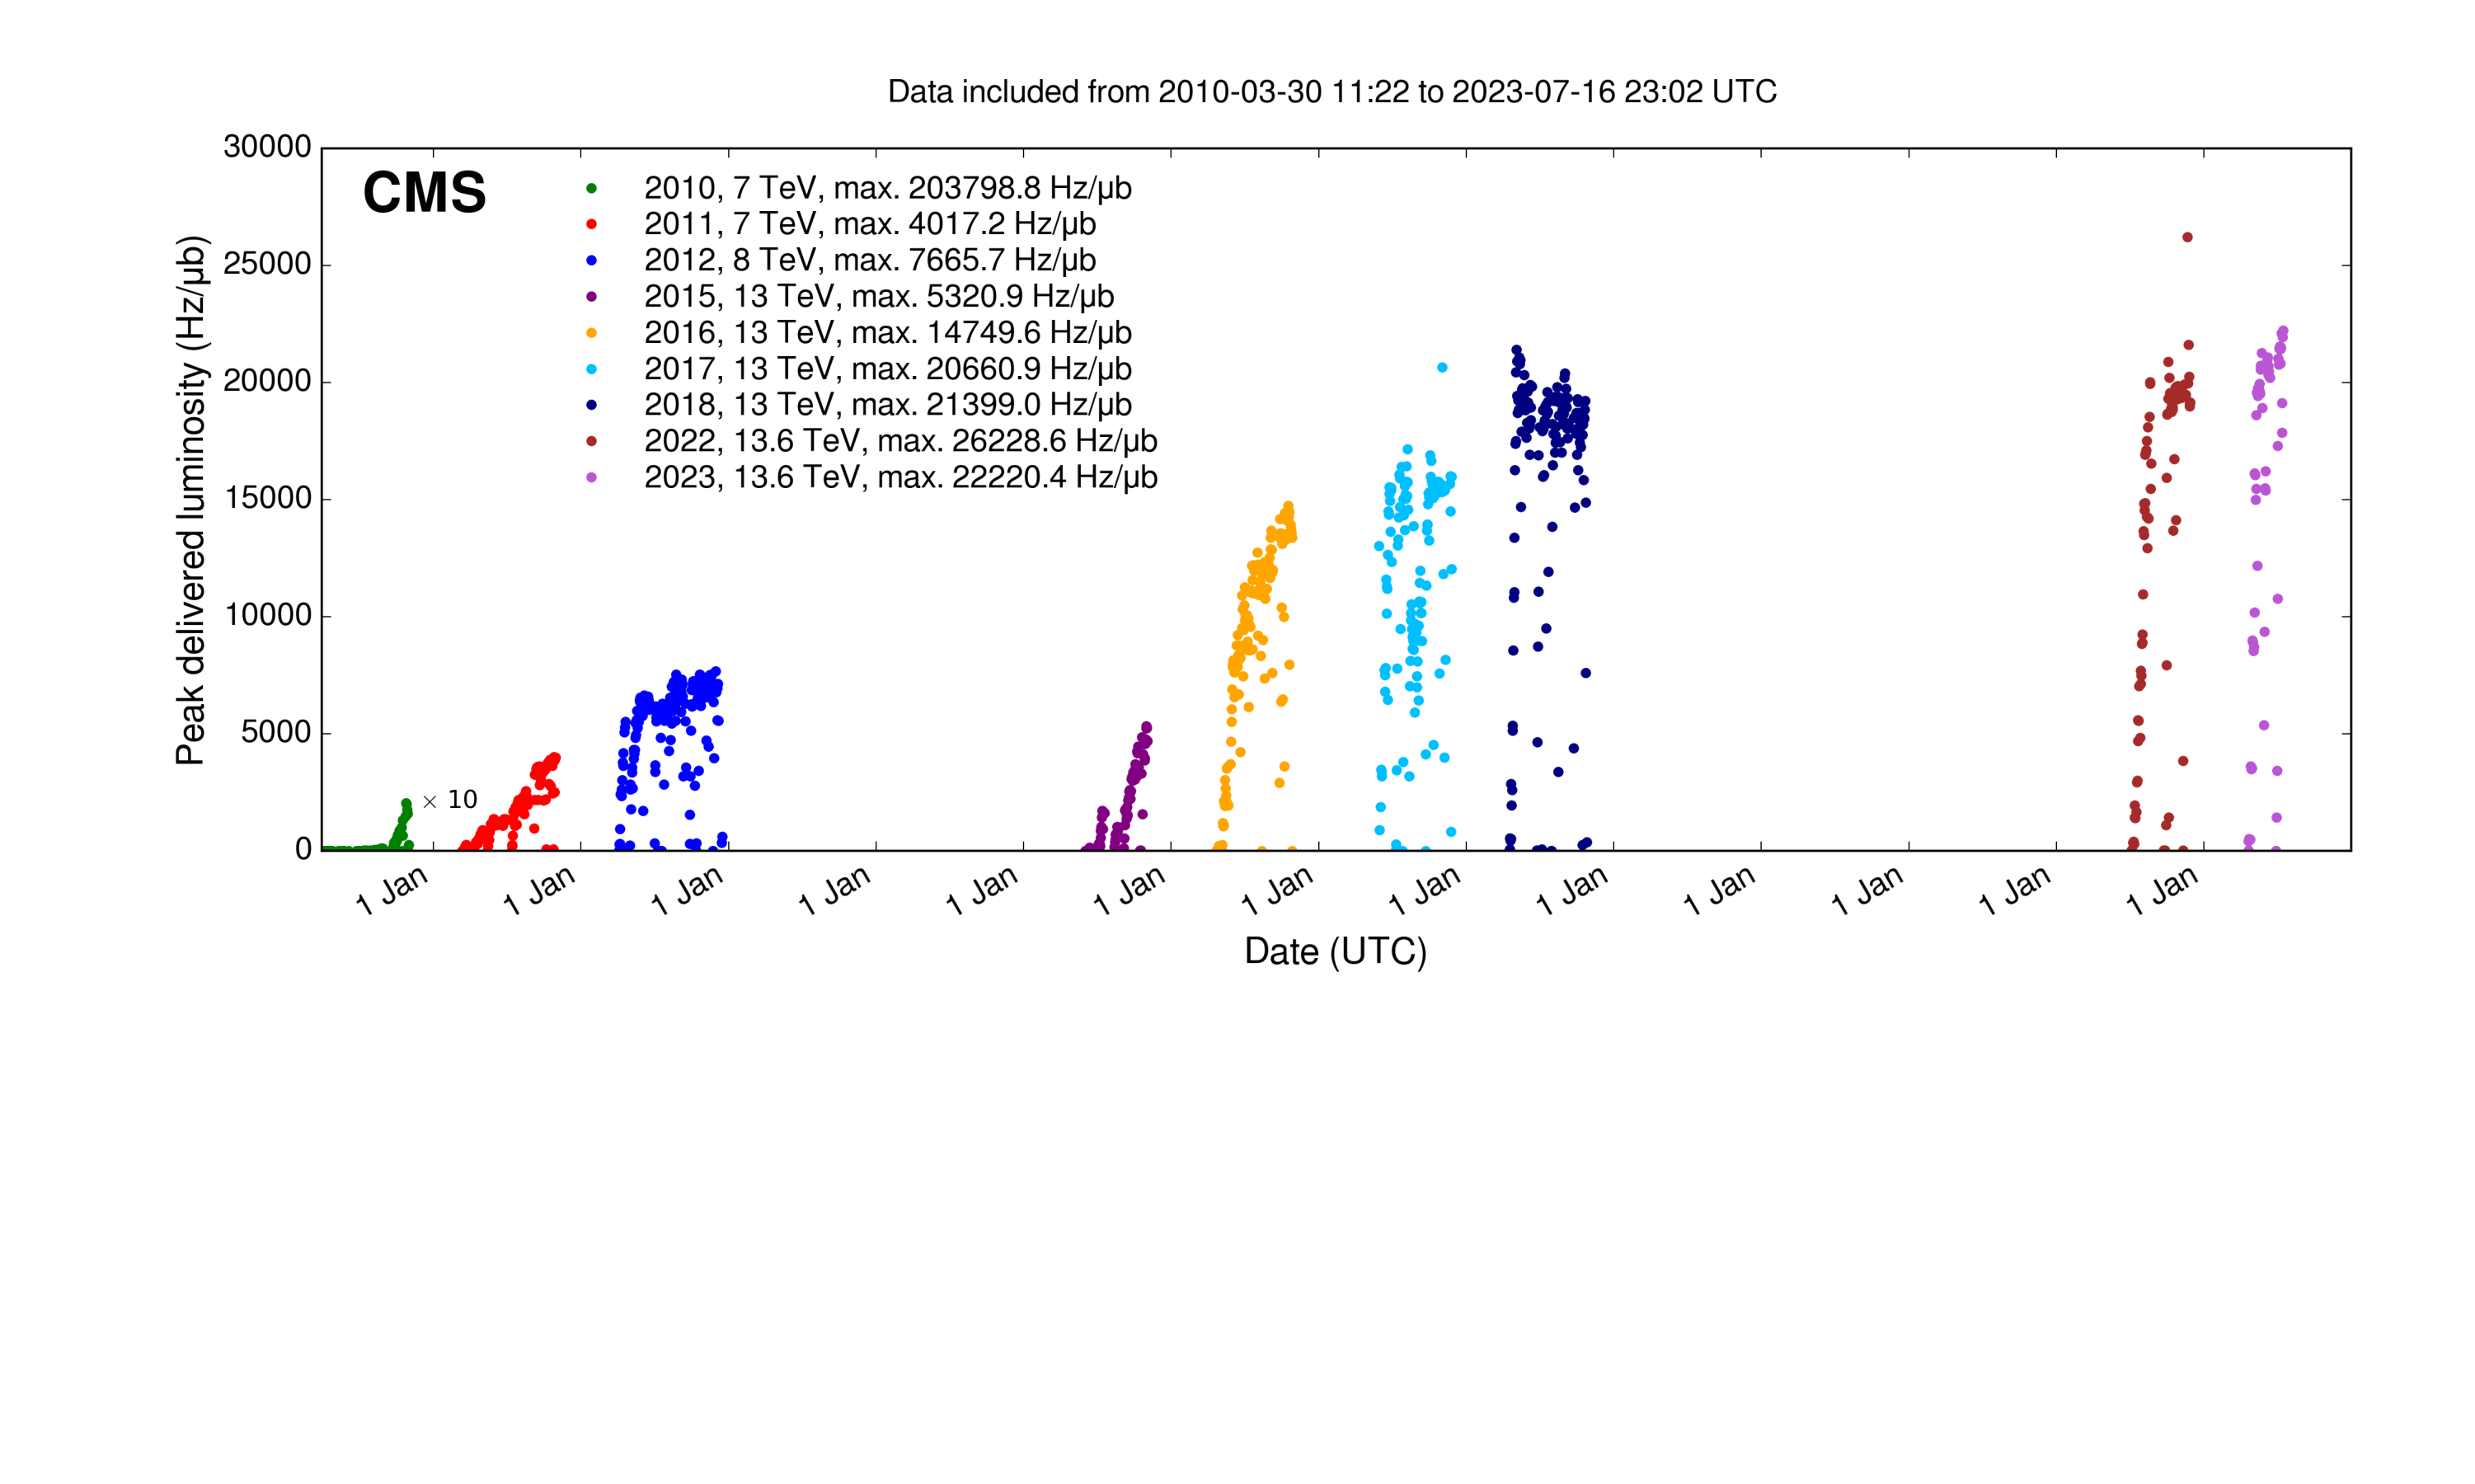
\includegraphics[width=\textwidth]{figures/Part2/Operation/peak_lumi_pp}
 \end{tabular}
 \caption{Peak luminosity versus day delivered to \ac{CMS} during stable beams and for proton-proton collisions, adapted from~\cite{twiki:lumi}.}
 \label{fig:peak}
 \end{center}
\end{figure}

Operations of the \ac{CMS} detector is coordinated by the \ac{CMS} Run Coordination, which is introduced in \autoref{sec:RC}. The \ac{CMS} control room is the commanding center of the \ac{CMS} operations, which is staffed 24$\times$7 during active data-taking period. Personnel who monitor and operate the \ac{CMS} detector from the control room are referred to as the ``central shift crew``, which is discussed further in \autoref{sec:ControlRoom}. In the In the context of detector operations, the principle contacts of the subsystems of the \ac{CMS} detector are known as the \ac{DOC} experts, or simply the \acp{DOC}. Core duties of one of the \acp{DOC}, the tracker \ac{DOC}, are described in \autoref{sec:DOC}.

\section{The CMS Run Coordination}
\label{sec:RC}

The \ac{CMS} detector is considered to be ``running'' when it is switched on and taking data. During this period, operations of various subsystems of the \ac{CMS} detector are controlled by the central shift crew. 

The Run Coordinators are responsible for the full scope of operations needed for the successful running of CMS. Strong cooperation with the Technical, Offline and Computing and Trigger Coordinators is required. Common areas of work occur in calibration and alignment, online database and trigger performance. Run Coordination is also responsible for monitoring aspects of data analysis coordination and the interaction with commissioning efforts in the Tracking, ECAL, HCAL, BRIL and Muon Detector Systems.

The Run Coordinators are responsible for the full scope of operations needed for the successful running of CMS. Strong cooperation with the Technical, Offline and Computing and Trigger Coordinators is required. Common areas of work occur in calibration and alignment, online database and trigger performance. Run Coordination is also responsible for monitoring aspects of data analysis coordination and the interaction with commissioning efforts in the Tracking, ECAL, HCAL, BRIL and Muon Detector Systems.

\section{Central Shift Crew}
\label{sec:ControlRoom}

The Run Coordinators are responsible for the full scope of operations needed for the successful running of CMS. Strong cooperation with the Technical, Offline and Computing and Trigger Coordinators is required. Common areas of work occur in calibration and alignment, online database and trigger performance. Run Coordination is also responsible for monitoring aspects of data analysis coordination and the interaction with commissioning efforts in the Tracking, ECAL, HCAL, BRIL and Muon Detector Systems.

The Run Coordinators are responsible for the full scope of operations needed for the successful running of CMS. Strong cooperation with the Technical, Offline and Computing and Trigger Coordinators is required. Common areas of work occur in calibration and alignment, online database and trigger performance. Run Coordination is also responsible for monitoring aspects of data analysis coordination and the interaction with commissioning efforts in the Tracking, ECAL, HCAL, BRIL and Muon Detector Systems.

\begin{figure}[tbh!]
 \begin{center}
 \begin{tabular}{c}
 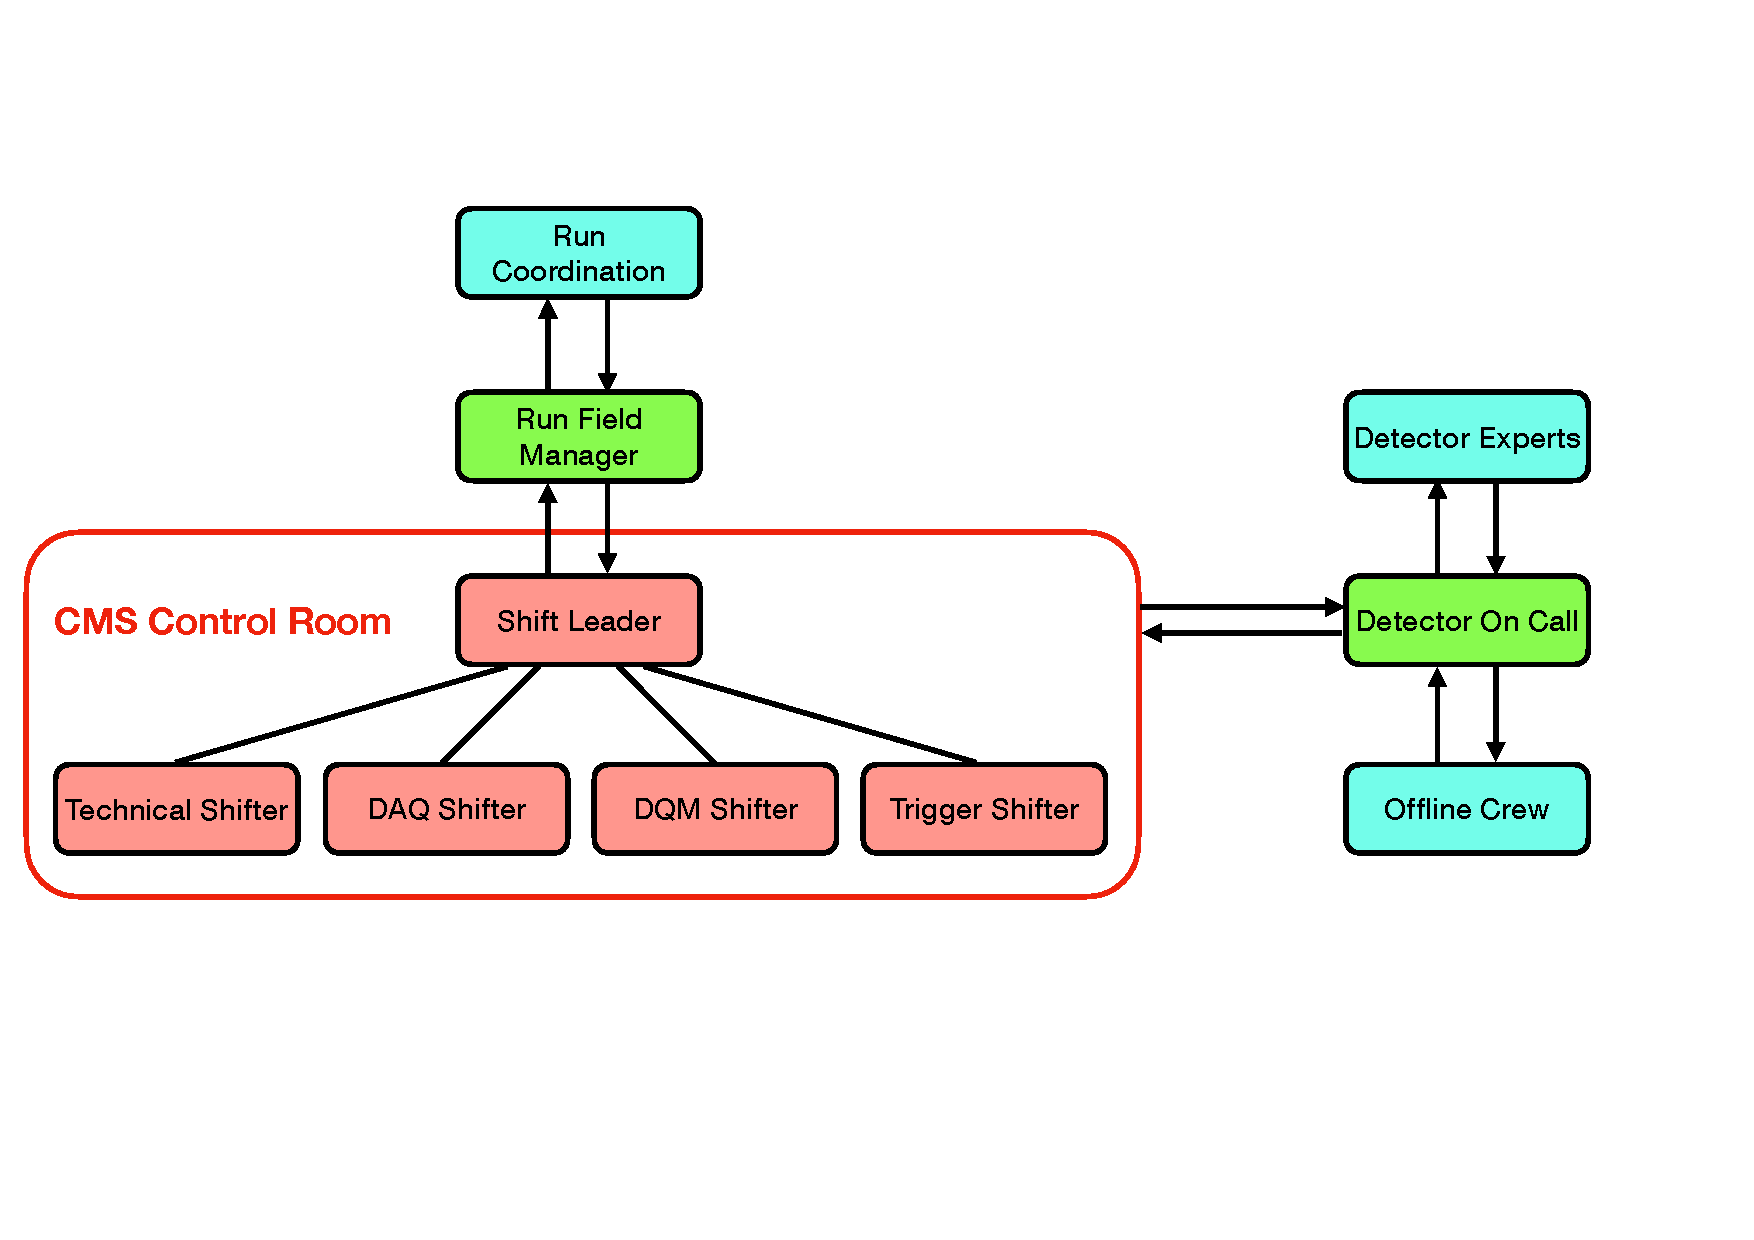
\includegraphics[width=0.9\textwidth]{figures/Part2/Operation/RC}
 \end{tabular}
 \caption{Main communication paths between various  the \ac{CMS} Run organization. The shift leader, technical, \ac{DAQ}, \ac{DQM}, and the trigger shifters are required to be present at the \ac{CMS} control room 24$\times$7. The \acp{RFM} and the \acp{DOC} are nominally present at the control room during the working hours. The Run Coordinators, subsystem expects, and offline shifters are not required to be at the control room although they often do.}
 \label{fig:RC}
 \end{center}
\end{figure}

The Run Coordinators are responsible for the full scope of operations needed for the successful running of CMS. Strong cooperation with the Technical, Offline and Computing and Trigger Coordinators is required. Common areas of work occur in calibration and alignment, online database and trigger performance. Run Coordination is also responsible for monitoring aspects of data analysis coordination and the interaction with commissioning efforts in the Tracking, ECAL, HCAL, BRIL and Muon Detector Systems.

\ac{DCS} \ac{DSS}

\section{Tracker Detector On-call Expert}
\label{sec:DOC}

One of the key goals of the \ac{CMS} tracker group is to ensure a stable and safe operation of the detector. This requires both well-trained operators as well as a modern \ac{DCS}. Built on top of the industrial product “WinCC”, the \ac{CMS} \ac{TCS}~\cite{Shah:2009zz,Karimeh:2020tzx} is designed to monitor the environmental conditions and safely operate the detector.

As part of the \ac{TCS} software, a \ac{FSM} toolkit is introduced. It is a powerful tool that assists operators in their daily job. It groups the power, cooling, dry gas and monitoring systems defined in the four \ac{TCS} projects in one hierarchical tree. The global state of the detector is continuously evaluated and made visible from the root Tracker FSM node giving critical information to the detector operator, as illustrated in Figure~\ref{fig:DCS}.

\begin{figure}[tbh!]
 \begin{center}
 \begin{tabular}{c}
 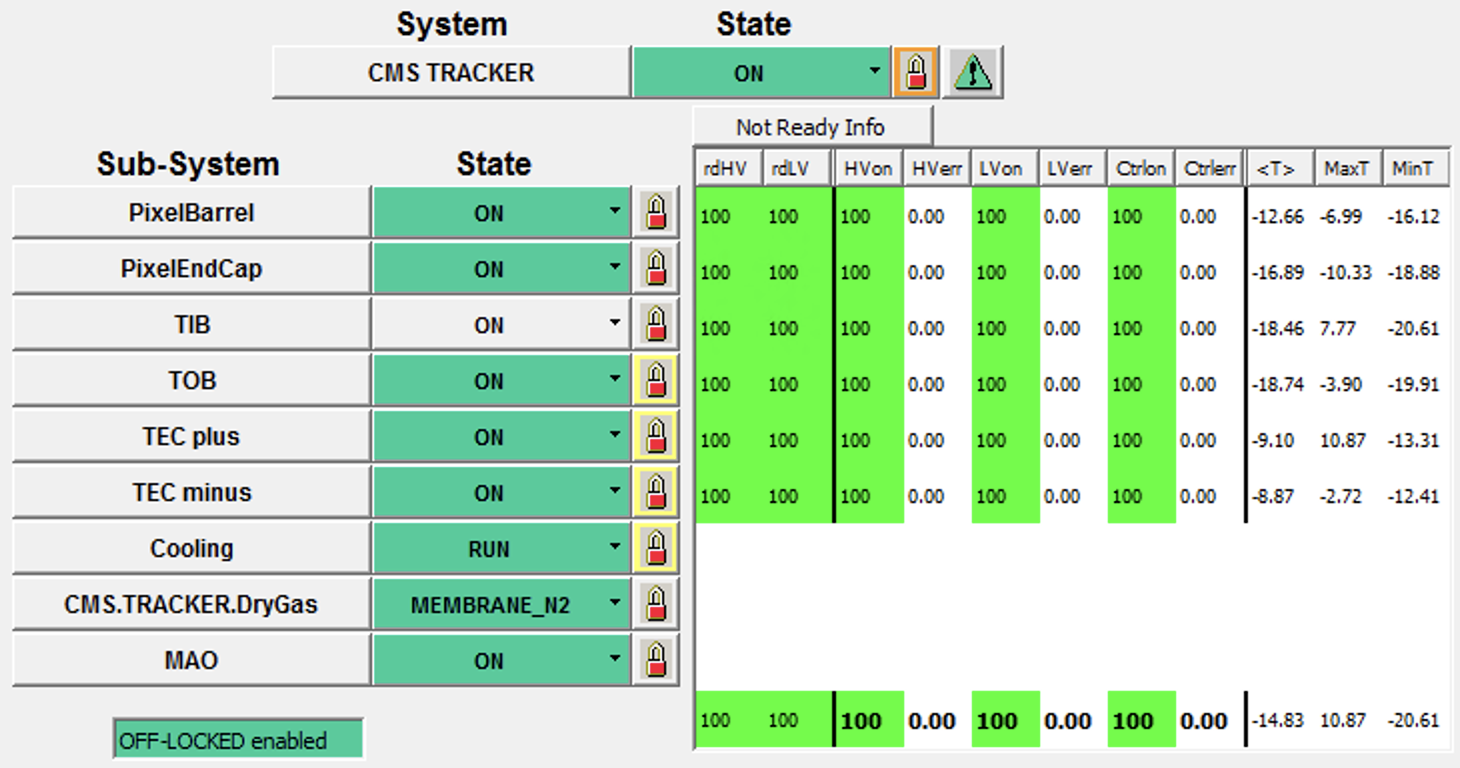
\includegraphics[width=0.8\textwidth]{figures/Part2/Operation/TrackerDCS}
 \end{tabular}
 \caption{Main panel of the tracker \ac{FSM}.}
 \label{fig:DCS}
 \end{center}
\end{figure}
\chapter{The Phase-2 Upgrade of the CMS Detector}
\label{chap:Upgrade}

Planned to start in 2029, the \ac{HL-LHC}~\cite{Apollinari:2017lan} will reach a peak instantaneous luminosity of up to $7.5\times10^{34}$cm$^{-2}$s$^{-1}$, as illustrated in Figure~\ref{fig:Lumi}. The increased luminosity will open up opportunities for ambitious physics programs including precision \ac{SM} measurements and searches for physics \ac{BSM}. To fully exploit the physics potential offered by the \ac{HL-LHC} datasets and overcome the challenging operational conditions, such as intense radiation and up to 200 \ac{PU} per event, the \ac{CMS} detector will undergo substantial upgrades during the \ac{LS} 3, known as the Phase-2 Upgrade~\cite{Contardo:2015bmq}.  

\begin{figure}[tbh!]
 \begin{center}
 \begin{tabular}{c}
 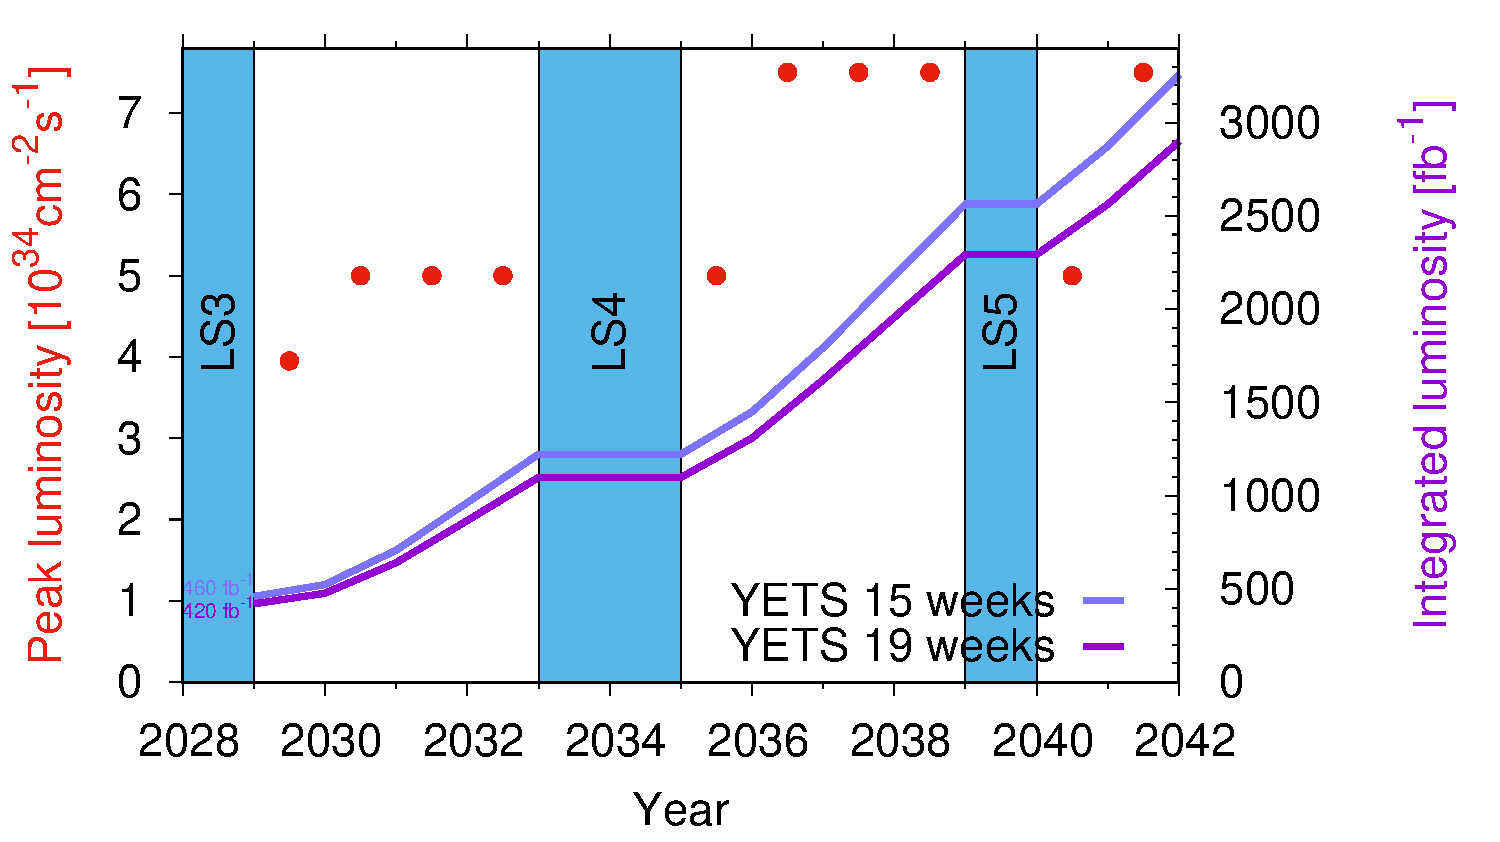
\includegraphics[width=0.8\textwidth]{figures/Part2/Upgrade/Lumi}
 \end{tabular}
 \caption{The peak and intergraded luminosity expected to be delivered by the \ac{HL-LHC}, taken from~\cite{LHC:plan} in November 2023. The left-hand $y$-axis shows the scale of the peak instantaneous luminosity, which is itself represented with red dots. The right-hand $y$-axis shows the scale of the intergraded luminosity. The two solid lines represent the intergraded luminosity under two \ac{YETS} scenarios.}
 \label{fig:Lumi}
 \end{center}
\end{figure}

An overview of the Phase-2 Upgrade is given in \autoref{sec:Overview}. Among various systems upgrades, the upgrade of the Outer Tracker is more relevant to this thesis, which is described in \autoref{sec:OT}. The Outer Tracker upgrade will enable tracking at the \ac{L1} trigger, which is discussed in \autoref{sec:Algo}. The tracking information can be combined with the calorimeter responses to build electron candidates at the \ac{L1} trigger, which is discussed in \autoref{sec:L1Ele}.

\section{Overview of the Upgrade}
\label{sec:Overview}

A new silicon tracker~\cite{CMS:2017lum} will replace the current tracker for the Phase-2. The Phase-2 tracker is divided into two subsystems: a pixel detector known as the Inner Tracker and the Outer Tracker composed of strip and macro-pixel sensors. Thanks to the extended coverage of the Inner Tracker, the Phase-2 Tracker will provide efficient tracking up to $|\eta|~<$ 4. The Phase-2 tracker is also much lighter with improved radiation hardness while enjoying a reduced material budget in the tracking volume. The granularity of the Phase-2 tracker will be increased by roughly a factor of 4, leading to a much better charged-particle $\pt$ resolution. More importantly, the Phase-2 Outer Tracker is specially designed to be capable of delivering data to the \ac{L1} trigger, which is further discussed in \autoref{sec:OT}.

The latency and event rate of the hardware-based \ac{L1} trigger will be increased (from 3.4 $\mu$s) to 12.5 $\mu$s and (from 100 kHz) 750 kHz, respectively, for the Phase-2~\cite{Zabi:2020gjd}. The increased latency leaves sufficient time for the track construction as well as correlating information from the tracker, calorimeters, and Muon system on \ac{L1} hardware. The addition of tracking information also enables the implementation of more sophisticated trigger algorithms at \ac{L1}, such as those based on the \ac{PF}~\cite{CMS:2017yfk} or \ac{PUPPI} algorithms~\cite{Bertolini:2014bba}.

The frontend electronics of the \ac{ECAL} Barrel Calorimeter will be replaced~\cite{ECAL:upgrade} to accommodate the latency and rate requirements of the Phase-2 \ac{L1} trigger, and to provide better timing resolution. The upgraded frontend electronics will enable the \ac{L1} trigger to exploit the information from single crystals as opposed to the trigger primitive of $5\times5$ crystals provided by the current system. The more granular trigger primitives will improve the precision of identifications and isolations of calorimeter objects and the matching between tracks and electromagnetic showers at \ac{L1}. 

The \ac{ECAL} and \ac{HCAL} Endcap Calorimeters will be replaced by a new endcap calorimeter known as the \ac{HGCAL}~\cite{CMS:2017jpq}. The \ac{HGCAL} is a sampling calorimeter consisting of both electromagnetic
and hadronic sections, which are designed to withstand the extreme radiation level at the \ac{HL-LHC}. It provides an excellent timing resolution and incorporates the concept of three-dimensional shower measurements from experiments at the \ac{ILC}~\cite{CALICE:2008kht}. Like both of its predecessors, the \ac{HGCAL} is designed to contribute to the \ac{L1} trigger.

A brand new subsystem known as the \ac{MTD}~\cite{Butler:2019rpu} will be added to the \ac{CMS} Phase-2 lineup. The \ac{MTD} covers both barrel and endcap regions and it enables the measurements of the production timing of the \acp{MIP}. This addition enables the four-dimensional reconstruction of the interacting vertices, which represents a completely new capability added to the \ac{CMS} detector. The timing information associated with the reconstructed vertices will provide a much-needed handle to cope with the high \ac{PU} conditions at the \ac{HL-LHC}.

As explained in \autoref{sec:MuonSys}, the \ac{CSC} in the endcap region will be complemented by a new subsystem \ac{GEM}, which is expected to be fully operational by \ac{LS} 3. Similar to the \ac{ECAL} Barrel, the electronics of the Muon system will also be upgraded to meet the \ac{L1} trigger requirements~\cite{Hebbeker:2017bix}.

Upgrades of the \ac{HLT} and \ac{BRIL} system are also planned and are documented in detail in Ref.~\cite{HLT:Upgrade} and~\cite{Beam:Upgrade}, respectively. 

\section{The Outer Tracker Upgrade}
\label{sec:OT}

The performance of the current \ac{CMS} Tracker will be significantly degraded if it continues to take data beyond the designed radiation exposure (500 fb$^{-1}$) in the \ac{HL-LHC} era. Therefore, it must be completely replaced by a new tracker by the end of Run-3, which is envisioned to be able to withstand radiation damage up to 3000 fb$^{-1}$. 

The design of the Phase-2 Outer tracker is largely driven by the task of providing tracking information to the \ac{L1} trigger. The feasibility of a track trigger at \ac{L1} is significantly challenged by the sheer data volume generated by the \ac{HL-LHC} at a frequency of 40 MHz accompanied by up to 200 \ac{PU}. A novel tracker module design, known as the ``$\pt$ module''~\cite{Foudas:2005xf} is used to reduce the data volume effectively while keeping interesting events for physics analyses. Under this design, the Outer tracker will be composed of over three thousand $\pt$ modules, and each consists of two closely spaced silicon sensors that are parallel to each other. Through correlating hits from the two parallel sensors, the $\pt$ modules are capable of providing $\pt$ discrimination, thus reducing the data volume at the front end. Correlated pairs of hits are referred to as ``stubs'', which serve as the trigger primitive to the \ac{L1} trigger. The stub mechanism is illustrated in Figure~\ref{fig:Stub}. With the current design, only hits over the threshold of 2 GeV will be read out, which corresponds to a data reduction rate of up to 100.

\begin{figure}[tbh!]
 \begin{center}
 \begin{tabular}{cc}
  \centering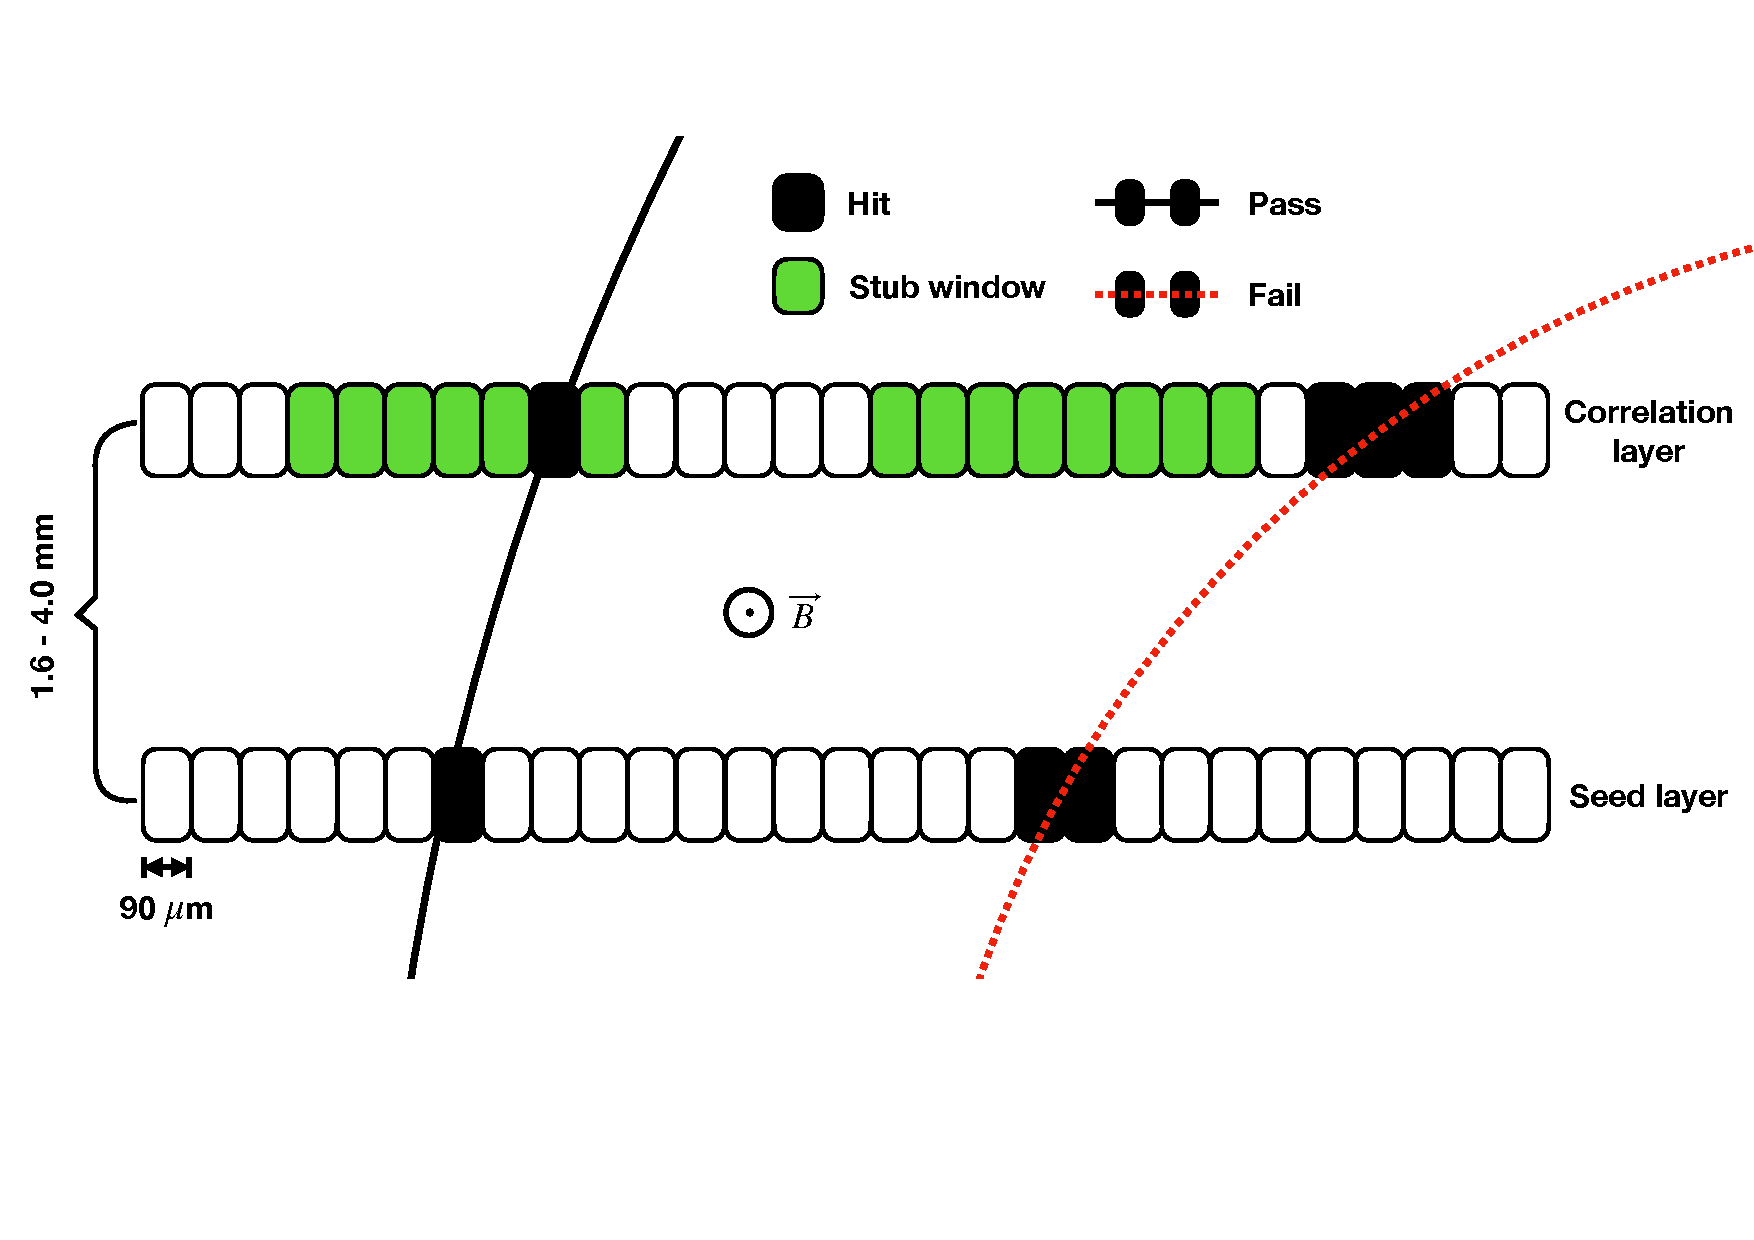
\includegraphics[width=0.9\linewidth]{figures/Part2/Upgrade/Stub}
 \end{tabular}
 \caption{Illustration of the stub mechanism in a cross-sectional view of a $\pt$ module (2S) in the magnetic field. Charged particles with a $\pt$ higher than 2 GeV are represented with the black solid curve while the red dashed curve represents charge particles with lower $\pt$. The magnetic field will cause low $\pt$ charged particles to bend with a smaller radius of curvature, and thus fail the pre-determined stub window corresponding to a $\pt$ threshold of 2 GeV.}
 \label{fig:Stub}
 \end{center}
\end{figure}

The Phase-2 Outer Tracker consists of six cylindrical barrel layers (L1-L6) and five disks (D1-D5) on each side of the endcap, as illustrated in \ref{fig:TrackerGeo}. The layers and disks of the Outer Tracker are composed of two types of $\pt$ modules, known as the ``Pixel-Strip (PS)'' modules and ``Strip-Strip (2S)'' modules. Sketches of the PS and 2S modules are shown in Figure~\ref{fig:Modules}. The PS modules occupy the first three barrel layers as well as regions of the disks that are closer to the beam line. The remaining regions of the disks as well as the last three barrel layers are occupied by the 2S modules. The Outer Tracker layout shown in figure~\ref{fig:TrackerGeo} is known as the so-called ``tilted geometry'' where the PS modules in the barrel layers are positioned with various titled angles to increase the stub efficiency.

\begin{figure}[tbh!]
 \begin{center}
 \begin{tabular}{c}
  \centering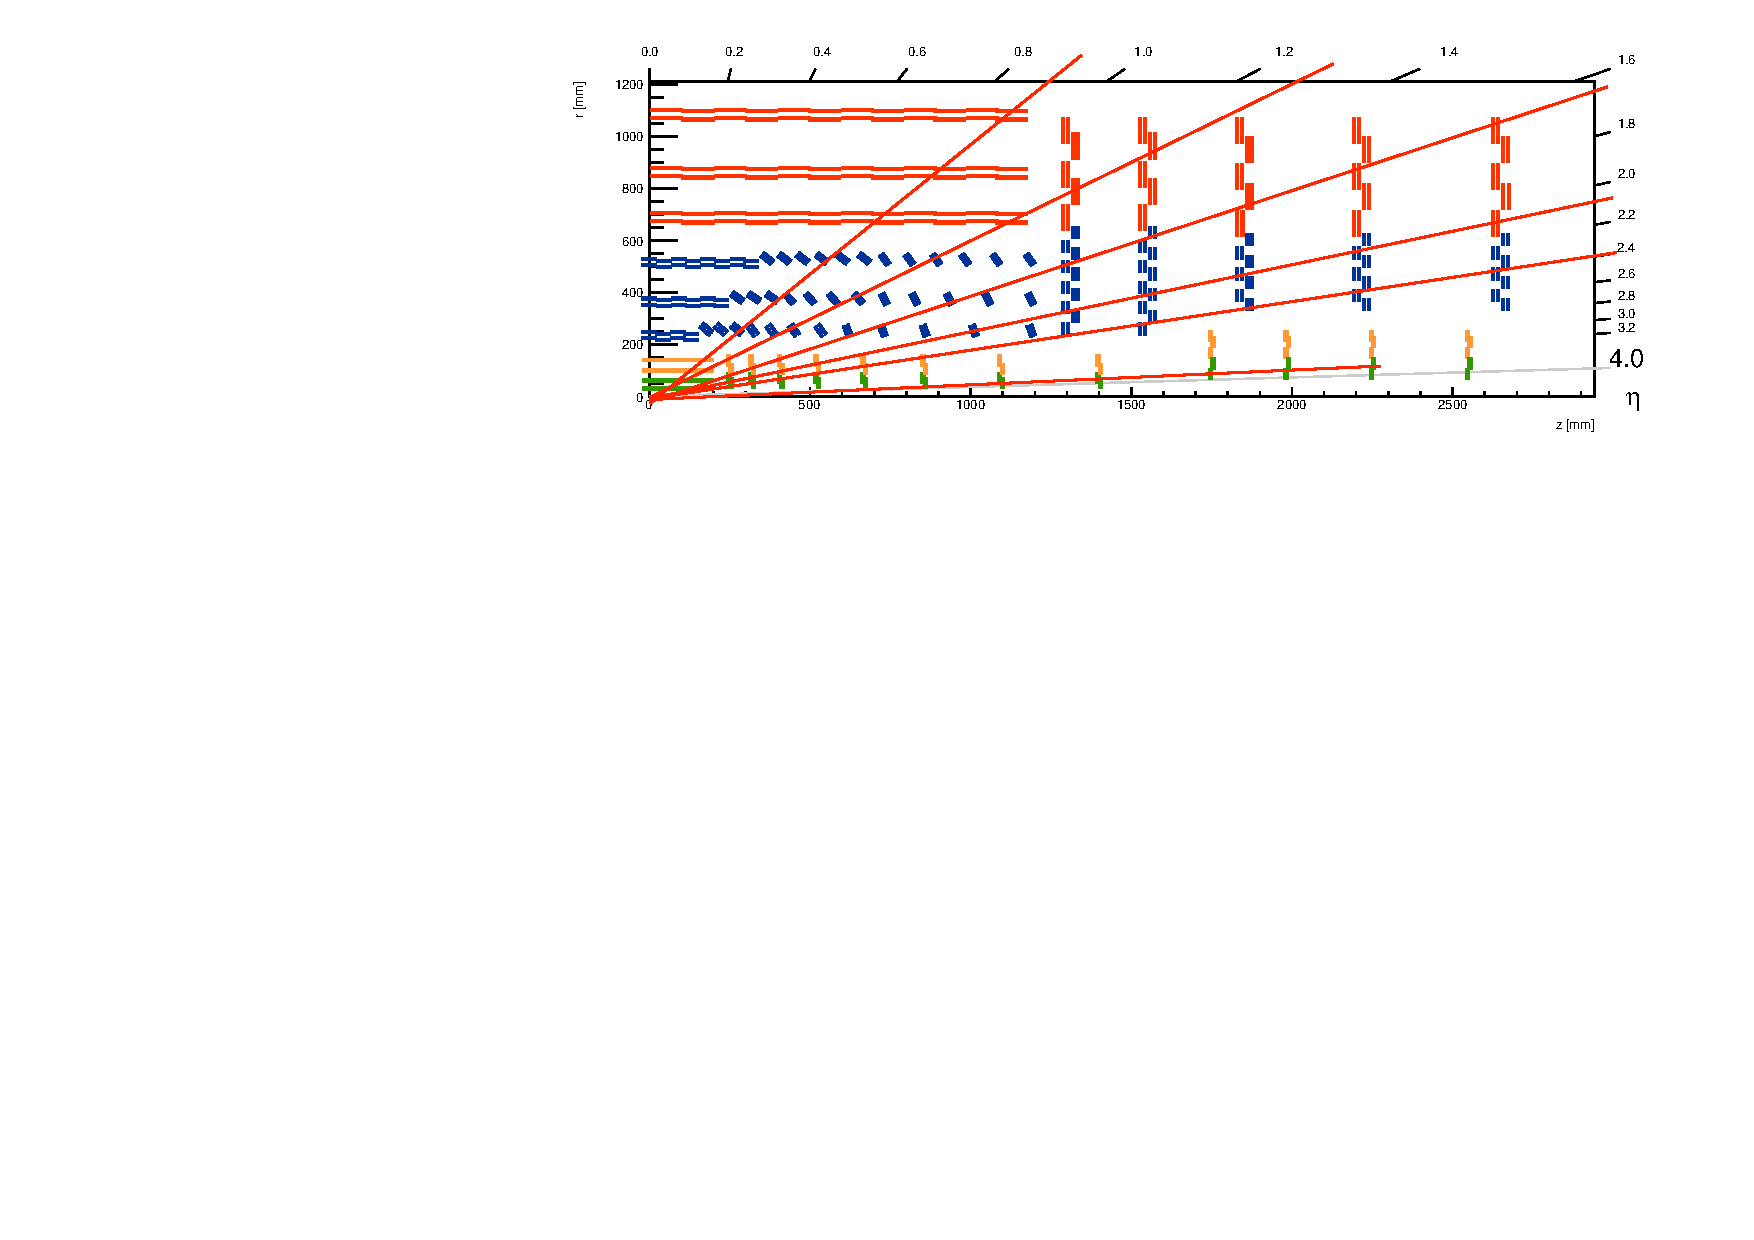
\includegraphics[width=0.9\linewidth]{figures/Part2/Upgrade/TrackerGeo}
 \end{tabular}
 \caption{Layout of one quadrant of the Phase-2 \ac{CMS} tracker in the $r-z$ plane, generated by the \ac{CMSSW}~\cite{cmssw}. The PS modules of the Outer Tracker are represented with blue lines while the 2S modules are represented with red lines. The radial region below 200 mm is occupied by the Inner Tracker, whose modules are represented with orange and green lines. The Inner Tracker does not contribute to the \ac{L1} trigger.}
 \label{fig:TrackerGeo}
 \end{center}
\end{figure}

\begin{figure}[tbh!]
 \begin{center}
 \begin{tabular}{c}
  \centering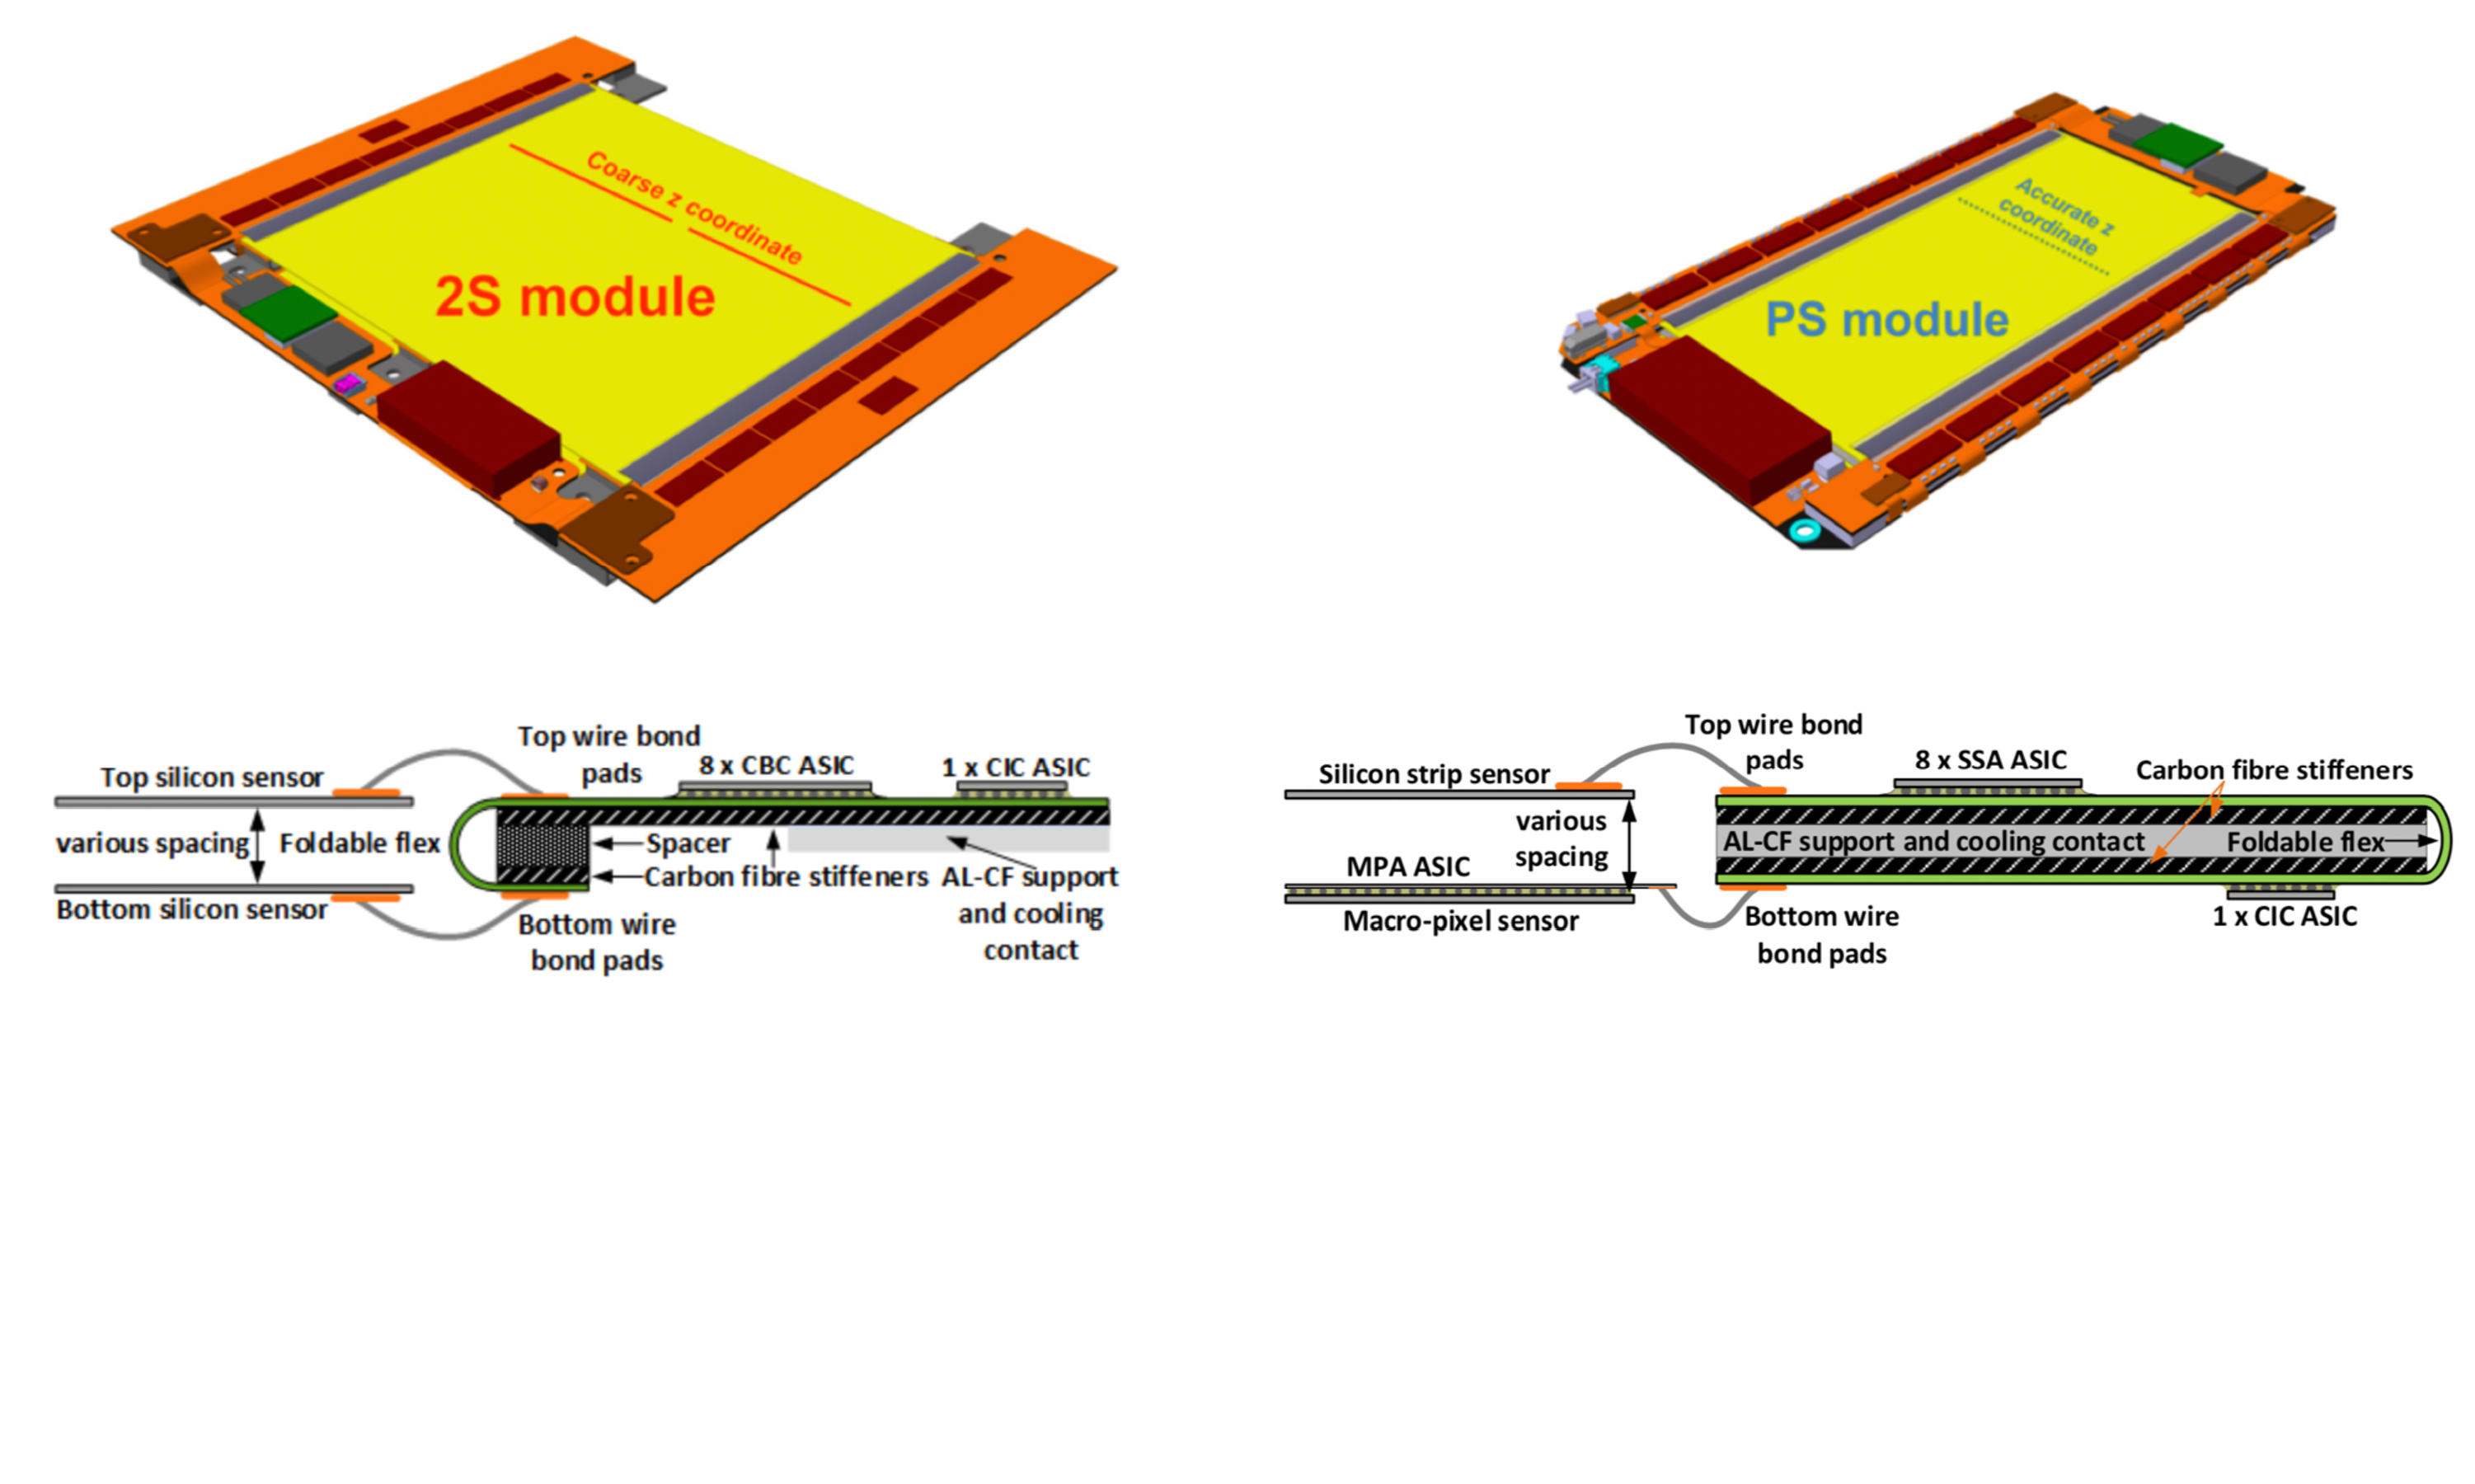
\includegraphics[width=0.95\linewidth]{figures/Part2/Upgrade/Modules}
 \end{tabular}
 \caption{Illustrations of the 2S module (left) and PS module (right), adapted from~\cite{CMS:2017lum}. Shown are views of the assembled modules (top) and sketches of the connection between frontend hybrids and silicon sensors (bottom).}
 \label{fig:Modules}
 \end{center}
\end{figure}

The 2S module consists of two 90 cm$^{2}$ strip sensors separated by a few millimeters using a \ac{Al-CF} spacer. Each strip sensor consists of over two thousand strips arranged in two rows. Each strip is 5 cm long with a pitch of 90 $\mu$m. The two sensors are connected to hybrid circuits known as the frontend hybrid and service hybrid. The frontend hybrid consists of eight \ac{CBC}~\cite{Raymond:2012zz}, which is responsible for readout. The service hybrid is mainly responsible for powering.

The PS module is about half the size of the 2S module in its active area. It has one strip sensor on the top and one macro-pixel sensor on the bottom, which provides very precise measurements of $z$-coordinates. Similar to the 2S module, the strip sensor of the PS module consists of roughly two thousand strips. Each strip is about 2.4 cm long with a pitch of 100 $\mu$m. The macro-pixel sensor contains 960 $\times$ 32 macro-pixels with a length and pitch of 1.5 cm and 100 $\mu$m, respectively. The two sensors are connected to hybrid circuits that are responsible for readout~\cite{Ceresa:2016mqm} and powering.

\section{Leve-1 Track Finder}
\label{sec:Algo}

The task for track finding algorithms at \ac{L1} can be broken down into two main parts: i) performing pattern recognition to identify and correlate all possible stubs that belong to the same charged particle trajectory and ii) obtaining the parameters of the trajectory by fitting the reconstructed tracks. A latency of roughly 4 $\mu$s is allocated to track finding algorithms, which becomes one of the critical constraints in algorithm development. Multiple approaches~\cite{CMS:2017lum} have demonstrated the feasibility of delivering tracking information within the allowed latency and a so-called ``hybrid'' approach~\cite{Zabi:2020gjd} is adopted by \ac{CMS} as the way forward.

To meet the latency requirement and increase redundancy, the hybrid approach is parallelized both in space and in time. The Outer Tracker is partitioned into nine $\phi$ sectors and stubs in each sector are processed in parallel with a time-multiplexing factor of up to 18. The main stages of the hybrid approach are similar to the offline \ac{CTF} algorithm described in \autoref{sec:Track}, including seeding, pattern recognition, and parameter fitting, as illustrated in Figure~\ref{fig:algorithm}. The main difference is that the parameter fitting is disentangled from the pattern recognition in the hybrid approach while these two stages are intergraded in the \ac{CTF} algorithm.

\begin{figure}[tbh!]
 \begin{center}
 \begin{tabular}{cc}
  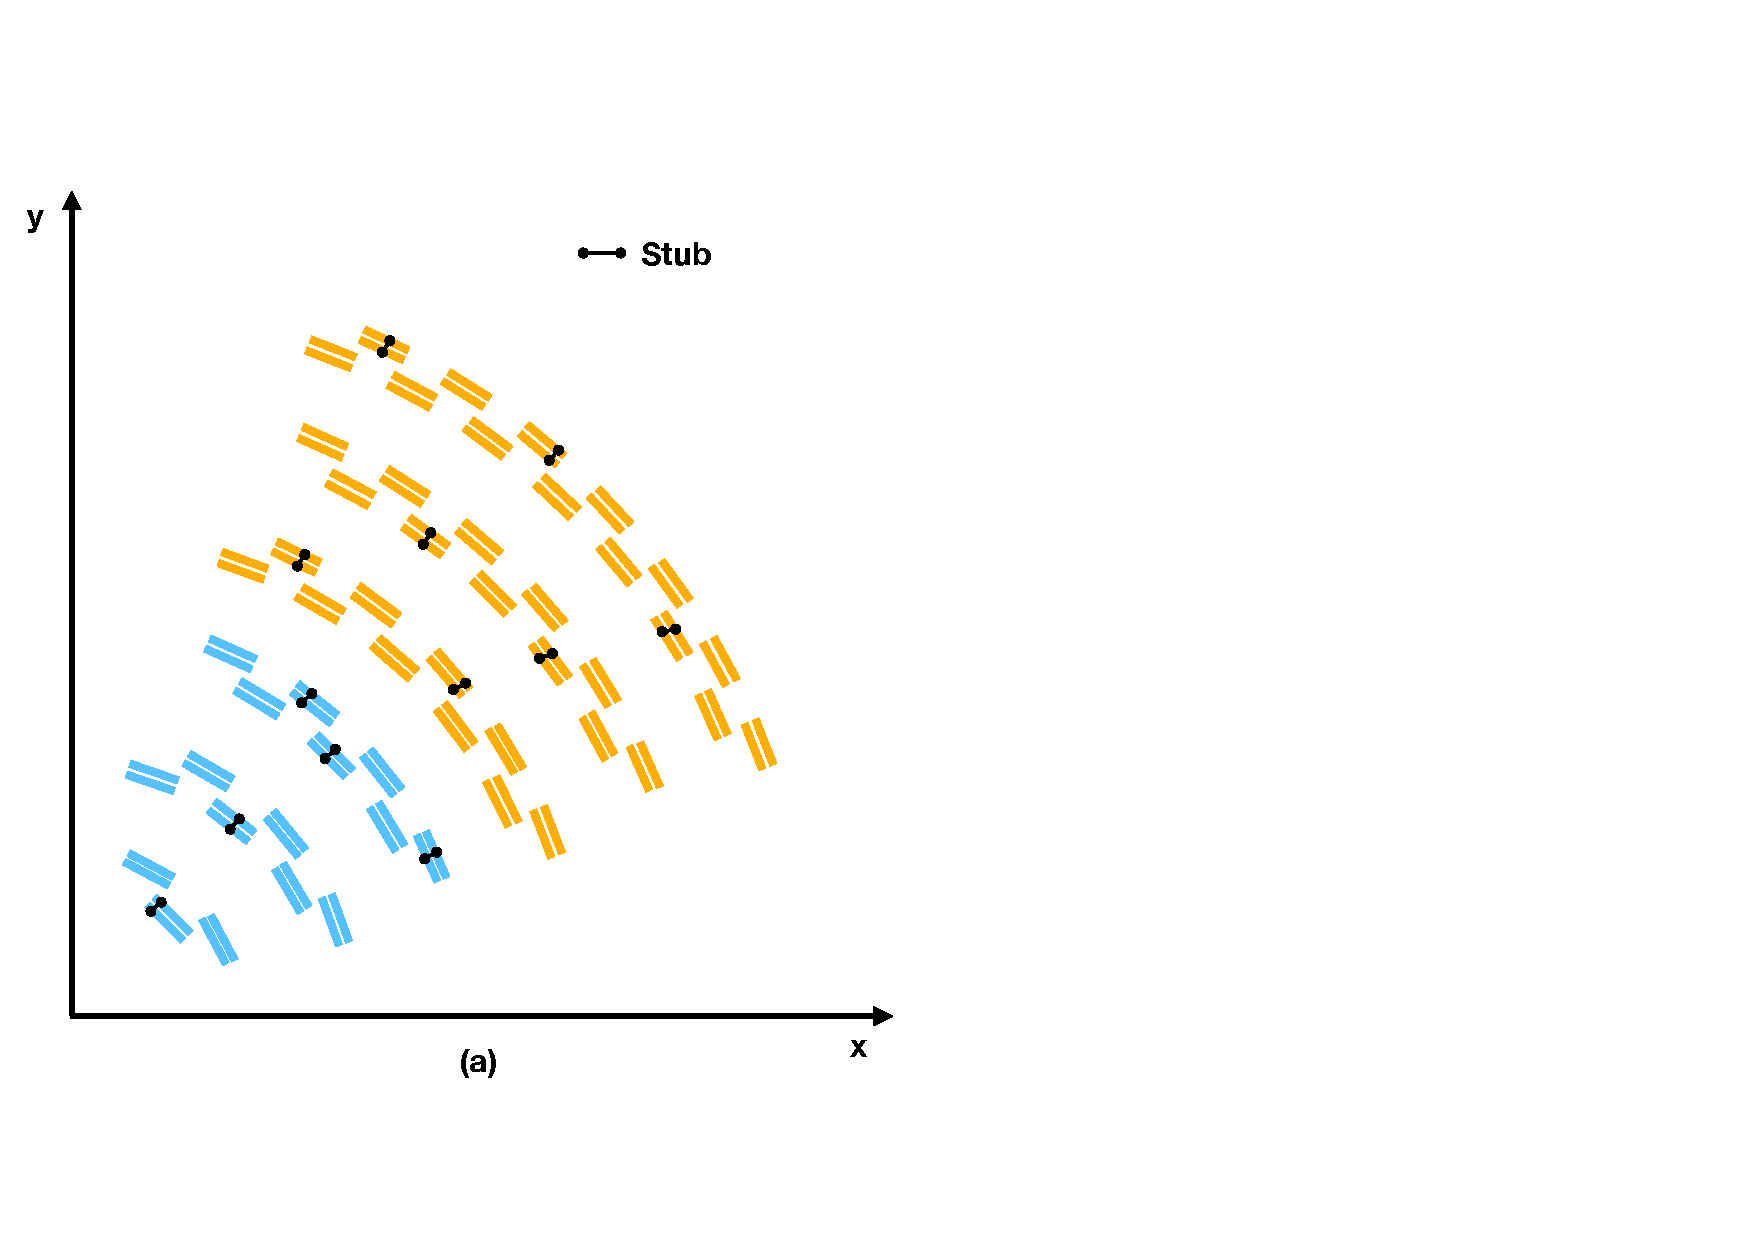
\includegraphics[width=.45\linewidth]{figures/Part2/Upgrade/tracklet1} &
  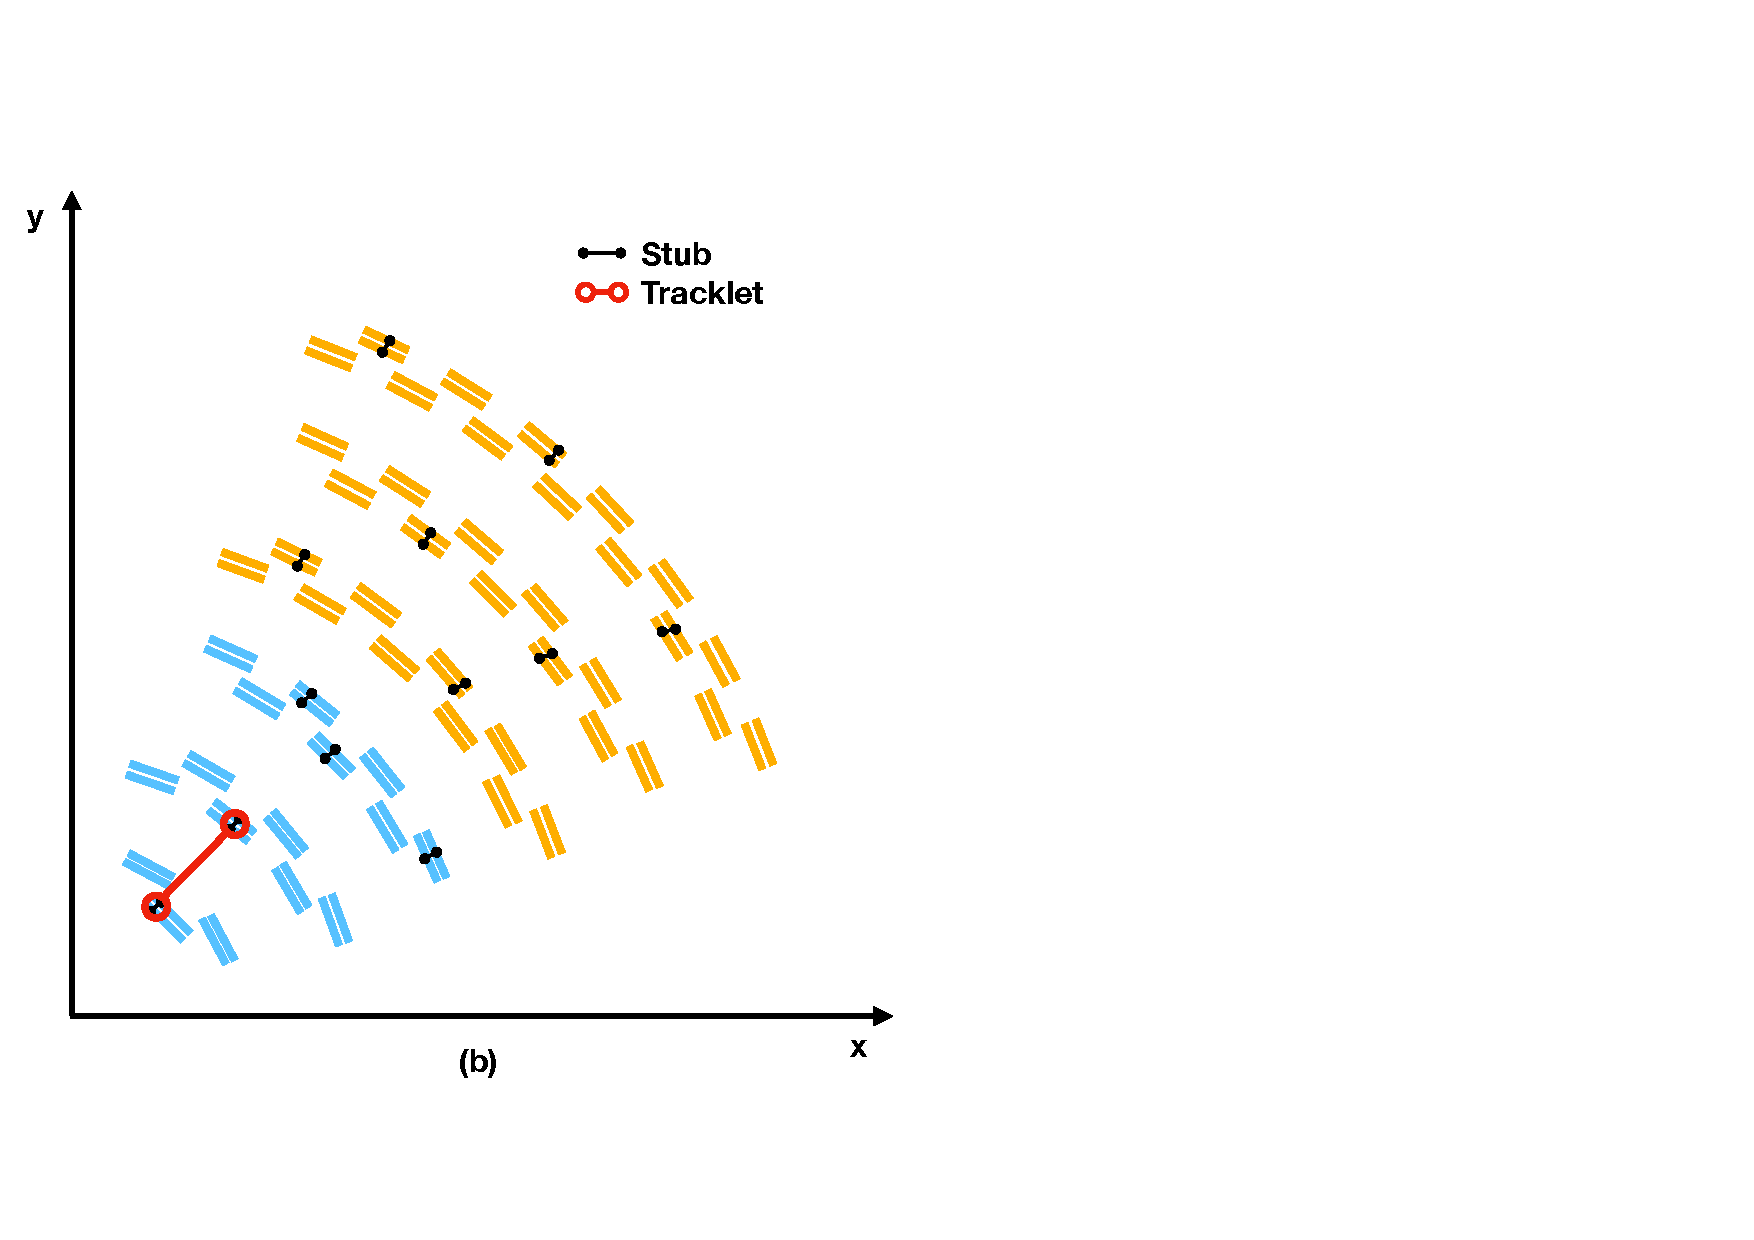
\includegraphics[width=.45\linewidth]{figures/Part2/Upgrade/tracklet2} \\
  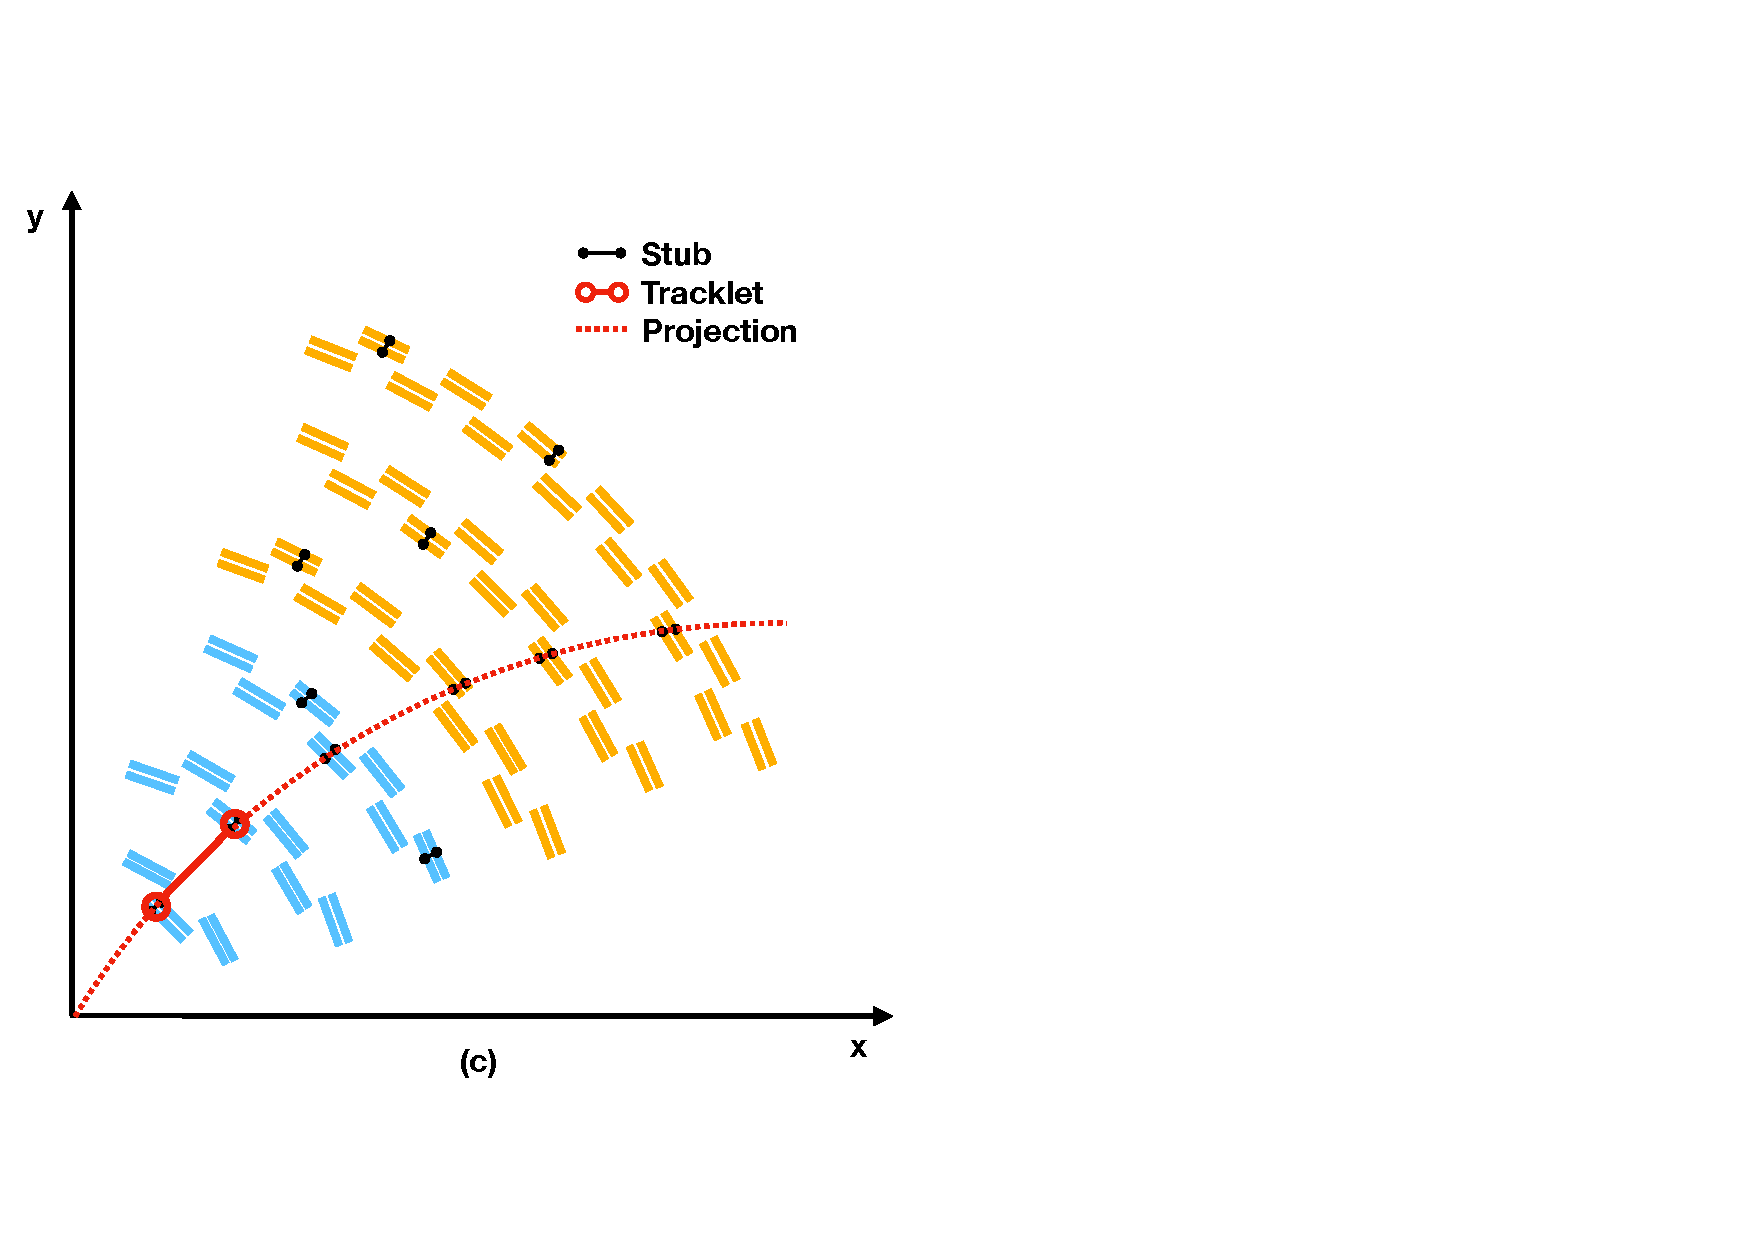
\includegraphics[width=.45\linewidth]{figures/Part2/Upgrade/tracklet3} &
  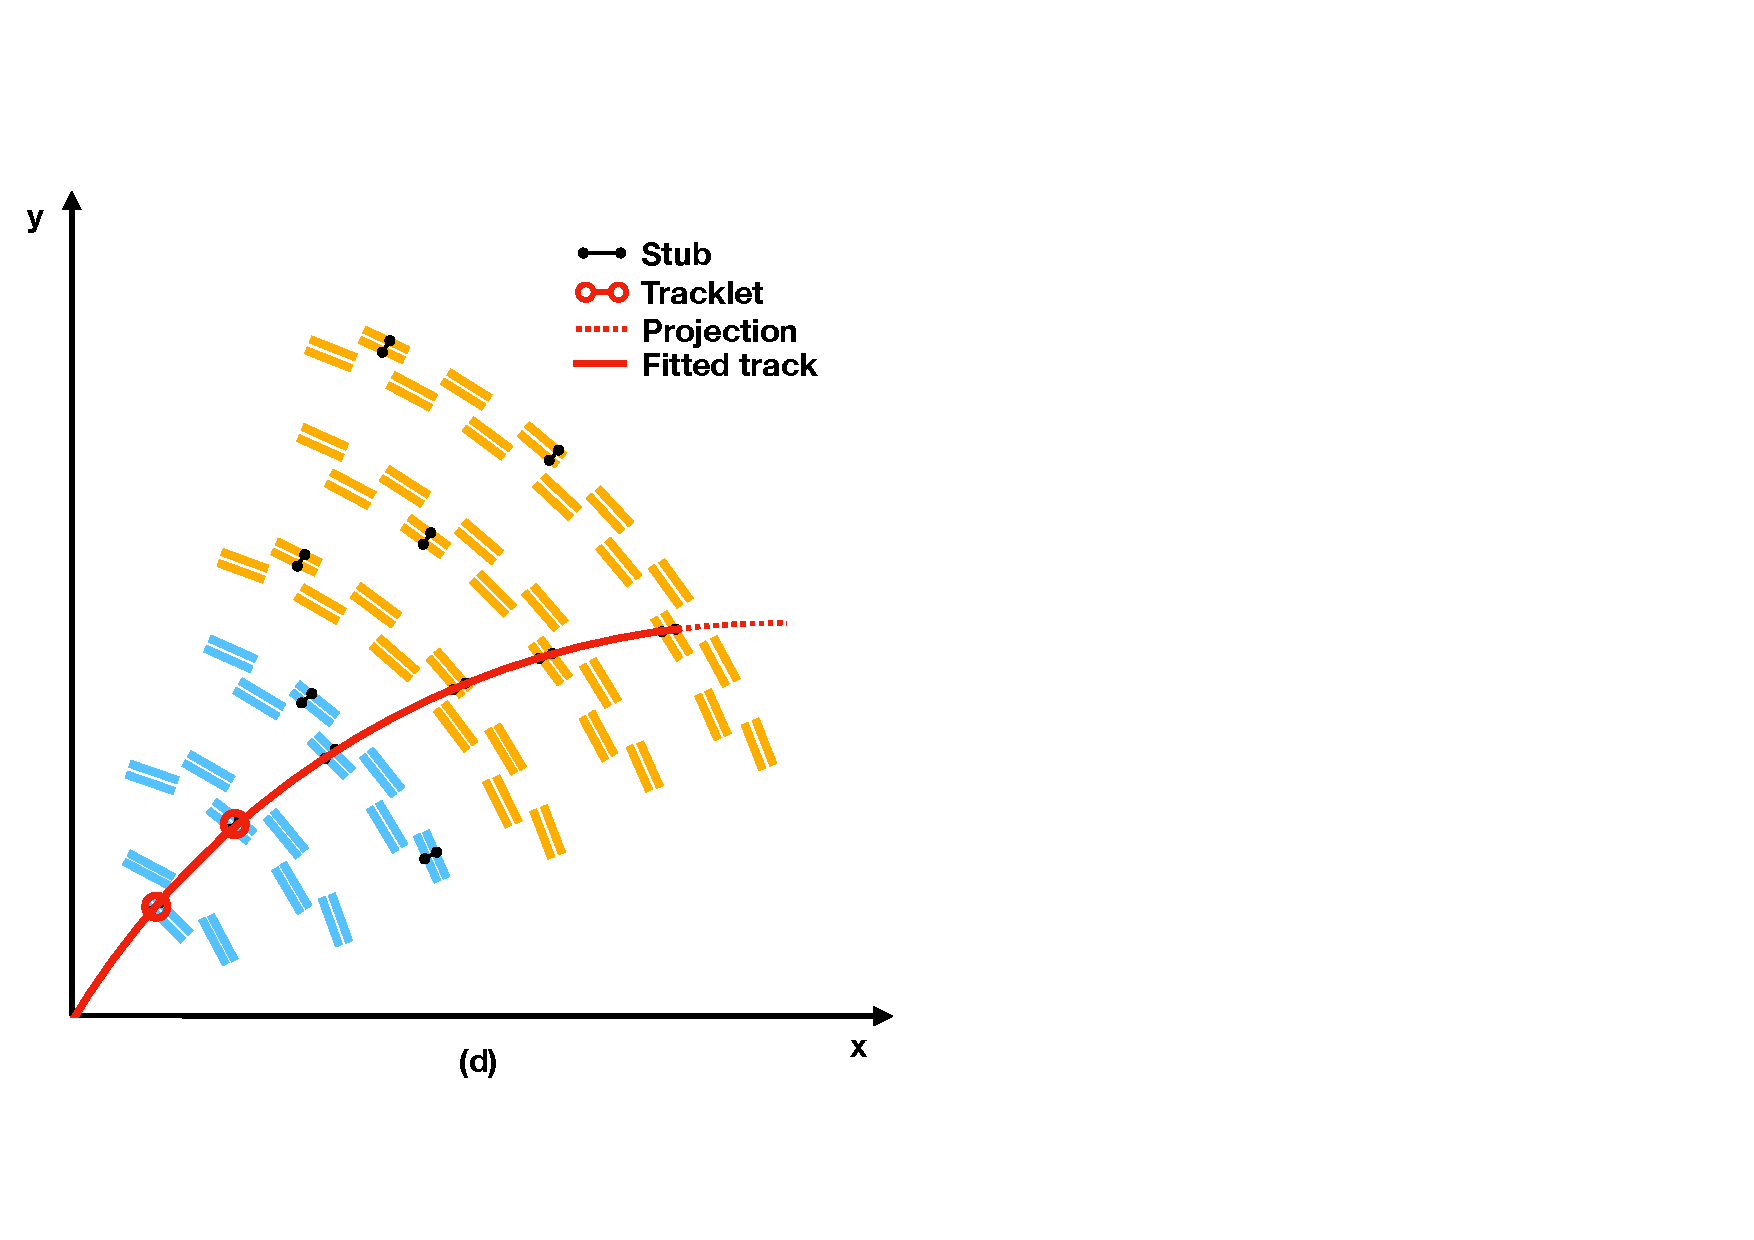
\includegraphics[width=.45\linewidth]{figures/Part2/Upgrade/tracklet4} \\
 \end{tabular}
 \caption{Illustration of different stages of the hybrid approach: (a) constructing stubs, (b) forming tracklet by correlating two stubs and the beam spot (origin), (c) projecting to other layers and finding matches, and (d) fitting track parameters using a \ac{KF}.}
 \label{fig:algorithm}
 \end{center}
\end{figure}

The initial stage of the hybrid approach involves correlating two stubs from two different Outer Tracker layers or disks under the assumption that trajectories of the charged particles originate from the beam spot. The correlated pair of stubs is referred to as the ``tracklet'' which is later used as a seed for the pattern recognition. The tracklet also comes with coarse parameter estimates which will be updated in the fitting stage. Seven combinations of layers/disks are attempted in parallel for seeding: L1+L2, L3+L4, L5+L6, D1+D2, D3+D4, L1+D1, and L2+D1. 

Based on its initial parameters, the tracklet is then extrapolated inward and outward to all possible layers or disks in parallel to look for stubs that belong to the same trajectory. A match is declared if a stub is found within a predetermined window around the projection in a layer or disk. At least two matches are needed in order to proceed to the following stage. 

Duplicates of the same track are produced as a result of the highly parallelized approach. Duplicated tracks are typically produced by two adjacent $\phi$ sectors when a charged particle is located near the sector boundary. Alternatively, they can be tracks that belong to the same sector but are seeded by different layer/disk combinations. To remove duplicates tracks that share common stubs will be merged before the parameter fitting. 

The fitting stage is done by a \ac{KF} module that possesses the initial track parameters and adds stubs iteratively to update the track parameters. Each time a new stub is added, the consistency between the existing track parameters and the new stub will be checked which provides input to the parameter update. All potential combinations of stubs are attempted by the \ac{KF}, and the final residual of each combination is calculated and compared. The stub combination with the best residual is finally chosen as the \ac{KF} output. 

Tracks coming out of the fitting stage are considered to be the final product since all the track parameters are final. Similar to the offline track finder discussed in \ref{sec:Track}, fake tracks can still be reconstructed by the \ac{L1} track finder due to a variety of constraints and limitations of the algorithm. An additional module, referred to as the ``track quality'' is added to help distinguish, in a \ac{MVA} approach, between genuine tracks that can be associated with charged particles and fake tracks. A score between 0 and 1 is calculated for each track by combining multiple variables, such as the residuals produced by the \ac{KF}, into a \ac{BDT}. The score assigned to each track roughly translates to the probability of this track being genuine.

The hybrid track-finding algorithm has demonstrated a robust performance in software simulation, as shown in Figure~\ref{fig:trackingperformance}. The baseline version of this algorithm requires stubs from at least four unique layers and constrains the origin of the trajectories to the beam spot. An ``extended'' version of the algorithm is also in development, in which the beam spot constraint is relaxed. The extended tracking is especially useful in scenarios where tracks originate with a small displacement in the transverse plane, such as displaced electrons as a result of bremsstrahlung in the Inner Tracker. It has been shown that sizable improvement in electron tracking efficiency can be achieved by the extended tracking algorithm, as shown in Figure~\ref{fig:electronperformance}.

 \begin{figure}[tbh!]
 \begin{center}
 \begin{tabular}{cc}
  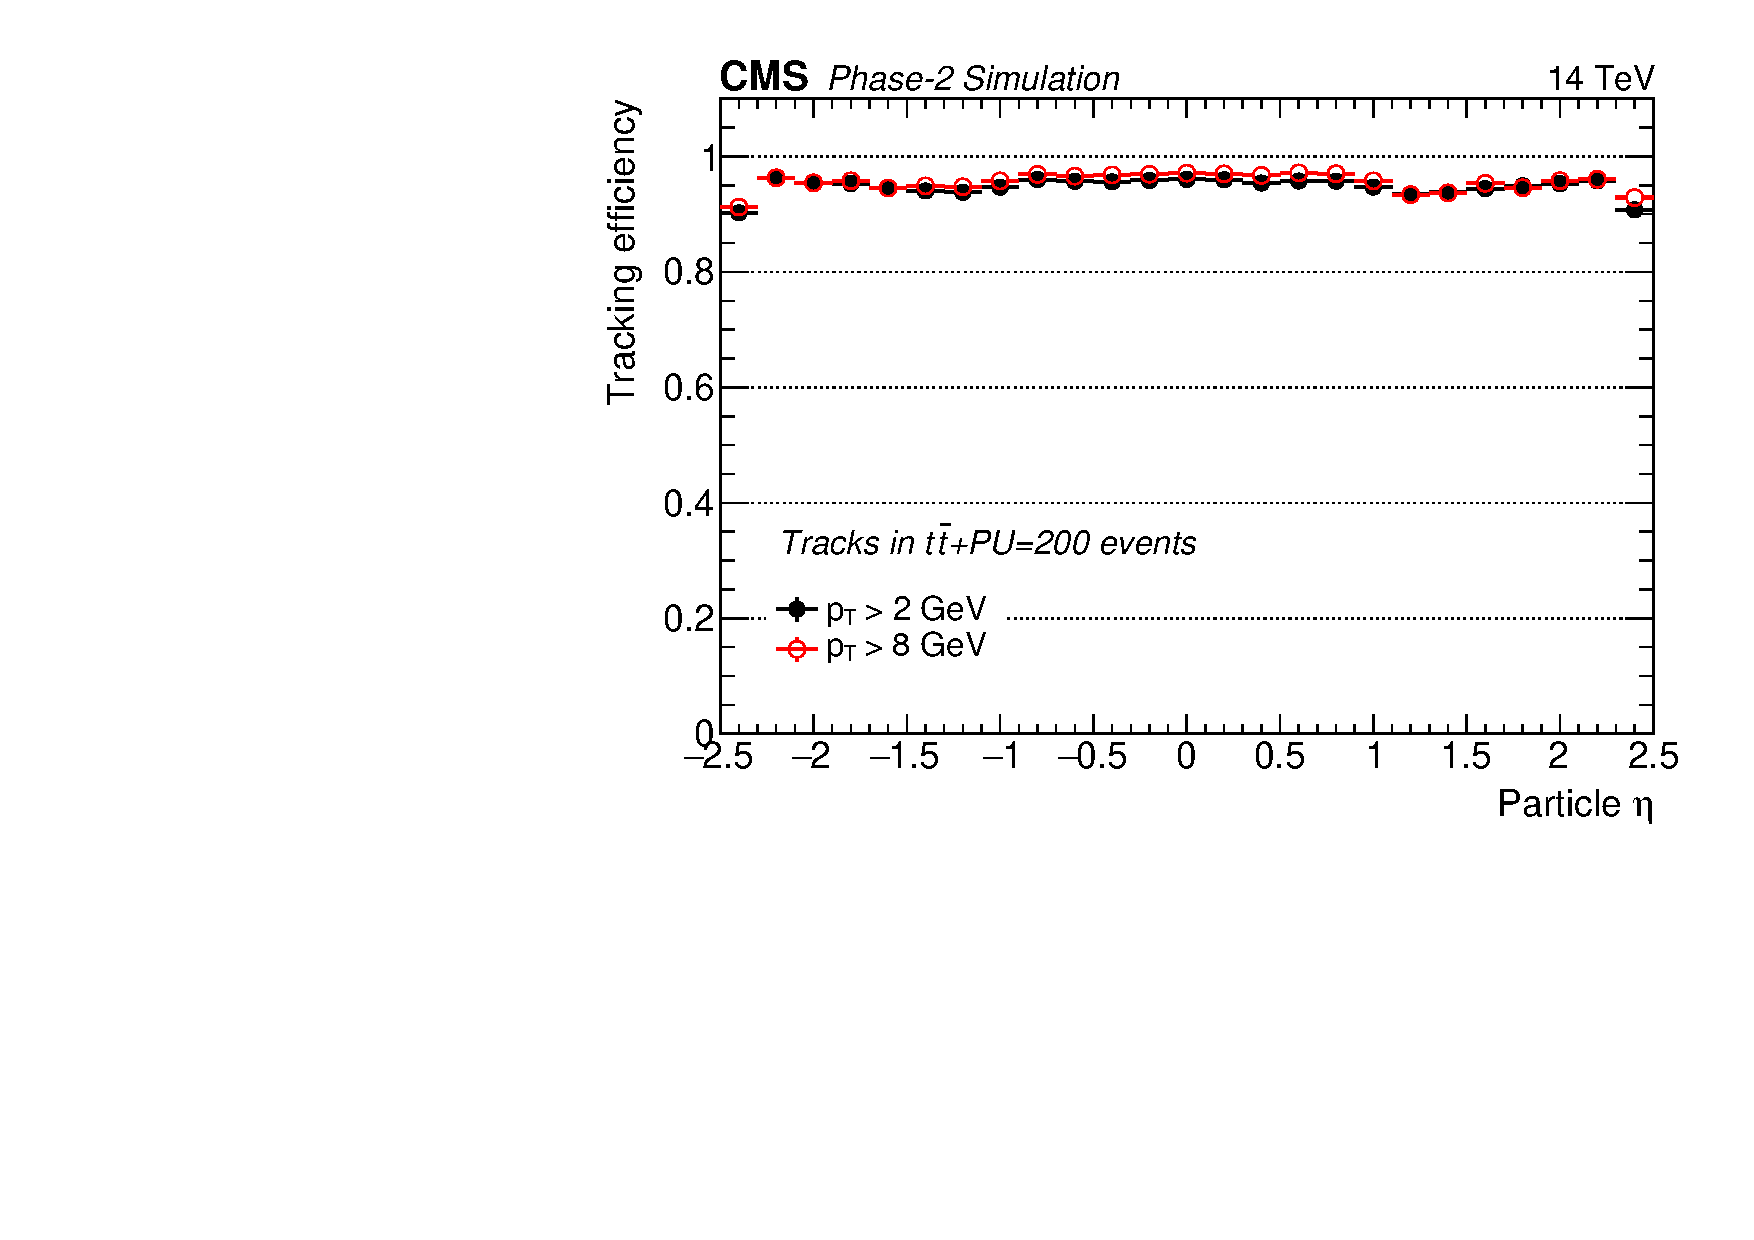
\includegraphics[width=.45\linewidth]{figures/Part2/Upgrade/L1TK_ttbar-pu200_eff_eta}&
  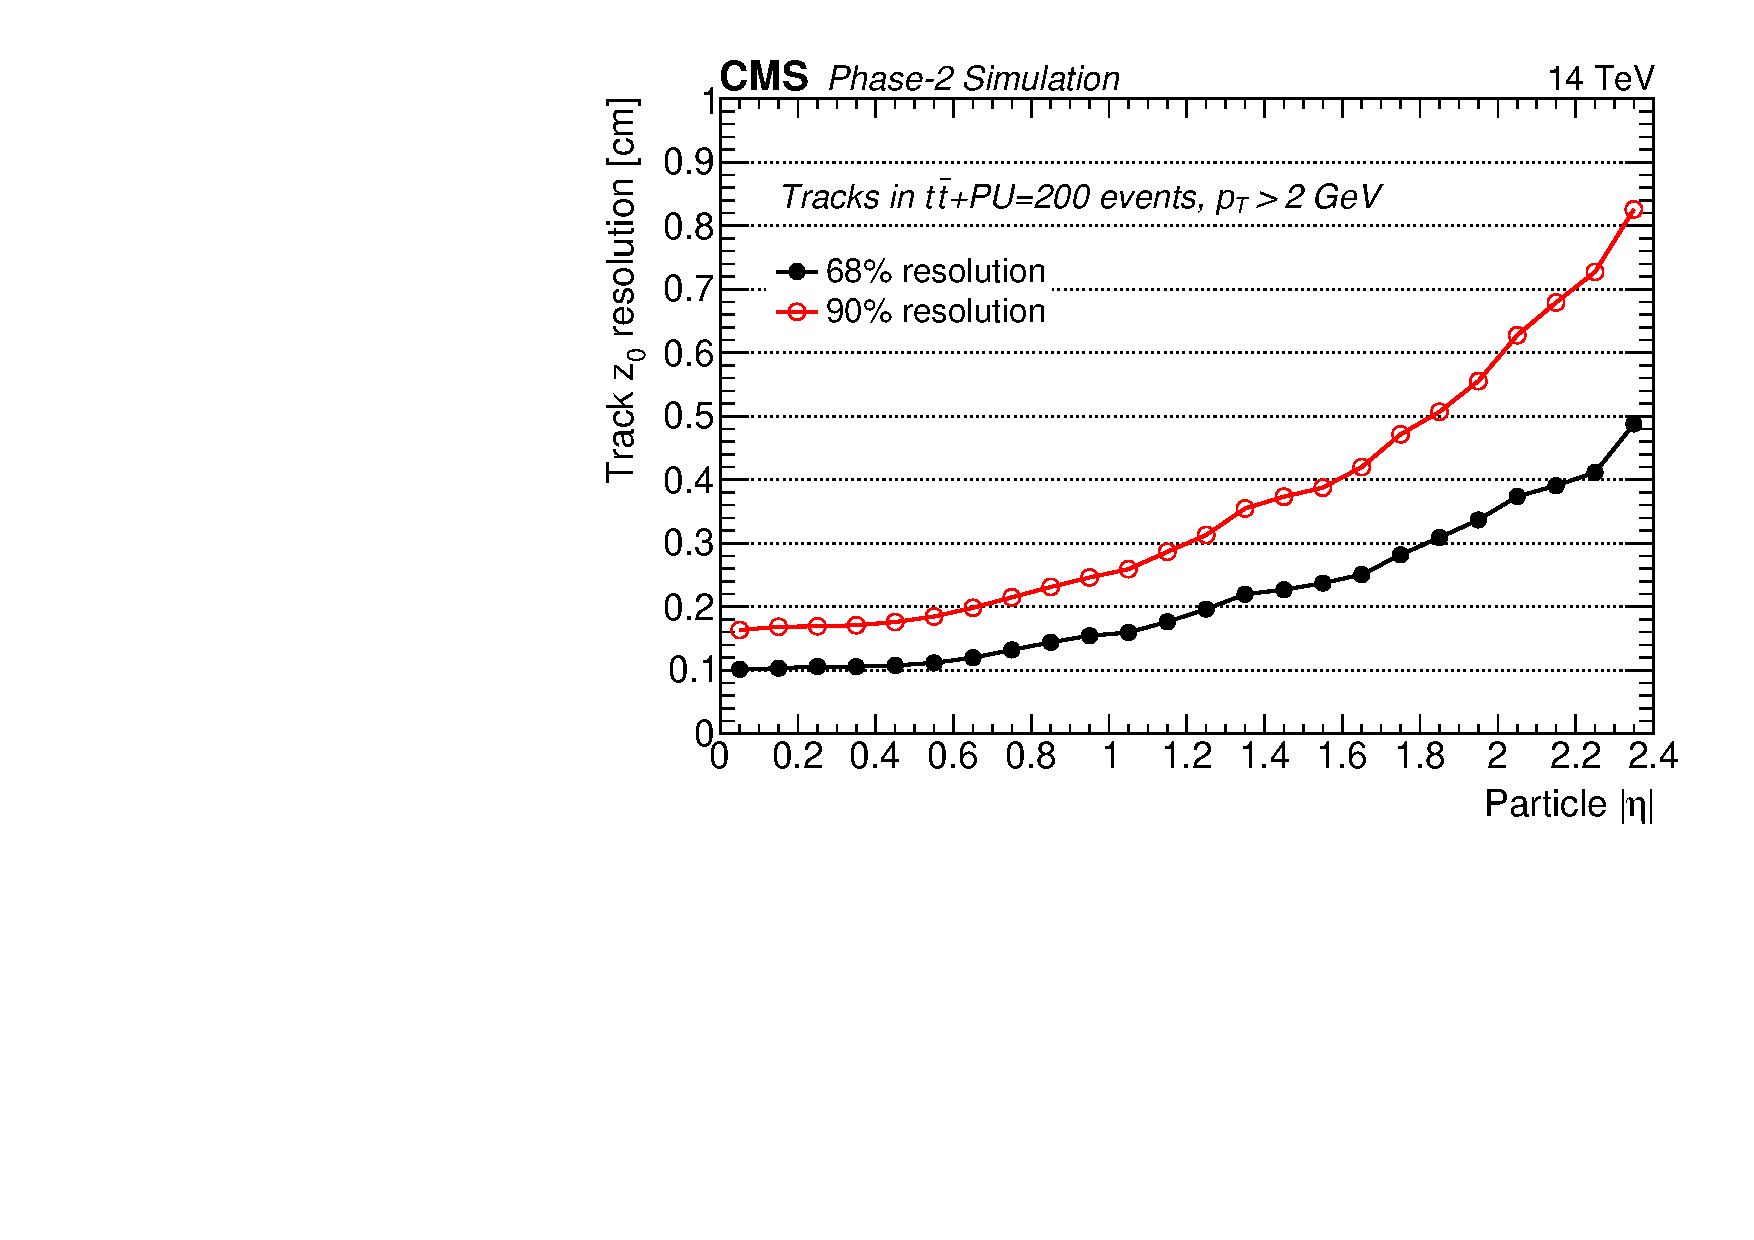
\includegraphics[width=.45\linewidth]{figures/Part2/Upgrade/L1TK_ttbar-pu200_resVsEta_z0}
 \end{tabular}
 \caption{(Tracking efficiency vs particle $\eta$, measured in $\ttbar$ samples (left). Track $z_0$ resolution vs particle $\eta$ (right).}
 \label{fig:trackingperformance}
 \end{center}
\end{figure} 

 \begin{figure}[tbh!]
 \begin{center}
 \begin{tabular}{cc}
  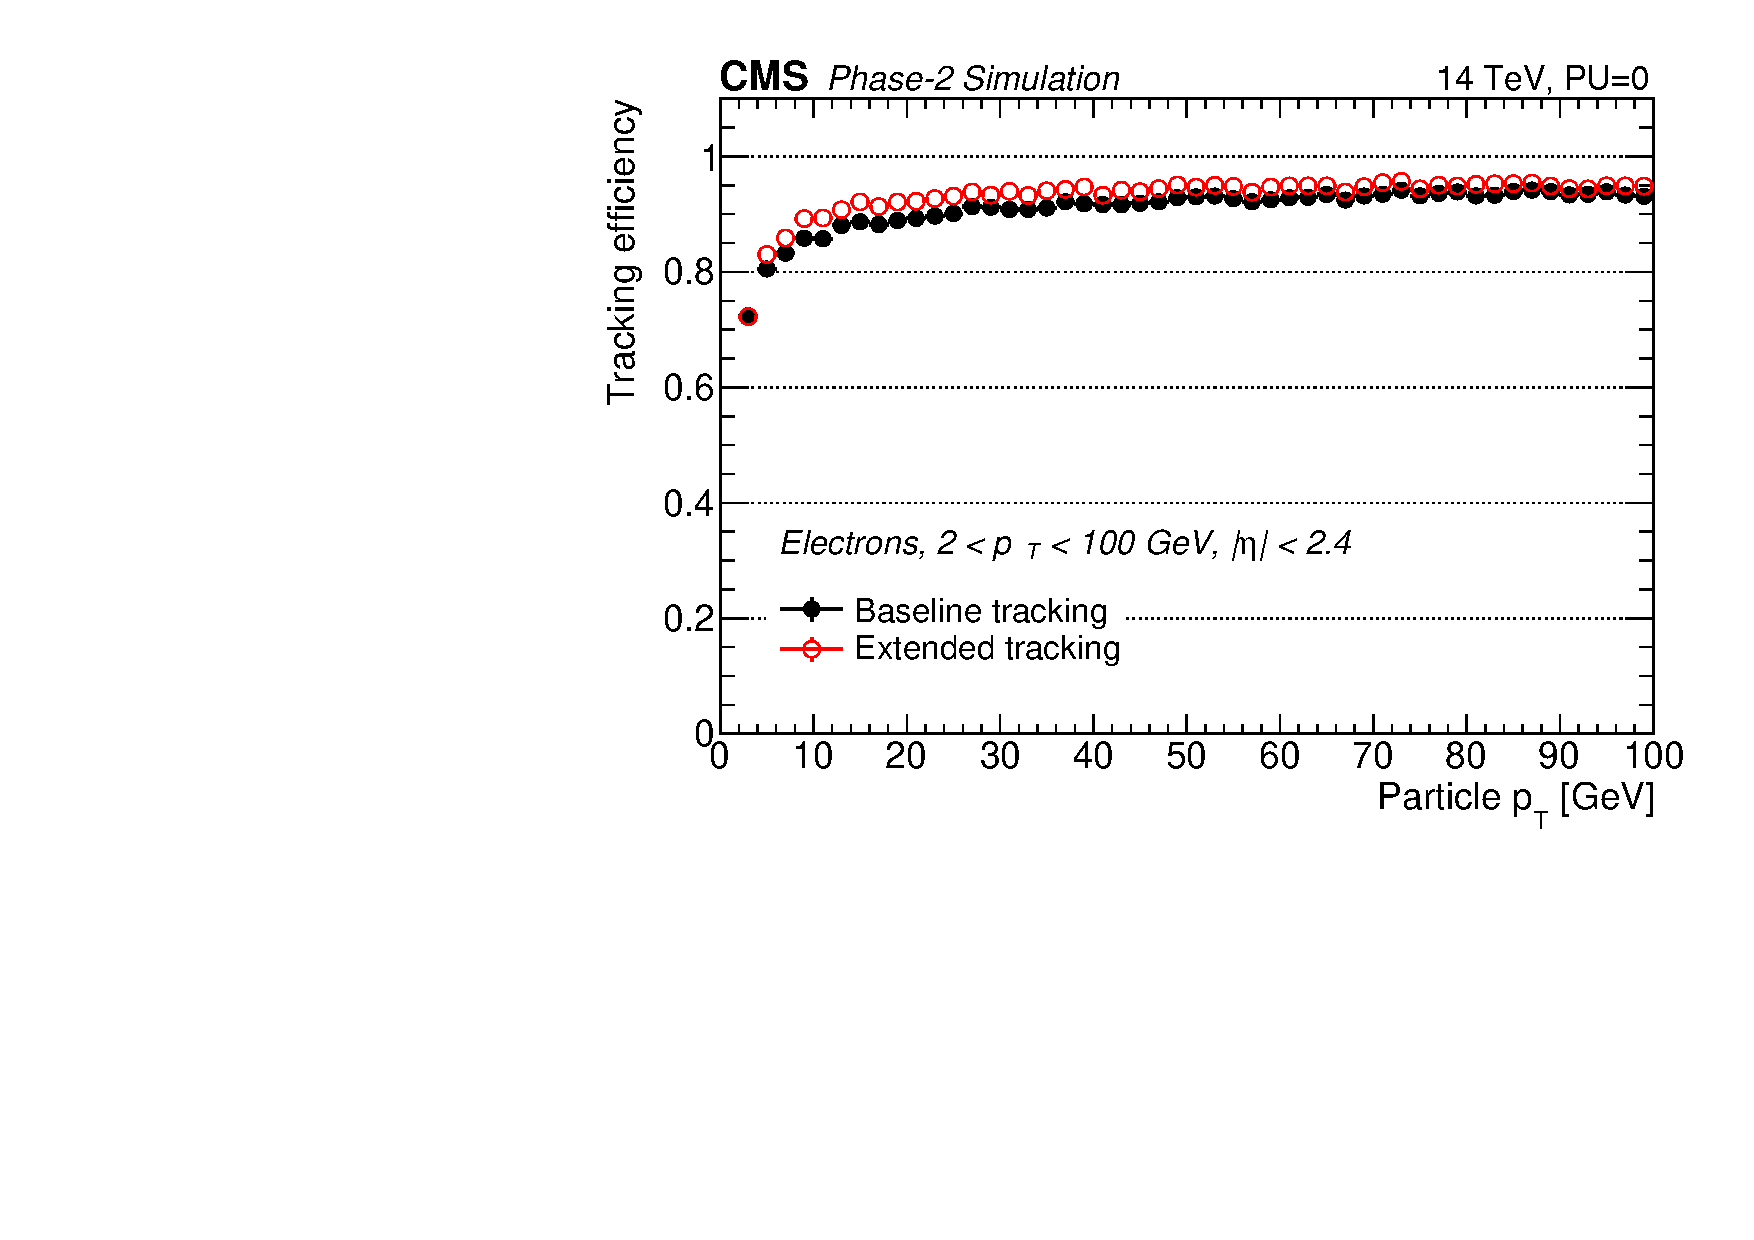
\includegraphics[width=.45\linewidth]{figures/Part2/Upgrade/L1TK_elec-pu0_eff_pt}&
  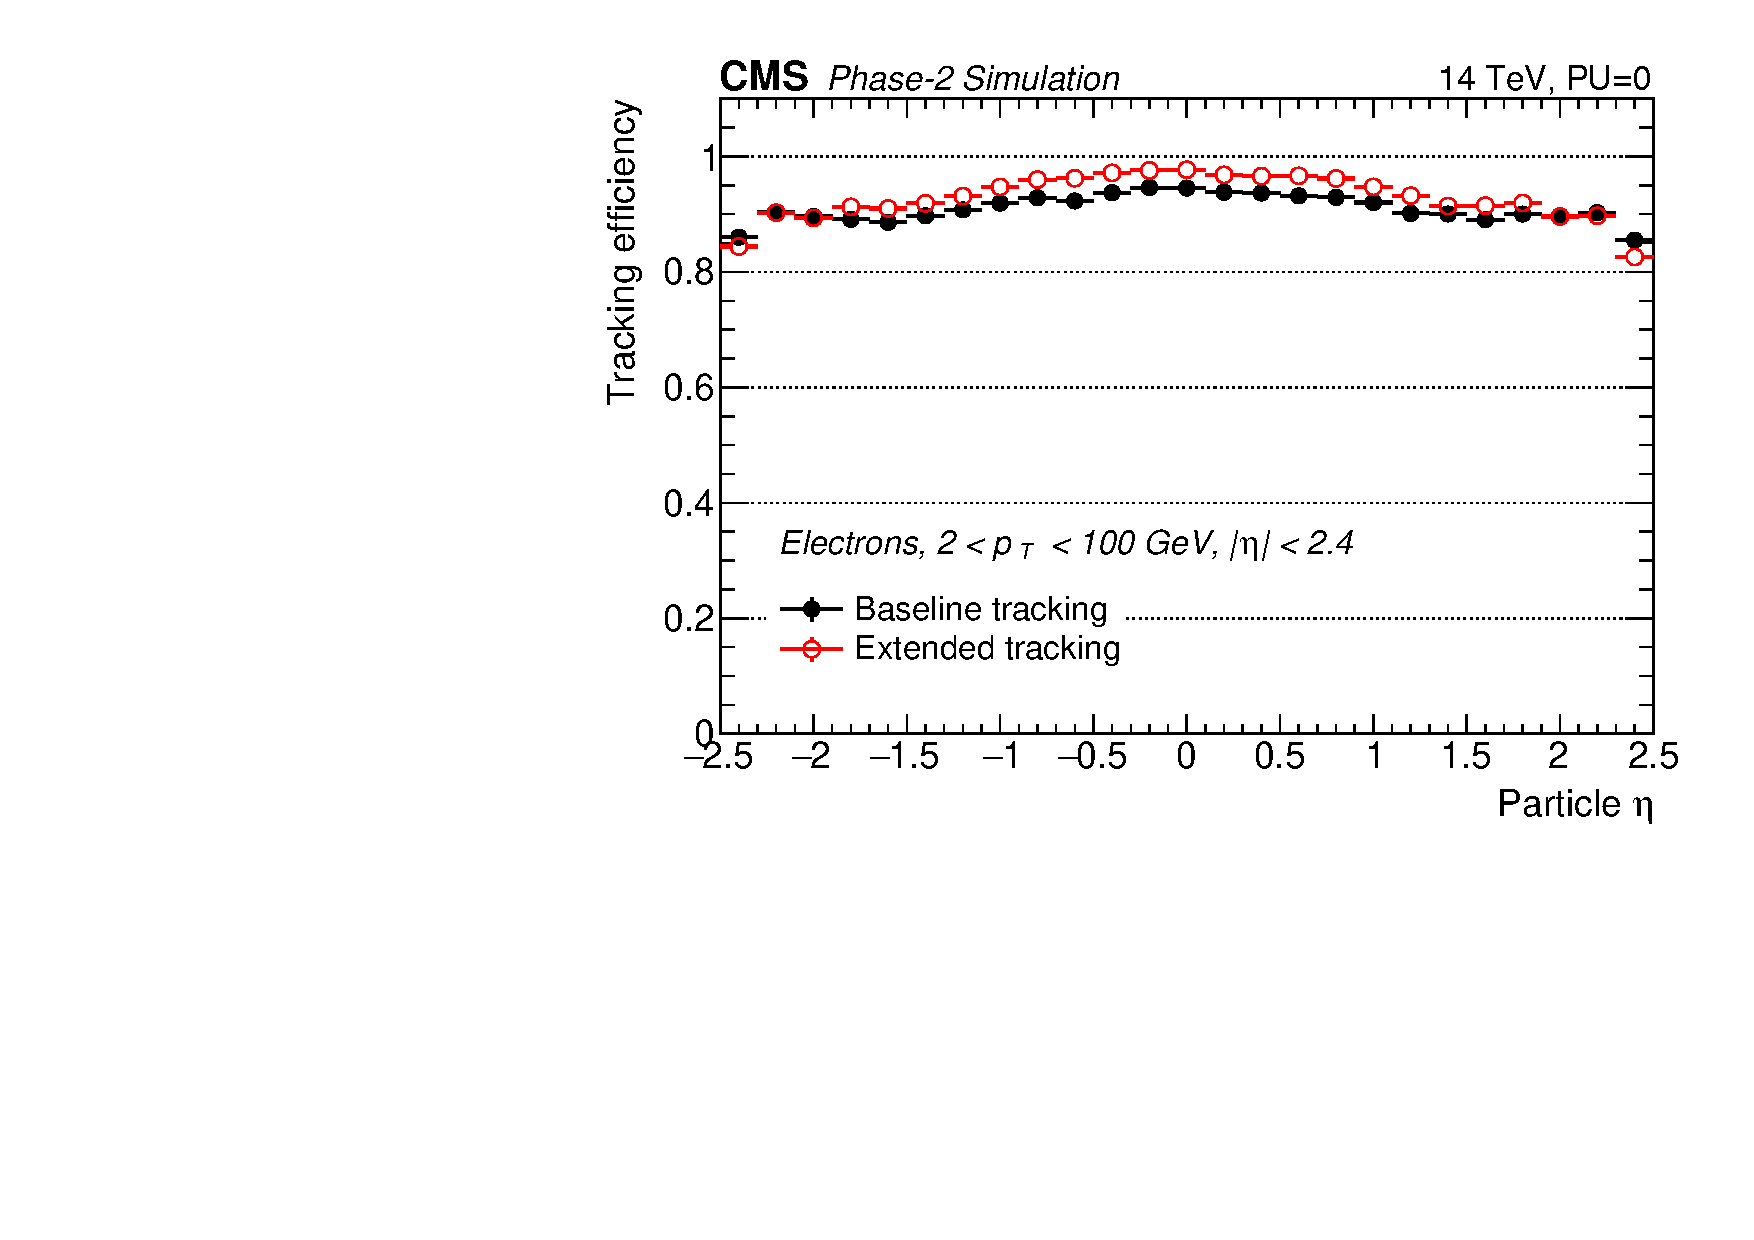
\includegraphics[width=.45\linewidth]{figures/Part2/Upgrade/L1TK_elec-pu0_eff_eta}
 \end{tabular}
 \caption{(Electron tracking efficiency vs particle $\pt$ (left) and $\eta$ (right), measured in simulated electron samples with 0 \ac{PU}.}
 \label{fig:electronperformance}
 \end{center}
\end{figure} 

\section{Leve-1 Electron Trigger Algorithm}
\label{sec:L1Ele}

With the increase of the instantaneous luminosity, triggering on electrons at \ac{L1} will face unprecedented challenges as the data volume generated in the calorimeters becomes too large for the legacy trigger algorithms. The addition of tracking information provides a much-needed handle for the electron trigger. It enables precise track-calorimeter shower matching to control the trigger rate. To take advantage of this new tool, a new electron trigger algorithm is developed and documented in Ref.~\cite{Zabi:2020gjd}. 

The central feature of this algorithm is the fine-tuned matching between tracks produced by the \ac{L1} track finder and calorimeter clusters reconstructed in the \ac{ECAL} Barrel or \ac{HGCAL}. The baseline version of this algorithm extrapolates tracks to the calorimeter surface using the track $\pt$ and matches them with calorimeter clusters. An elliptical cut in the $\eta-\phi$ plane is applied and illustrated in Figure~\ref{fig:electron}.
  
 \begin{figure}[tbh!]
 \begin{center}
 \begin{tabular}{ccc}
  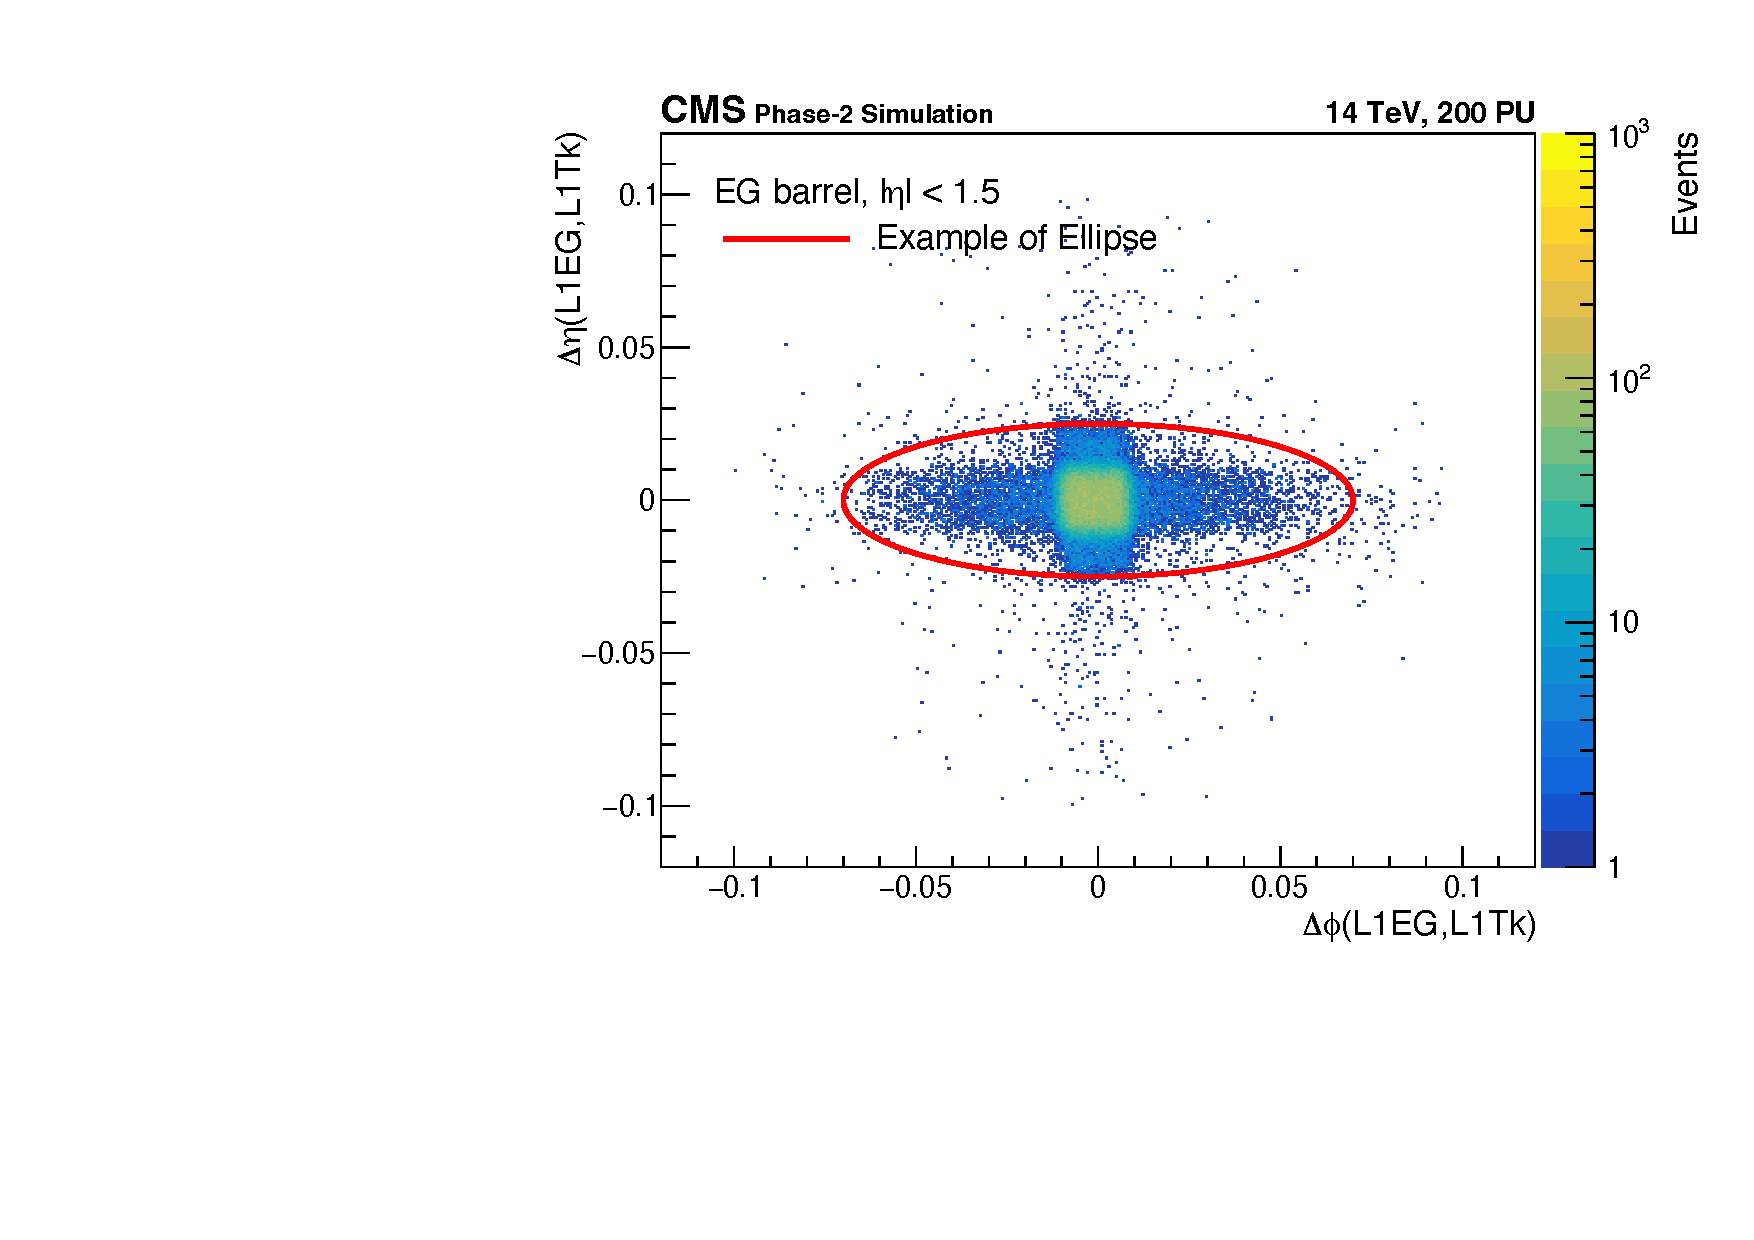
\includegraphics[width=.45\linewidth]{figures/Part2/Upgrade/DR_barrel}&
  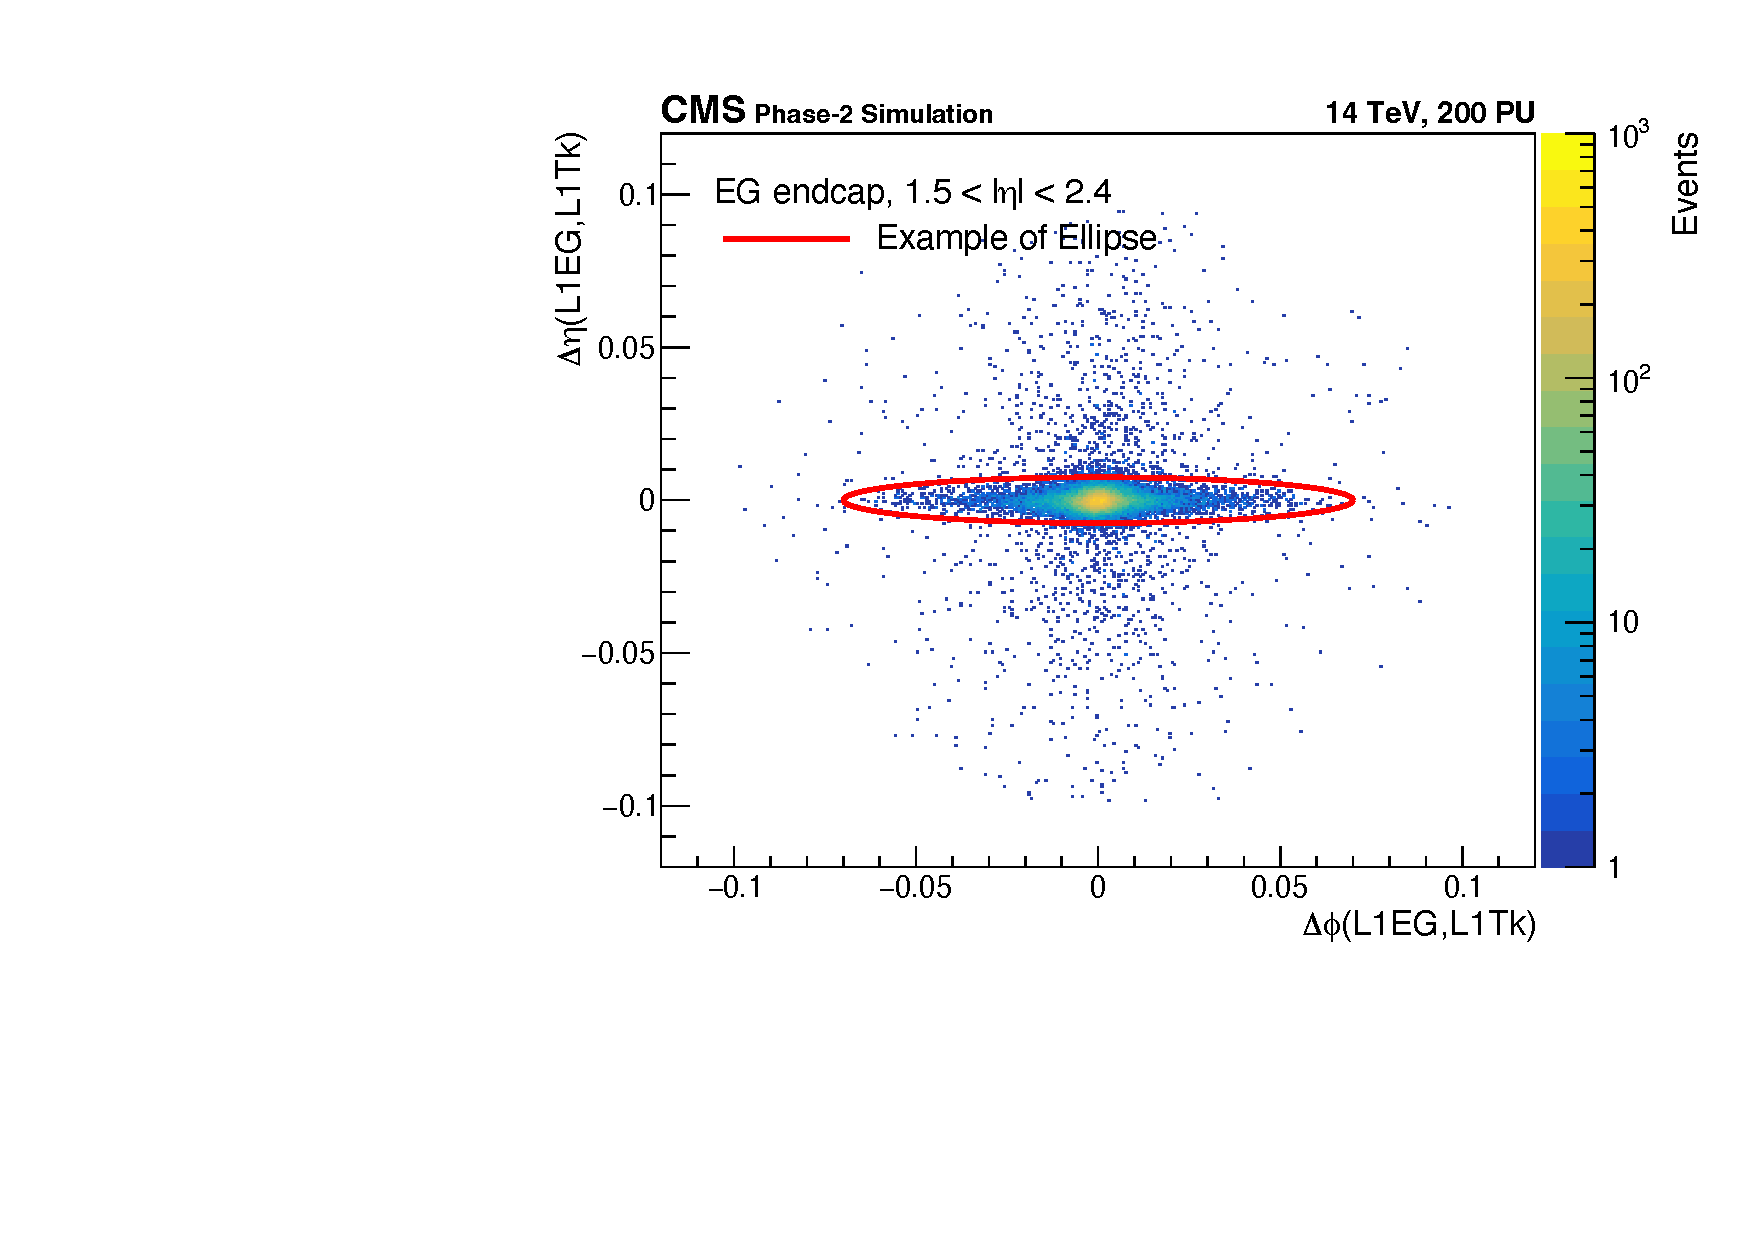
\includegraphics[width=.45\linewidth]{figures/Part2/Upgrade/DR_endcap}&
 \end{tabular}
 \caption{$\mathrm{\Delta}\eta$ vs $\mathrm{\Delta}\phi$ distances between calorimeter clusters and the closest \ac{L1} track in the \ac{ECAL} Barrel (left) and \ac{HGCAL}. Tracks are extrapolated using track $\pt$.}
 \label{fig:electron}
 \end{center}
\end{figure}

The baseline algorithm provides roughly a factor of three reduction in event rate while keeping the efficiency loss under control, as shown in Table~\ref{tab:L1EleRate}-Table~\ref{tab:L1EleEff}. The efficiency loss is largely driven by the inefficiencies in electron tracking, as illustrated in Figure~\ref{fig:electronperformance}.

\begin{table}[th]
\sffamily
\centering
\caption{Trigger rate of \ac{L1} trigger objects in the \ac{ECAL} Barrel. Data in the first column shows the two reference trigger thresholds.}
\begin{tabular}{ccc} \toprule
Rate & calorimeter only & track-matched \\  \midrule
 30 GeV   & 78.2 kHz   & 19.0 kHz\\ \midrule
 40 GeV & 25.5 kHz   & 8.3 kHz\\ \bottomrule
\end{tabular}
\label{tab:L1EleRate}
\end{table}

\begin{table}[th]
\sffamily
\centering
\caption{Trigger efficiency for \ac{L1} trigger objects computed at two reference trigger thresholds in the \ac{ECAL} Barrel. }
\begin{tabular}{ccc} \toprule
Efficiency & calorimeter only & track-matched \\  \midrule
 30 GeV   & 97.5\%   & 84.5\%\\ \midrule
 40 GeV & 98.7\%   & 88.0\%\\ \bottomrule
\end{tabular}
\label{tab:L1EleEff}
\end{table}

An alternative version of this algorithm uses the energy estimate from the calorimeter instead of the Outer Tracker to extrapolate \ac{L1} tracks. The superior energy resolution delivered by the calorimeters further constrains the projected track $\eta$ and $\phi$ coordinates to the targeted calorimeter clusters, as illustrated in \ref{fig:DR_electron}. This enables the implementation of a much tighter ellipse in the $\eta-\phi$ plane.

\begin{figure}[tbh!]
 \begin{center}
 \begin{tabular}{ccc}
  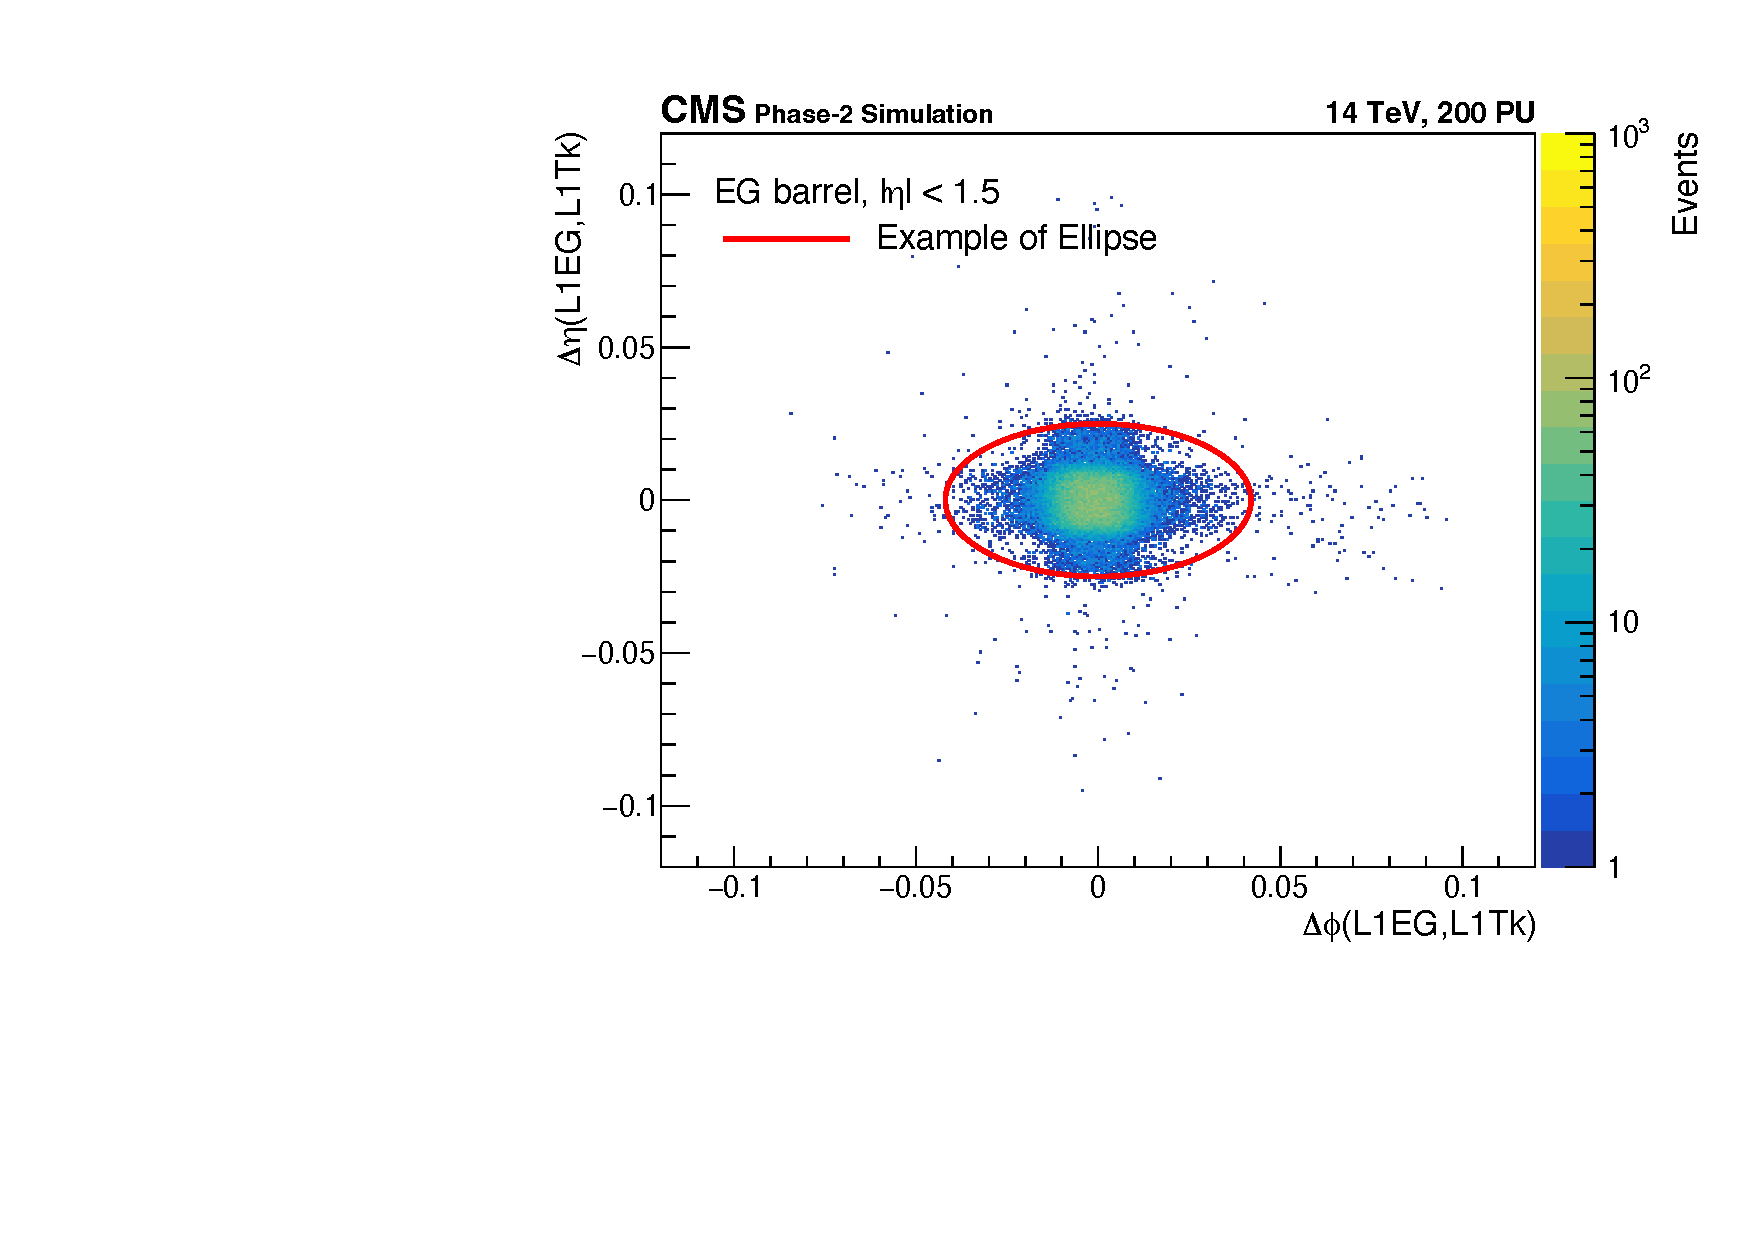
\includegraphics[width=.45\linewidth]{figures/Part2/Upgrade/DR_barrel_new}&
  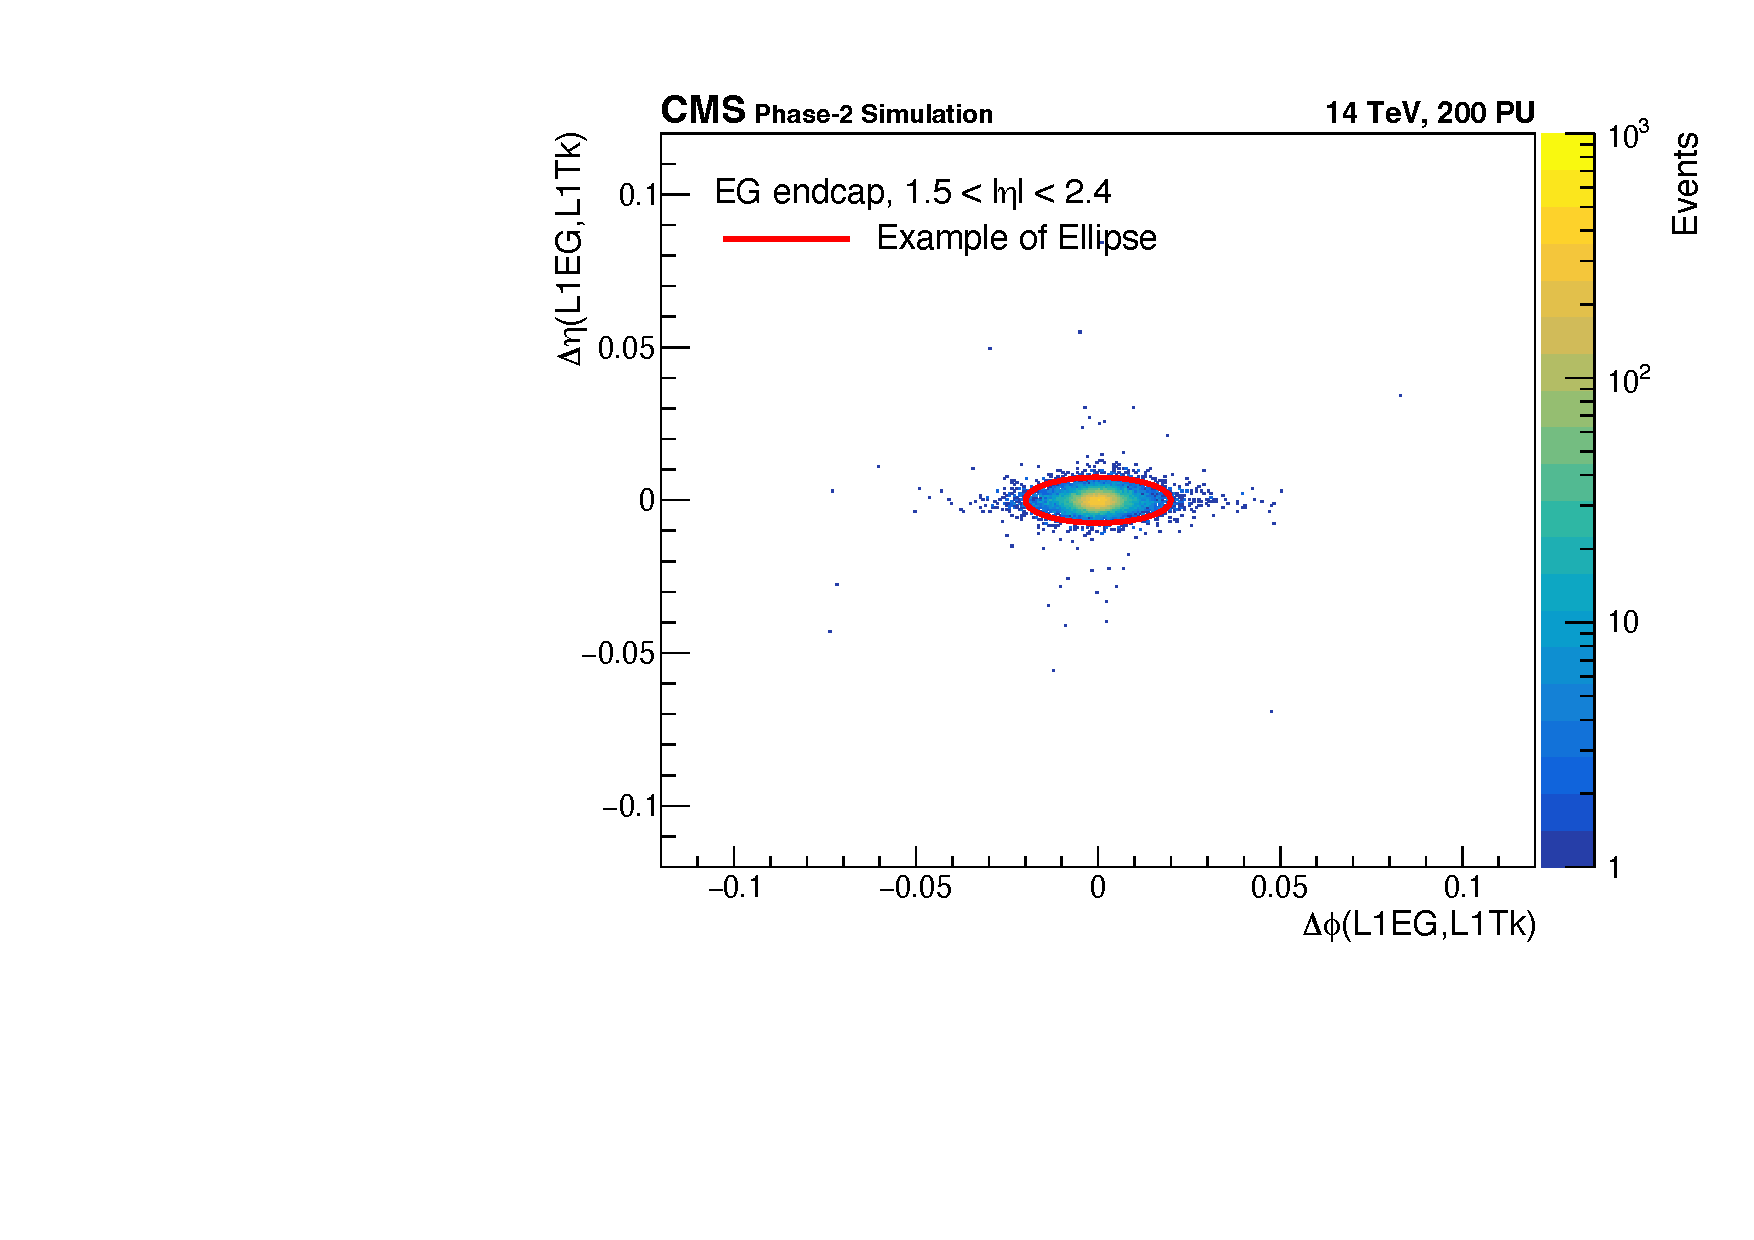
\includegraphics[width=.45\linewidth]{figures/Part2/Upgrade/DR_endcap_new}&
 \end{tabular}
 \caption{$\mathrm{\Delta}\eta$ vs $\mathrm{\Delta}\phi$ distances between calorimeter clusters and the closest L1 track in the \ac{ECAL} Barrel (left) and \ac{HGCAL}. Tracks are extrapolated using energy estimates from the calorimeter.}
 \label{fig:DR_electron}
 \end{center}
\end{figure}

A comparison between two versions of the electron trigger algorithms is shown in Figure~\ref{fig:rate_electron}-\ref{fig:eff_electron}. 

 \begin{figure}[tbh!]
 \begin{center}
 \begin{tabular}{ccc}
  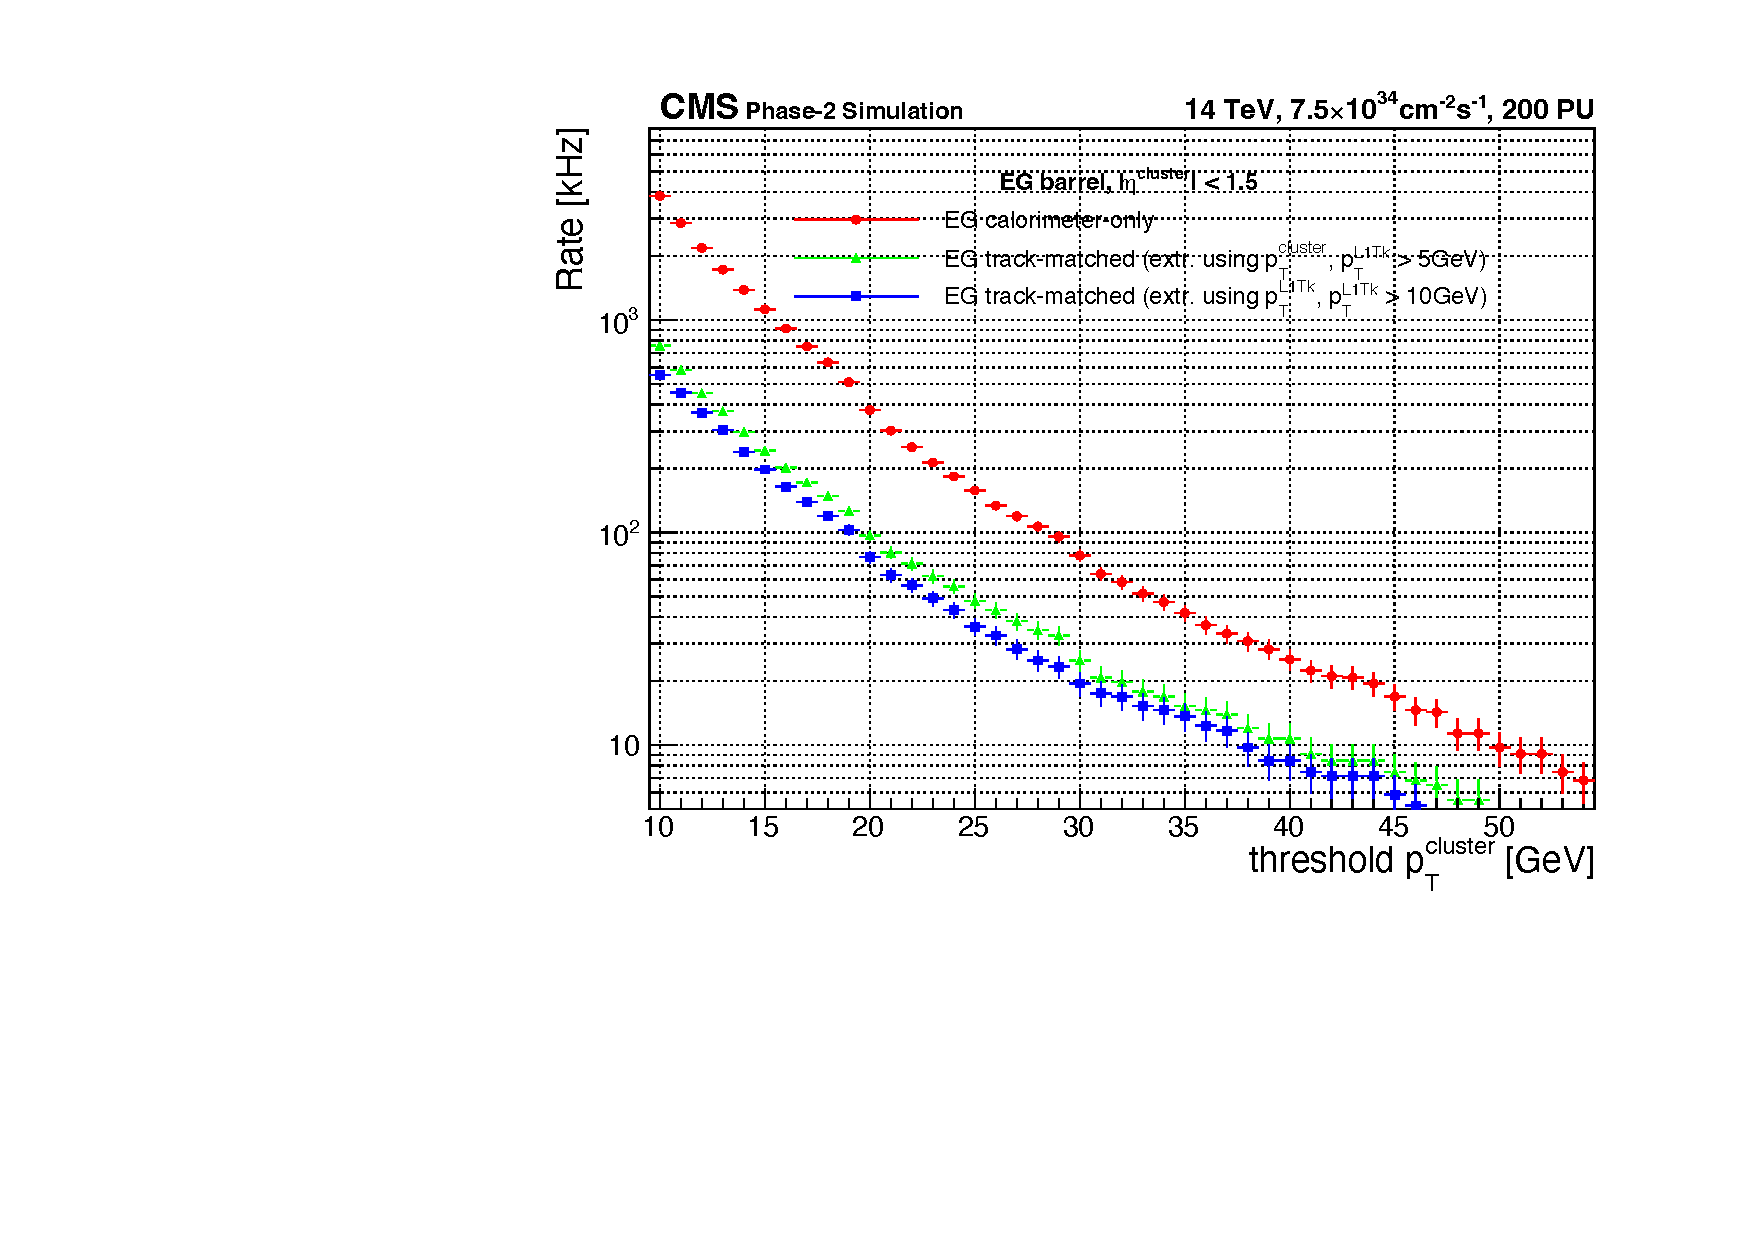
\includegraphics[width=.45\linewidth]{figures/Part2/Upgrade/Rate_barrel}&
  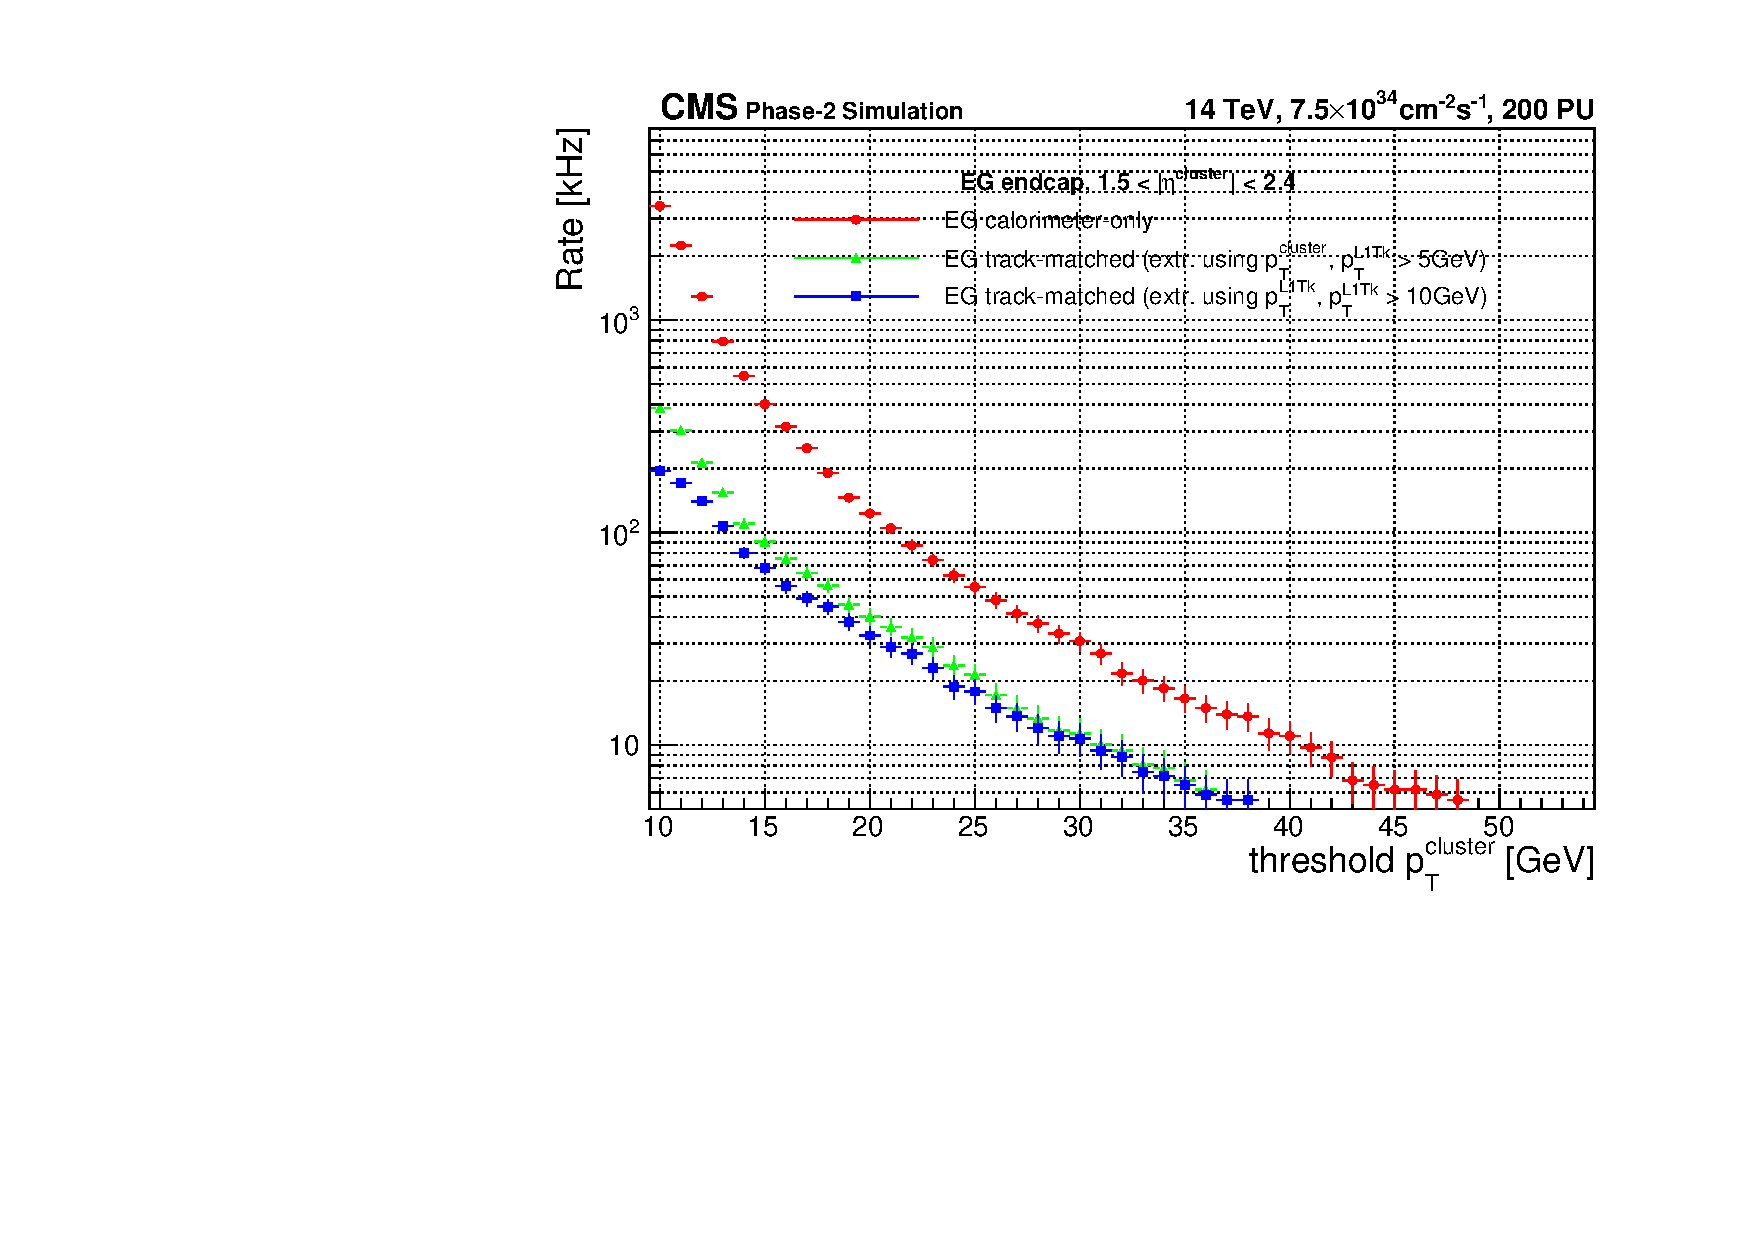
\includegraphics[width=.45\linewidth]{figures/Part2/Upgrade/Rate_endcap}&
 \end{tabular}
 \caption{\ac{L1} event rate as a function of the electron trigger threshold in the \ac{ECAL} Barrel (left) and \ac{HGCAL} (right). The event rate computed for calorimeter-only objects is shown in red data points. Event rates computed for the objects reconstructed by the baseline and alternative electron trigger algorithms are represented with blue and green data points, respectively.}
 \label{fig:rate_electron}
 \end{center}
\end{figure}

 \begin{figure}[tbh!]
 \begin{center}
 \begin{tabular}{ccc}
  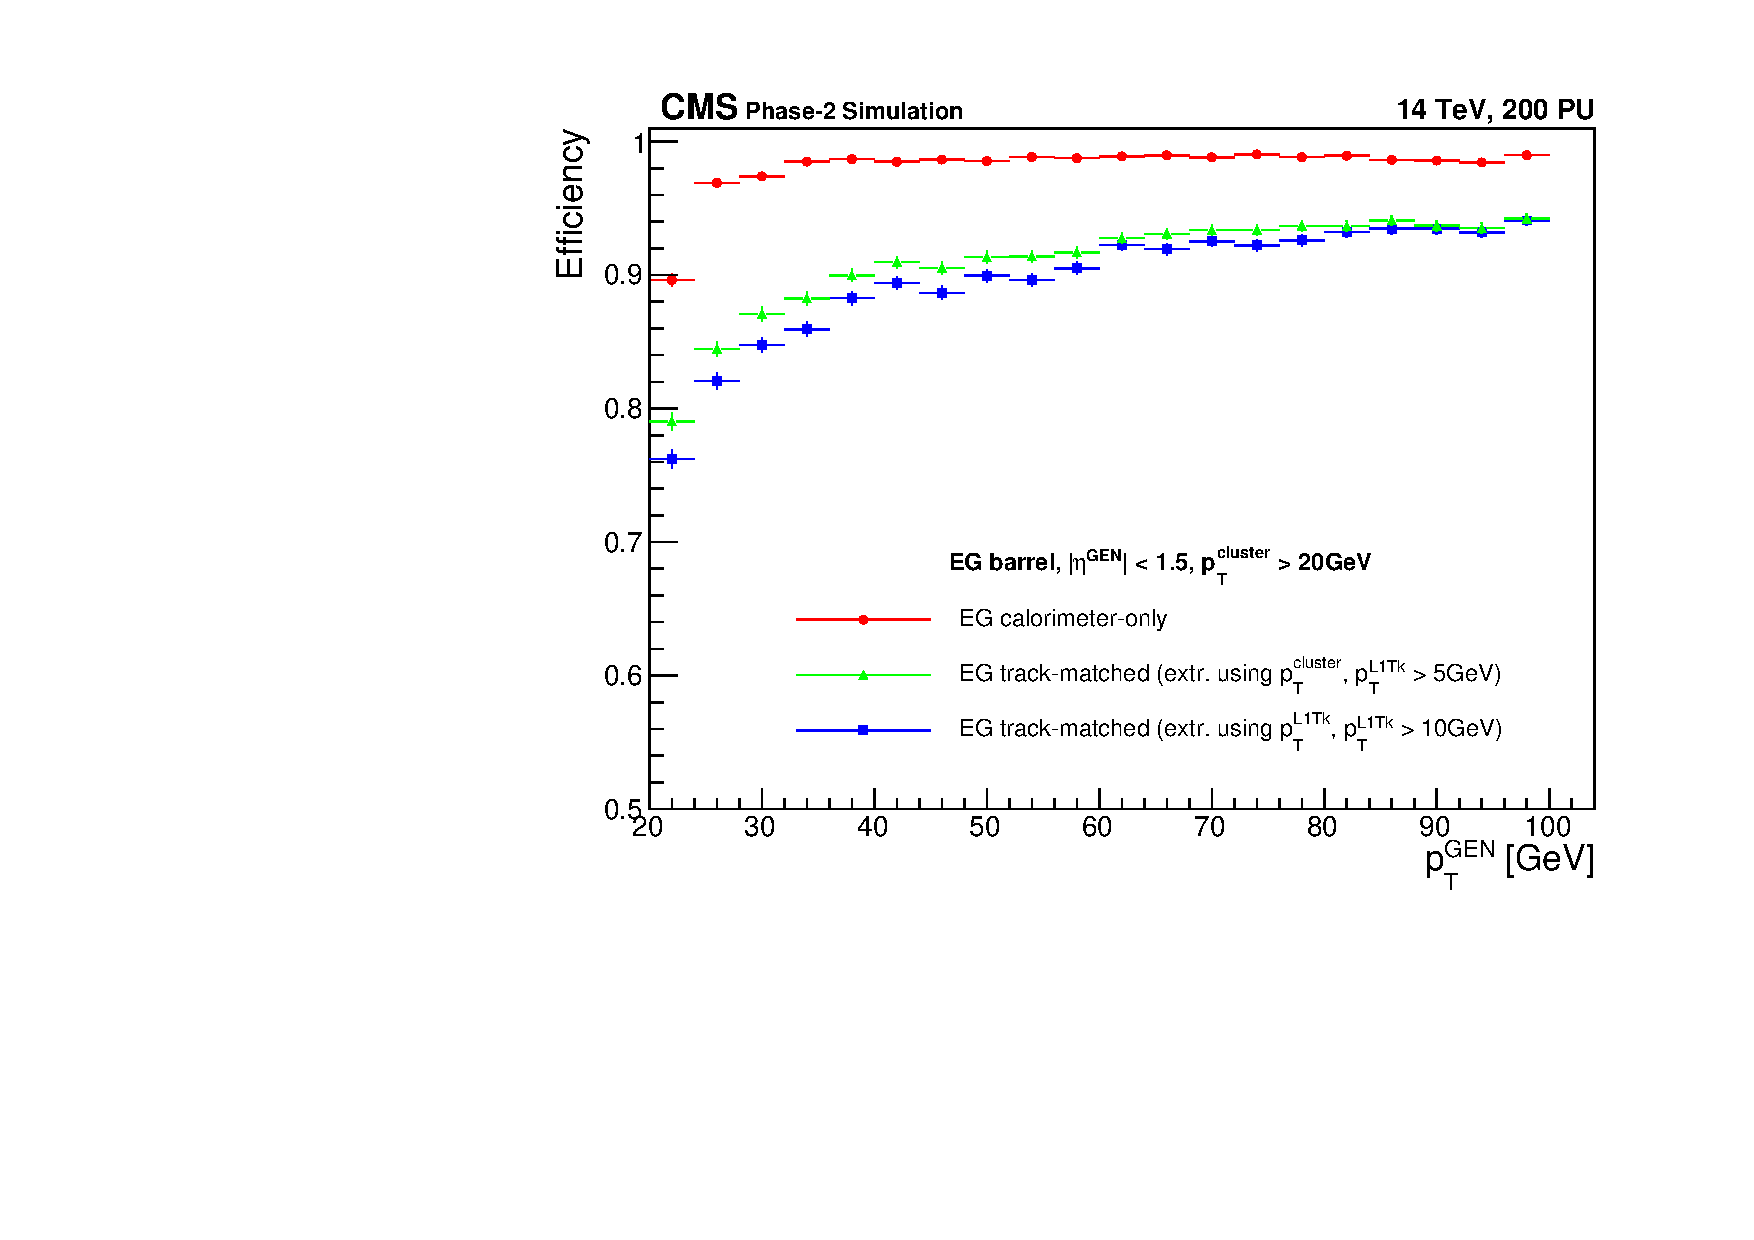
\includegraphics[width=.45\linewidth]{figures/Part2/Upgrade/eff_barrel}&
  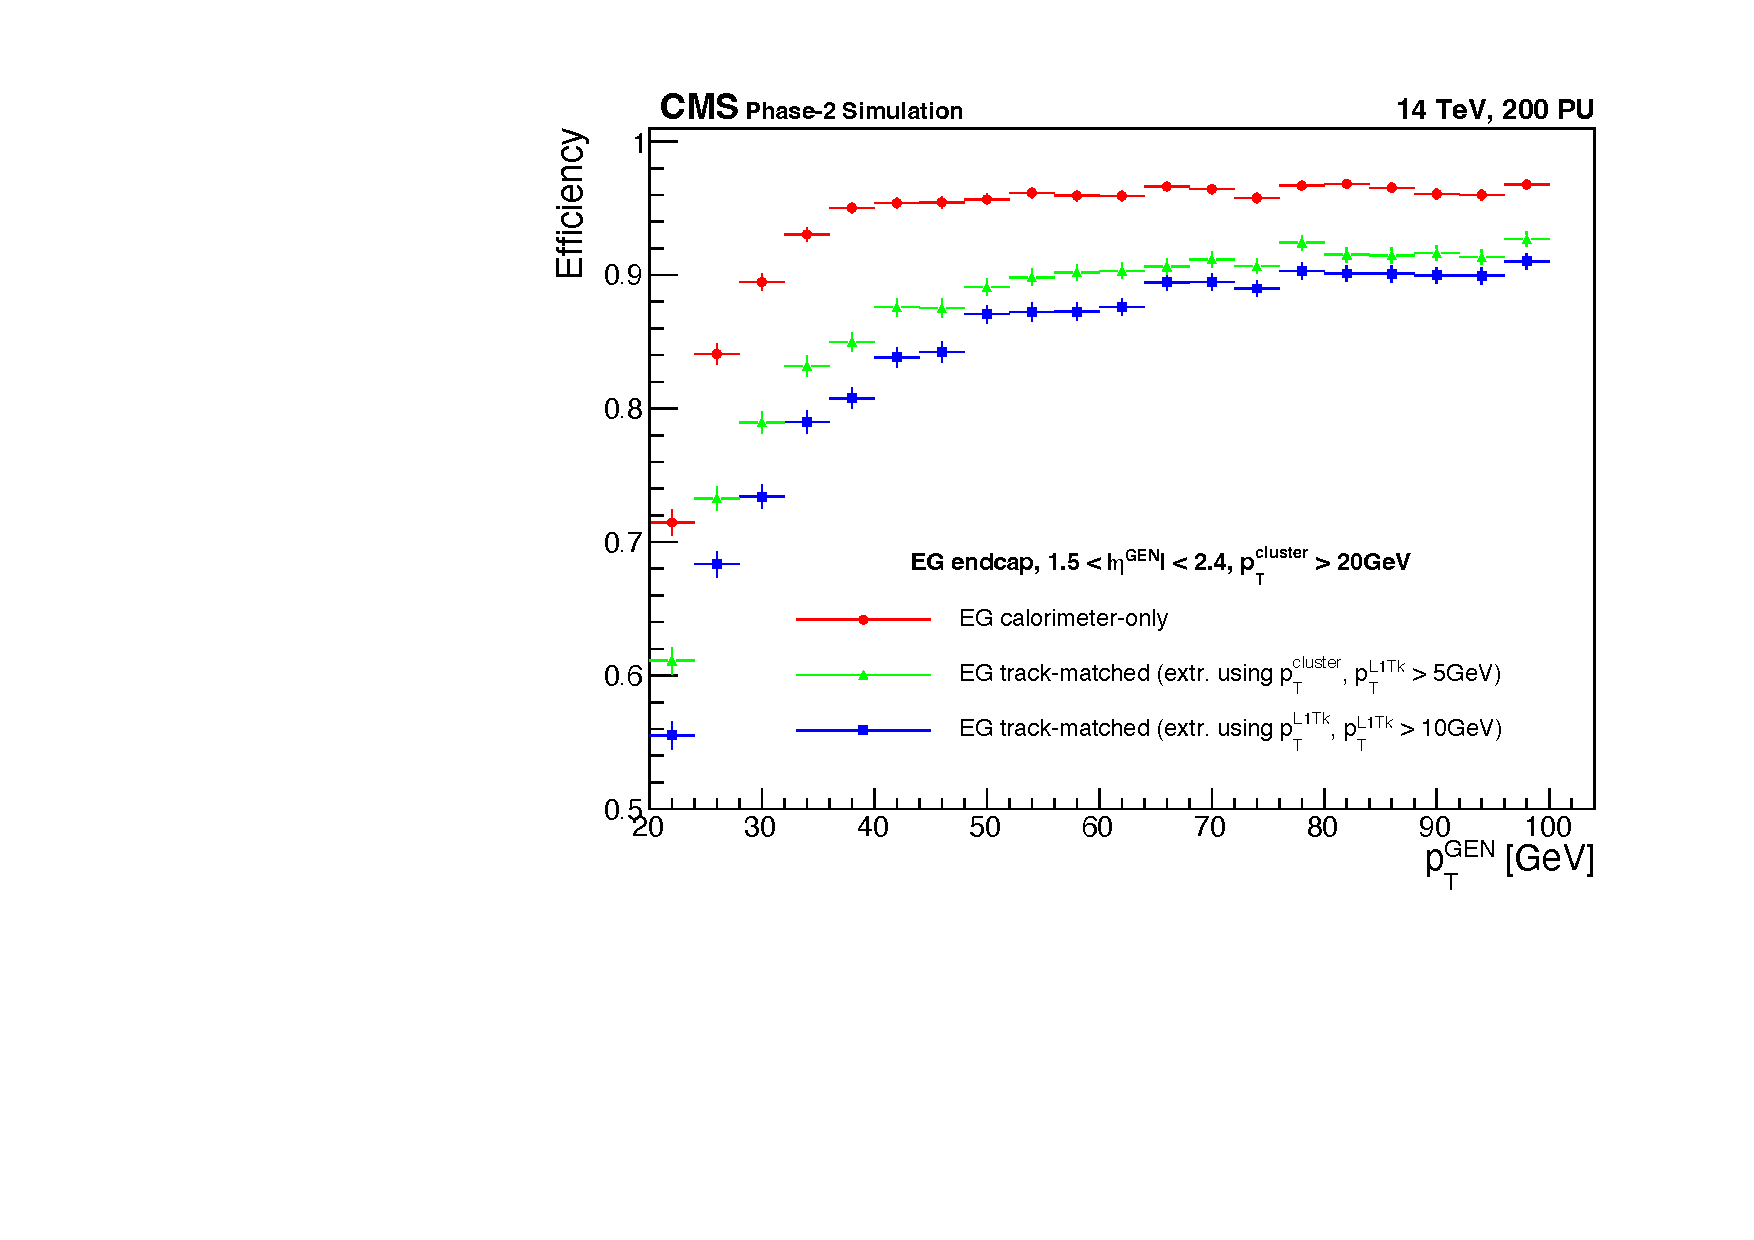
\includegraphics[width=.45\linewidth]{figures/Part2/Upgrade/eff_endcap}&
 \end{tabular}
 \caption{\ac{L1} electron trigger efficiency as a function of the particle $\pt$ in the \ac{ECAL} Barrel (left) and \ac{HGCAL} (right). The efficiency computed for calorimeter-only objects is shown in red data points. Efficiencies computed for the objects reconstructed by the baseline and alternative electron trigger algorithms are represented with blue and green data points, respectively.}
 \label{fig:eff_electron}
 \end{center}
\end{figure}

When compared to the older electron trigger algorithms~\cite{CMS:2017lum}, this newly designed algorithm (baseline) improves the electron reconstruction efficiency at \ac{L1} by 5\% while reducing the background rate by a factor of 2.  
